\section{Introduction}
\subsection{Contexte}

L’objectif du projet est de classifier automatiquement des cellules sanguines à partir d’images de frottis sanguins.

D’un point de vue technique, le projet couvre l’ensemble de la chaîne de traitement : exploration et visualisation d’images de frottis sanguins issues de deux sources hétérogènes, prétraitement et harmonisation (normalisation colorimétrique, augmentation) pour constituer un jeu de données fusionné exploitable, puis conception et entraînement de modèles de réseaux de neurones convolutifs à l'aide d'un framework permettant de reproduire les différentes configurations.

Sur le plan économique, l’automatisation de certaines étapes d’analyse peut contribuer à réduire le temps consacré aux tâches répétitives et à améliorer l’efficacité du processus d’analyse.

Plusieurs difficultés sont apparues dès l’analyse des données. Les classes sont fortement déséquilibrées, avec jusqu’à 17 fois plus d’exemples pour la classe majoritaire que pour la plus rare. Le coût des erreurs n’est pas non plus symétrique : manquer une cellule critique est plus problématique qu’une fausse alerte. Enfin, les deux sources présentent un biais de domaine qui reste visible malgré les étapes d’harmonisation.
Ces trois points ont directement influencé les choix de prétraitement, de fonction de perte et de métriques.

\subsection{Objectifs}

L’objectif principal de ce projet est de préparer et exploiter un jeu de données d’images de cellules sanguines afin de permettre leur classification automatique, aussi bien au niveau du type cellulaire fin qu’au niveau clinique (normal / anormal, criticité).
Il s’agit dans un premier temps d’explorer les données pour en évaluer la qualité, la répartition et les caractéristiques, puis de réaliser les étapes de visualisation et de pré-processing nécessaires à leur utilisation.
Le preprocessing vise ainsi à obtenir un jeu de données fiable, homogène et adapté à l’entraînement et à l’évaluation des modèles de classification.
Au-delà de l’entraînement de ces modèles, le projet vise également à \textbf{comparer les performances obtenues aux modèles existants} dans la littérature, et à \textbf{proposer une fonction de perte ainsi que des métriques d’évaluation adaptées} au déséquilibre des classes et à l’asymétrie clinique du coût des erreurs, plutôt que de s’appuyer sur des critères génériques comme l’accuracy.

Les membres du groupe présentent des niveaux d’expertise complémentaires autour de la problématique de classification des cellules sanguines.

\textbf{Rémi} et \textbf{Romain} ont adopté une approche centrée sur l’exploration et la compréhension des données.
Leur travail porte notamment sur l’analyse des métadonnées, la visualisation des distributions, l’identification des différences entre les sources de données ainsi que sur les premières étapes de nettoyage et de pré-processing.
Ce travail nous a permis de mieux comprendre la structure du jeu de données avant de passer aux modèles.

\textbf{Joseph} a davantage abordé la problématique par la modélisation.
Il a entraîné des modèles de classification binaire, avec un modèle dédié à chaque type de cellule, afin d’évaluer directement la capacité des données à permettre la discrimination entre les classes.
Cette approche lui a également permis d'identifier les éventuels problèmes de qualité ou de nettoyage des données à partir des résultats obtenus.

Cette répartition se prolonge, avec des rôles affinés, lors de la phase de modélisation proprement dite.
\textbf{Romain} s’est concentré sur le framework d’entraînement garantissant la reproductibilité des expériences (configuration versionnée, recherche par grille, suivi systématique des résultats), ainsi que sur la conception de la fonction de perte et des métriques adaptées au déséquilibre des classes et à l’asymétrie clinique du coût des erreurs ; ce travail a été validé sur un modèle \emph{baseline}.
\textbf{Rémi} a exploré des architectures de réseaux de neurones plus avancées ainsi que des approches par transfert d’apprentissage (\emph{transfer learning}).
\textbf{Joseph} a poursuivi son travail de modélisation binaire par cellule et a développé un modèle hiérarchique.

Les différentes approches sont donc complémentaires : l’exploration et le pré-processing permettent de comprendre et de fiabiliser les données, tandis que la modélisation (framework d’expérimentation, fonction de perte et métriques, architectures avancées et transfert, approches binaire et hiérarchique) permet de confronter ces choix à leur impact sur les performances de classification.


\section{Compréhension et manipulation des données}
\subsection{Cadre}

Le projet s’appuie sur deux jeux de données d’images de cellules sanguines, accessibles librement et regroupant des images acquises dans des contextes cliniques distincts.
Le premier, \textbf{PBC Dataset Normal DIB}, est disponible sur Mendeley Data \parencite{acevedo2020mendeley,acevedo2020dib} ; le second, \textbf{PKG-AML-Cytomorphology\_LMU}, est disponible sur The Cancer Imaging Archive \parencite{matek2019tcia,matek2019nmi}.

Le jeu de données PBC contient \textbf{17\,092 images} de cellules individuelles acquises au laboratoire central de l’hôpital de Barcelone, à partir d’individus sans infection, sans maladie hématologique ou oncologique et ne suivant aucun traitement pharmacologique au moment du prélèvement.
Le jeu de données LMU contient \textbf{18\,365 images} de cellules uniques annotées par des experts, prélevées sur des frottis de sang périphérique de 100 patients diagnostiqués avec une leucémie myéloïde aiguë (LMA) à l’hôpital universitaire de Munich entre 2014 et 2017, ainsi que de 100 patients ne présentant aucun signe de pathologie hématologique maligne.
Les deux sources totalisent ainsi \textbf{35\,457 images}.

Les images des cellules constituent les données d’entrée du modèle, et la variable cible est le \textbf{type de cellule}, identifié par l’en-tête du fichier.
Les deux sources ne partagent pas la même nomenclature : les noms de fichiers de PBC portent \textbf{13 étiquettes} distinctes et les dossiers de LMU \textbf{15 classes}, avec des définitions qui ne se recouvrent que partiellement.

Chaque catégorie est repérée par une abréviation : pour PBC, le préfixe du nom de fichier (les lettres précédant le tiret bas) ; pour LMU, les codes du fichier \texttt{abbreviations.txt} fourni avec le dataset.
Les tableaux~\ref{tab:types-pbc} et~\ref{tab:types-lmu} donnent, pour chaque abréviation, le type cellulaire correspondant, ce qu’il traduit sur le plan clinique et une brève description de son aspect visuel et des caractéristiques sur lesquelles un modèle pourrait se baser pour le reconnaître.

\begingroup
\small
\setlength{\tabcolsep}{4pt}
\renewcommand{\arraystretch}{1.15}

\begin{longtable}{@{}>{\raggedright\arraybackslash}p{2.6cm} >{\raggedright\arraybackslash}p{2.5cm} >{\raggedright\arraybackslash}p{5.9cm} >{\raggedright\arraybackslash}p{4.0cm}@{}}
  \caption{Catégories du dataset PBC (Barcelone).}\label{tab:types-pbc}\\
  \toprule
  \multicolumn{1}{@{}c}{\textbf{Abr.}} & \colhead{Type cellulaire} & \colhead{Signification clinique} & \multicolumn{1}{c@{}}{\textbf{Aspect visuel}} \\
  \midrule
  \endfirsthead
  \multicolumn{4}{@{}l}{\itshape\small Tableau~\ref{tab:types-pbc} (suite)}\\
  \toprule
  \multicolumn{1}{@{}c}{\textbf{Abr.}} & \colhead{Type cellulaire} & \colhead{Signification clinique} & \multicolumn{1}{c@{}}{\textbf{Aspect visuel}} \\
  \midrule
  \endhead
  \midrule
  \multicolumn{4}{r@{}}{\itshape\small suite page suivante}\\
  \endfoot
  \bottomrule
  \endlastfoot
  BA         & Basophile                        & Polynucléaire granuleux mature intervenant dans les réactions allergiques et inflammatoires ; une basophilie persistante oriente vers un syndrome myéloprolifératif (notamment leucémie myéloïde chronique). & Granulations grossières violet-noir, denses, masquant souvent le noyau. \\
  BNE        & Neutrophile non segmenté (« band ») & Neutrophile jeune précédant la segmentation du noyau ; son augmentation (« virage à gauche ») accompagne les infections bactériennes aiguës et l’inflammation. & Noyau incurvé en U ou en fer à cheval, non lobé ; cytoplasme rose finement granuleux. \\
  EO         & Éosinophile                      & Polynucléaire mature ; élévation dans les allergies, les parasitoses et certaines hémopathies. & Noyau bilobé, granulations cytoplasmiques grossières orangées et réfringentes. \\
  ERB        & Érythroblaste                    & Précurseur nucléé du globule rouge, normalement absent du sang périphérique de l’adulte ; sa présence signale une régénération médullaire intense, une hémolyse ou un envahissement médullaire. & Petit noyau rond très dense, cytoplasme bleuté virant au rose avec la maturation. \\
  IG         & Granulocytes immatures (non sous-typés) & Catégorie générique regroupant promyélocytes, myélocytes et métamyélocytes ; traduit un virage à gauche marqué (infection sévère, sepsis, régénération médullaire). & Cellules de grande taille, noyau arrondi à indenté, granulations cytoplasmiques nettes. \\
  LY         & Lymphocyte                       & Cellule de l’immunité adaptative ; hyperlymphocytose dans les infections virales et les syndromes lymphoprolifératifs (leucémie lymphoïde chronique). & Petit noyau rond très dense, mince liseré de cytoplasme bleuté. \\
  MMY        & Métamyélocyte                    & Précurseur neutrophile plus mature que le myélocyte ; passe dans le sang lors d’un virage à gauche (infection, régénération). & Taille moyenne, noyau réniforme indenté, cytoplasme à granulations spécifiques. \\
  MO         & Monocyte                         & Phagocyte circulant, précurseur des macrophages tissulaires ; monocytose dans les infections chroniques, l’inflammation et les leucémies myélomonocytaires. & Grande cellule, noyau réniforme ou en fer à cheval, cytoplasme gris-bleu « en verre dépoli », souvent vacuolé. \\
  MY         & Myélocyte                        & Précurseur neutrophile ; passage dans le sang lors d’un virage à gauche important ou d’un syndrome myéloprolifératif. & Cellule moyenne à grande, noyau rond excentré, premières granulations spécifiques. \\
  NEUTROPHIL & Neutrophile (non spécifié)       & Étiquette générique regroupant des neutrophiles matures sans distinction band / segmenté ; effecteur principal de la défense antibactérienne. & Noyau plurilobé, cytoplasme rose pâle finement granuleux. \\
  PLATELET   & Plaquette (thrombocyte)          & Fragment cytoplasmique issu du mégacaryocyte, acteur de l’hémostase primaire ; thrombopénie (risque hémorragique) ou thrombocytose selon le contexte. & Élément anucléé de 2 à 4~µm à granulations centrales ; ce n’est pas une cellule. \\
  PMY        & Promyélocyte                     & Précurseur granuleux précoce ; en nombre, évoque une leucémie aiguë promyélocytaire (LMA-3) ou un virage à gauche très marqué. & Grande cellule à noyau ovale excentré, granulations azurophiles primaires abondantes, zone de Golgi claire. \\
  SNE        & Neutrophile segmenté             & Neutrophile mature normal, forme dominante du sang circulant ; neutrophilie dans les infections bactériennes, neutropénie après chimiothérapie ou d’origine centrale. & Noyau segmenté en 2 à 5 lobes reliés par de fins ponts, cytoplasme rose finement granuleux. \\
\end{longtable}

\begin{longtable}{@{}>{\raggedright\arraybackslash}p{2.6cm} >{\raggedright\arraybackslash}p{2.5cm} >{\raggedright\arraybackslash}p{5.9cm} >{\raggedright\arraybackslash}p{4.0cm}@{}}
  \caption{Catégories du dataset LMU (Munich).}\label{tab:types-lmu}\\
  \toprule
  \multicolumn{1}{@{}c}{\textbf{Abr.}} & \colhead{Type cellulaire} & \colhead{Signification clinique} & \multicolumn{1}{c@{}}{\textbf{Aspect visuel}} \\
  \midrule
  \endfirsthead
  \multicolumn{4}{@{}l}{\itshape\small Tableau~\ref{tab:types-lmu} suite}\\
  \toprule
  \multicolumn{1}{@{}c}{\textbf{Abr.}} & \colhead{Type cellulaire} & \colhead{Signification clinique} & \multicolumn{1}{c@{}}{\textbf{Aspect visuel}} \\
  \midrule
  \endhead
  \midrule
  \multicolumn{4}{r@{}}{\itshape\small suite page suivante}\\
  \endfoot
  \bottomrule
  \endlastfoot
  BAS & Basophile                & Polynucléaire granuleux mature des réactions allergiques et inflammatoires ; une basophilie persistante oriente vers un syndrome myéloprolifératif. & Granulations grossières violet-noir masquant souvent le noyau. \\
  EBO & Érythroblaste            & Précurseur nucléé du globule rouge ; hors moelle, témoigne d’une régénération érythroïde intense, d’une hémolyse ou d’un envahissement médullaire. & Petit noyau rond très dense, cytoplasme bleuté à rosé selon la maturation. \\
  EOS & Éosinophile              & Polynucléaire mature ; élévation dans les allergies, les parasitoses et certaines hémopathies. & Noyau bilobé, granulations grossières orangées réfringentes. \\
  KSC & Cellule écrasée (« smudge », noyau nu) & Leucocyte fragilisé éclaté lors de l’étalement du frottis ; nombreuse, elle est classiquement associée à la leucémie lymphoïde chronique, mais reste le plus souvent un artefact de préparation. & Noyau nu étalé, chromatine floue, sans cytoplasme ni contour net. \\
  LYA & Lymphocyte atypique      & Lymphocyte de morphologie anormale : formes réactionnelles des infections virales (mononucléose infectieuse) ou formes monomorphes des syndromes lymphoprolifératifs. & Cellule plus grande qu’un lymphocyte normal, cytoplasme abondant souvent bleuté, noyau au contour irrégulier. \\
  LYT & Lymphocyte typique       & Lymphocyte mature normal de l’immunité adaptative ; hyperlymphocytose dans les infections virales et la leucémie lymphoïde chronique. & Petit noyau rond très dense, fin liseré de cytoplasme. \\
  MMZ & Métamyélocyte            & Précurseur neutrophile ; passe dans le sang lors d’un virage à gauche (infection, régénération médullaire). & Noyau réniforme indenté, cytoplasme à granulations spécifiques. \\
  MOB & Monoblaste               & Précurseur monocytaire très immature ; marqueur des leucémies aiguës monoblastique et myélomonocytaire (LMA-M5 / M4). & Grande cellule, chromatine fine, nucléole souvent visible, cytoplasme basophile parfois vacuolé. \\
  MON & Monocyte                 & Phagocyte circulant, précurseur des macrophages ; monocytose dans les infections chroniques, l’inflammation et les leucémies myélomonocytaires. & Grande cellule, noyau réniforme, cytoplasme gris-bleu « en verre dépoli » vacuolé. \\
  MYB & Myélocyte                & Précurseur neutrophile ; passage sanguin lors d’un virage à gauche important ou d’un syndrome myéloprolifératif. & Cellule moyenne à grande, noyau rond excentré, premières granulations spécifiques. \\
  MYO & Myéloblaste              & Cellule souche myéloïde immature ; une proportion $\geq$ 20~\% dans le sang ou la moelle définit une leucémie aiguë myéloïde ; les corps d’Auer sont pathognomoniques. & Grande cellule, rapport nucléo-cytoplasmique élevé, chromatine fine, nucléoles nets, cytoplasme basophile peu granuleux. \\
  NGB & Neutrophile (band)       & Neutrophile jeune non encore segmenté ; son augmentation traduit un virage à gauche (infection bactérienne aiguë, inflammation). & Noyau incurvé en U, non lobé ; cytoplasme rose finement granuleux. \\
  NGS & Neutrophile (segmenté)   & Neutrophile mature normal, forme dominante du sang circulant ; neutrophilie dans les infections bactériennes, neutropénie d’origine centrale ou toxique. & Noyau segmenté en 2 à 5 lobes reliés par de fins ponts, cytoplasme rose finement granuleux. \\
  PMB & Promyélocyte (bilobé)    & Variante du promyélocyte à noyau bilobé ; décrite notamment dans la forme microgranulaire de la leucémie aiguë promyélocytaire. & Noyau bilobé ou réniforme, cytoplasme densément granuleux (granulations azurophiles). \\
  PMO & Promyélocyte             & Précurseur granuleux précoce ; en nombre, évoque une leucémie aiguë promyélocytaire (LMA-3) ou un virage à gauche très marqué. & Grande cellule à noyau ovale excentré, granulations azurophiles primaires abondantes, zone de Golgi claire. \\
\end{longtable}
\endgroup

Deux facteurs doivent être pris en compte dès la constitution des jeux d’entraînement, de validation et de test.
D’une part, l’\textbf{hétérogénéité entre les deux sources} : les images diffèrent par leur format, leur résolution, leur qualité et leur colorimétrie, si bien qu’un modèle peut apprendre à reconnaître la source d’acquisition plutôt que la morphologie de la cellule.
D’autre part, le \textbf{fort déséquilibre des classes}, marqué aussi bien à l’intérieur de chaque source qu’entre les deux : le rapport entre la classe la plus représentée et la moins représentée atteint 771,3 pour LMU (8\,484 images contre 11) et 20,6 pour PBC (3\,117 contre 151), ce dernier retombant à 2,7 si l’on s’en tient aux huit groupes cellulaires principaux de PBC.
Ces deux éléments nécessitent une harmonisation des données et un contrôle du déséquilibre avant leur utilisation pour la classification.

\subsection{Visualisation et statistiques}

L’exploration visuelle et statistique a permis de caractériser la structure des deux jeux de données et d’identifier les principales différences entre les sources.
Les analyses menées à ce stade sont exclusivement descriptives (effectifs, proportions, moyennes, écarts-types, quantiles, distributions) et visent à repérer les caractéristiques susceptibles d’influencer l’apprentissage.

\subsubsection*{Répartition des classes}

Les premières visualisations portent sur la répartition des classes (figure~\ref{fig:repartition-classes}, effectifs en échelle logarithmique).
Une fois l’étiquette générique \texttt{NEUTROPHIL} (50 images) fusionnée avec les neutrophiles segmentés, PBC compte \textbf{12 classes} et LMU \textbf{15}, avec une distribution très inégale.
Le déséquilibre est le plus marqué dans LMU, où le rapport entre la classe la plus et la moins représentée atteint \textbf{771,3} (NGS : 8\,484 images ; LYA : 11).
Pour PBC il vaut \textbf{20,6} (EO : 3\,117 ; IG : 151), et retombe à \textbf{2,7} entre les huit groupes cellulaires principaux du dataset (sous-catégories de neutrophiles et de granulocytes immatures regroupées).

\begin{figure}[H]
  \centering
  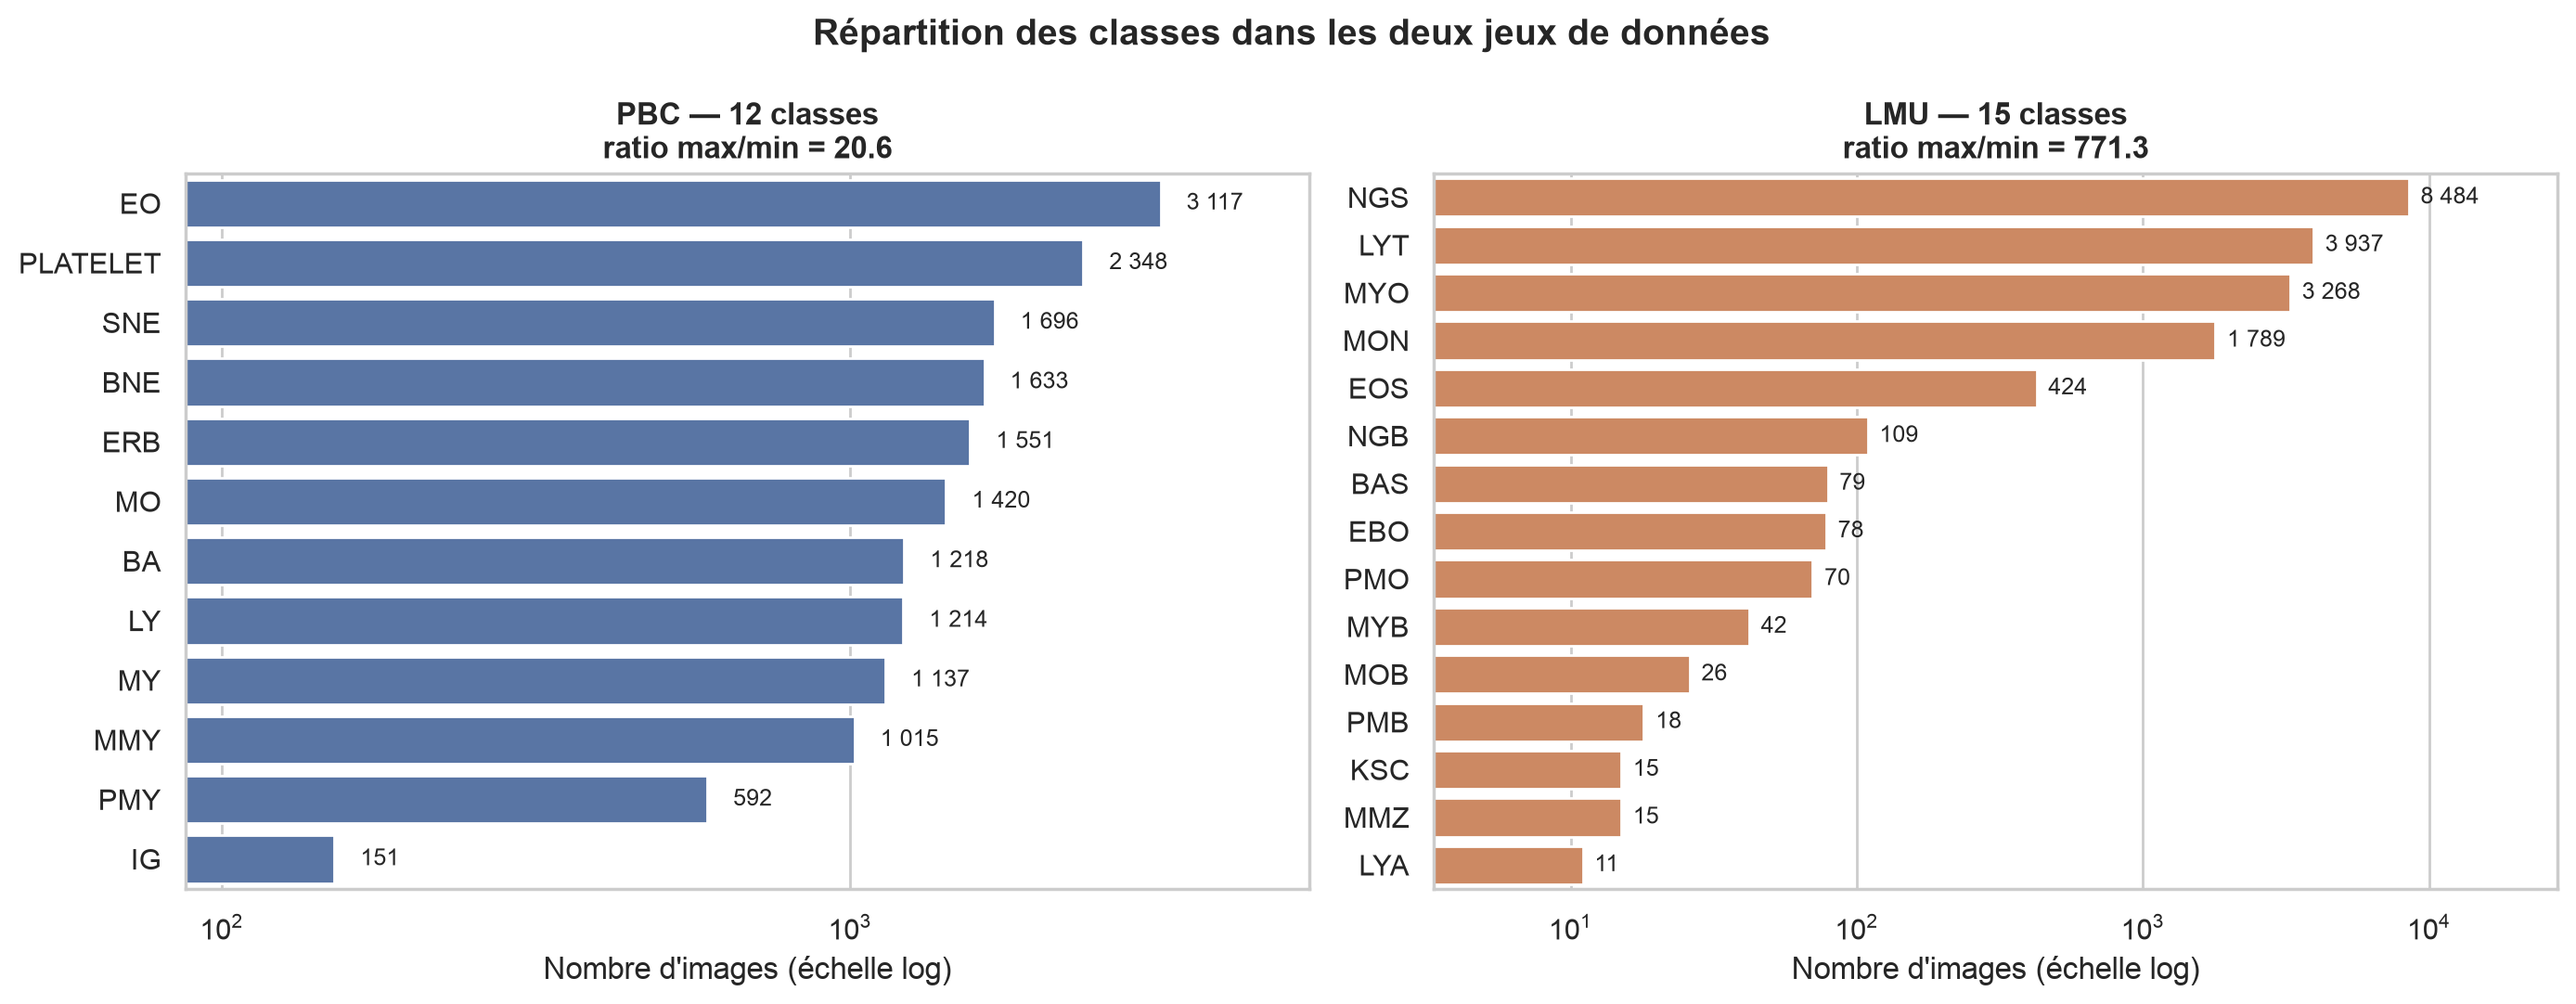
\includegraphics[width=\linewidth]{report/repartition_classes.png}
  \caption{Répartition des classes dans les deux jeux de données (échelle logarithmique).}
  \label{fig:repartition-classes}
\end{figure}

Ce déséquilibre appelle plusieurs pistes de rééquilibrage, à n’appliquer qu’au jeu d’entraînement afin de ne pas biaiser l’évaluation : le regroupement de classes proches (par exemple les lymphocytes atypiques, très peu nombreux, avec les lymphocytes typiques), la suppression des classes à très faible effectif ou sans intérêt clinique, le rééchantillonnage des classes minoritaires, ou encore la pondération des classes dans la fonction de perte.

\subsubsection*{Comparaison visuelle des classes et des sources}

Une comparaison d’une image par classe permet d’observer à la fois les différences morphologiques entre types cellulaires et les différences de rendu entre les deux sources.
Les images PBC et LMU se distinguent nettement à l’\oe{}il, par leur cadrage, leur coloration et leur fond.

\begin{figure}[H]
  \centering
  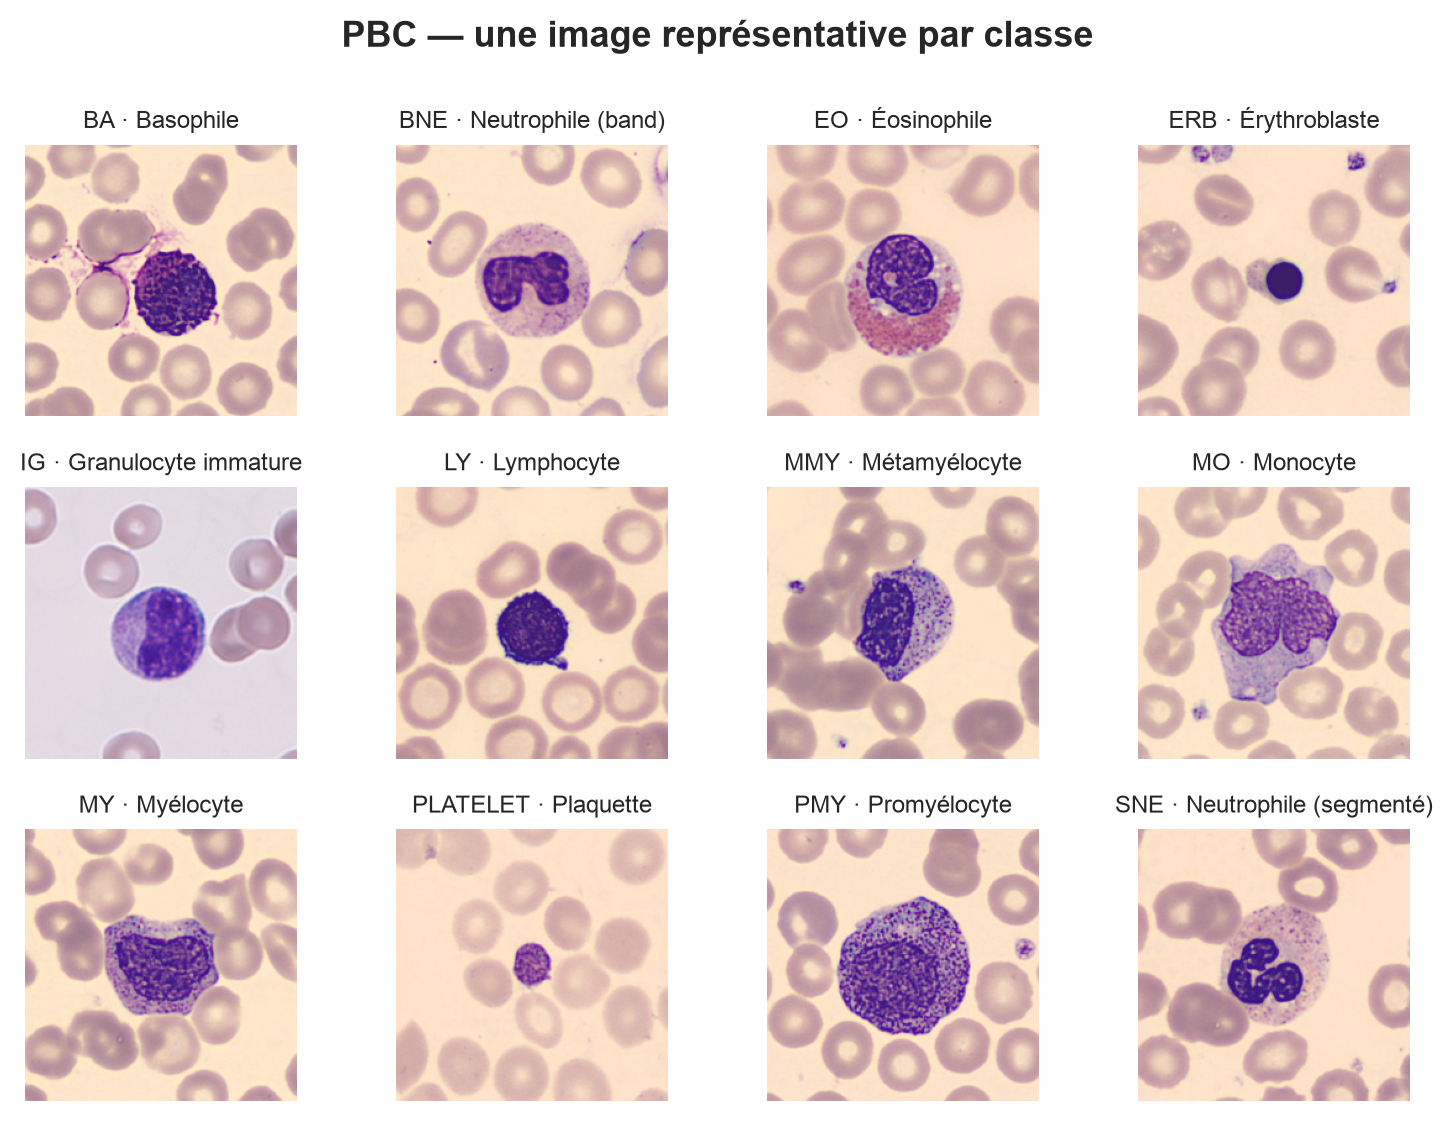
\includegraphics[width=0.78\linewidth]{report/mosaique_classes_pbc.png}\\[8pt]
  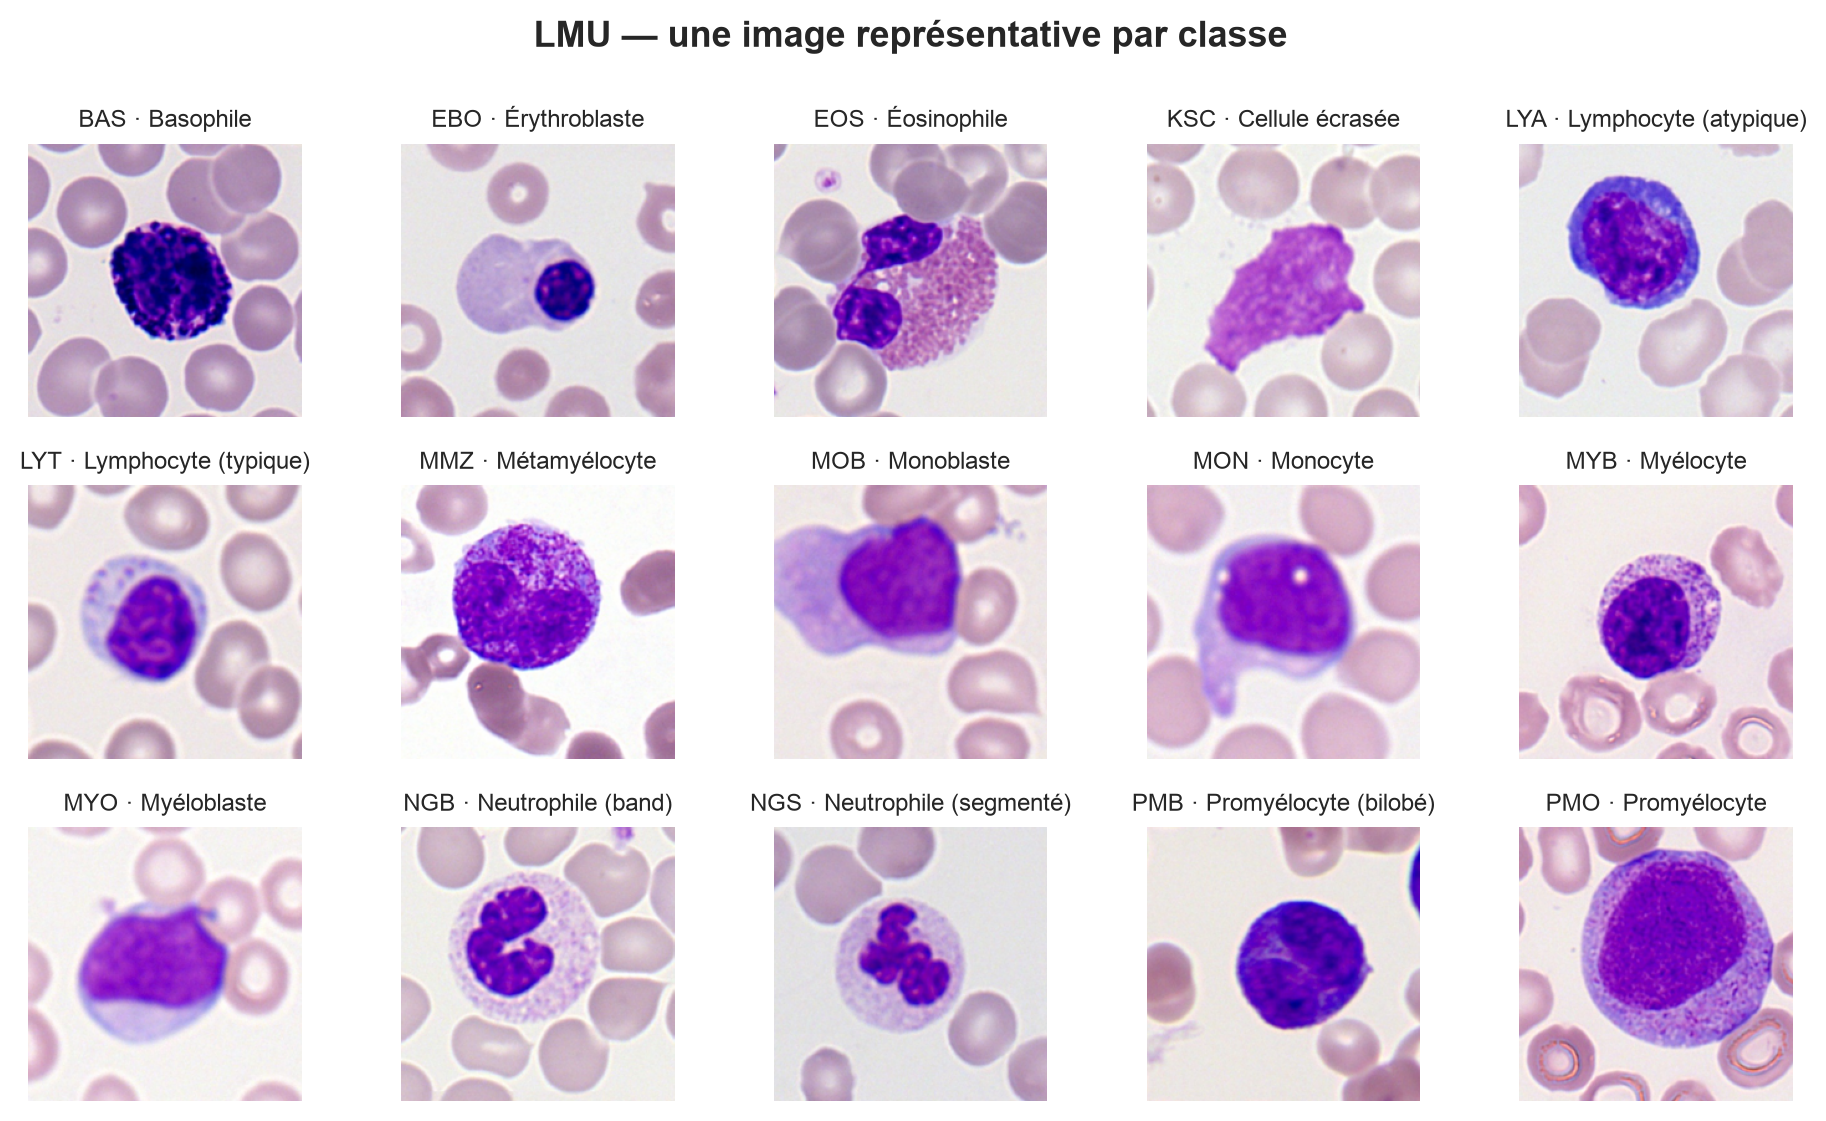
\includegraphics[width=0.78\linewidth]{report/mosaique_classes_lmu.png}
  \caption{Une image représentative par classe, pour chaque source.
Les différences de cadrage, de coloration et de fond entre PBC et LMU sont visibles au premier coup d’\oe{}il.}
  \label{fig:mosaique-classes}
\end{figure}

\subsubsection*{Distributions colorimétriques}

L’analyse des histogrammes de pixels confirme ces différences (figure~\ref{fig:histogrammes-rgb}).
Les distributions des canaux \textbf{R}, \textbf{G} et \textbf{B}, ainsi que celles des niveaux de gris, varient nettement selon le dataset : le pic clair des images PBC est plus haut et plus resserré, celui de LMU plus étalé et légèrement décalé.
Elles varient aussi selon le type cellulaire (figure~\ref{fig:histogrammes-type}).
Ces distributions constituent des variables explicatives potentielles pour un modèle, mais peuvent aussi encoder une information liée à la source d’acquisition plutôt qu’à la morphologie de la cellule.

\begin{figure}[H]
  \centering
  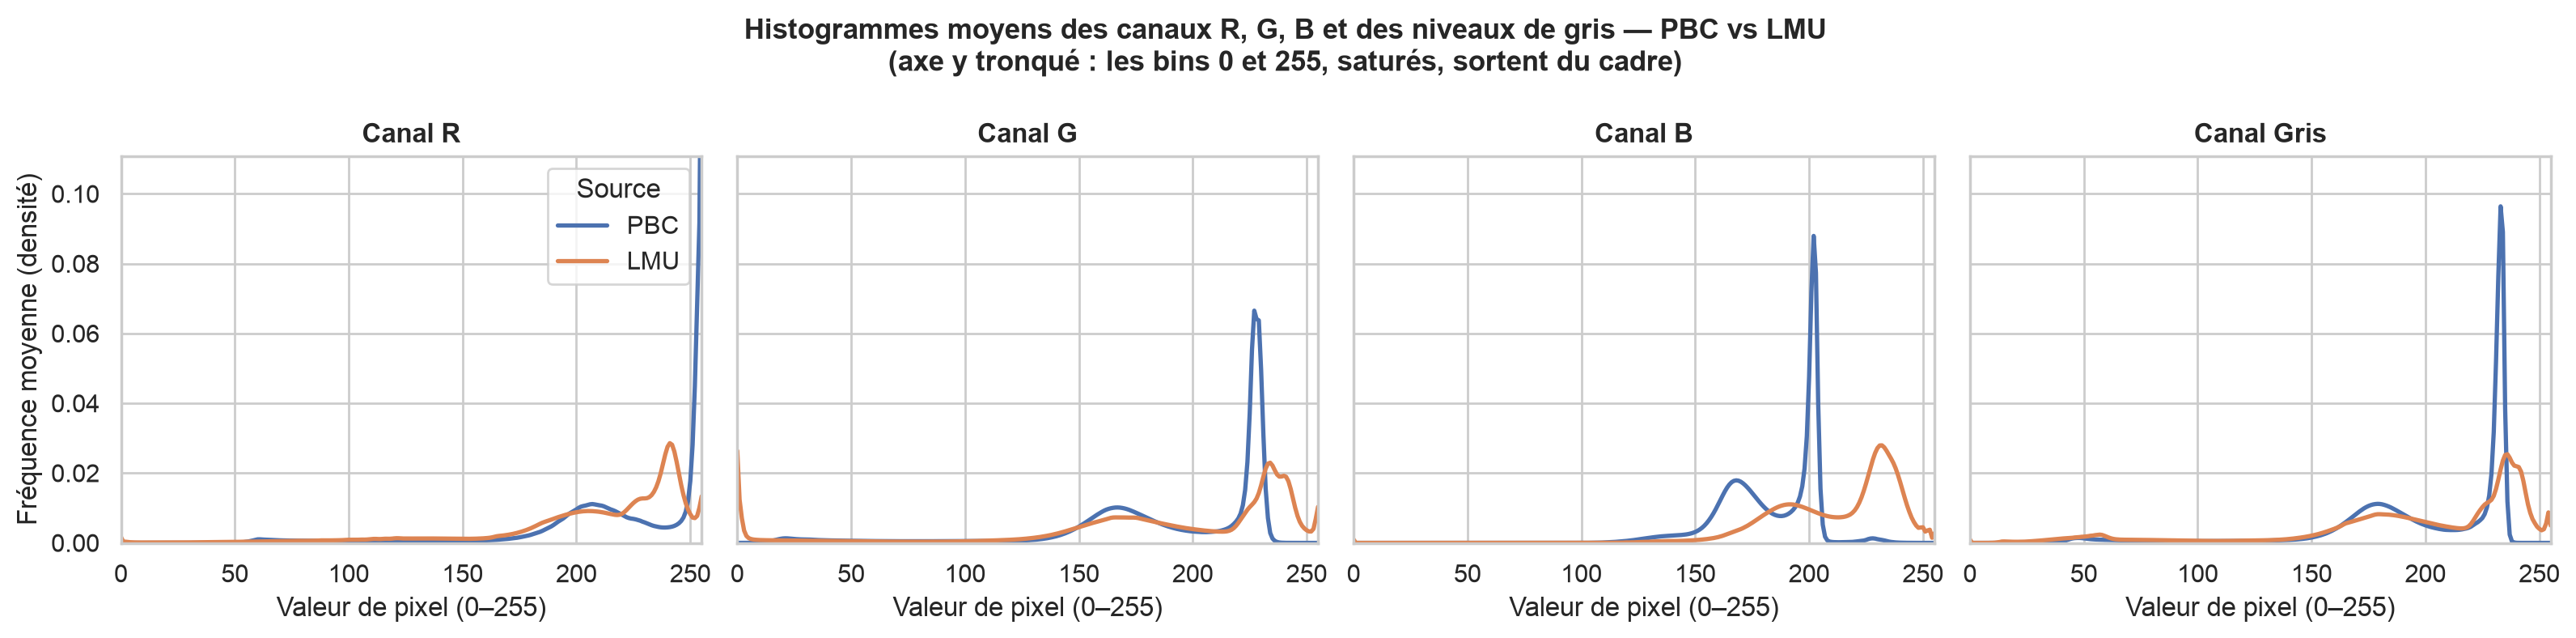
\includegraphics[width=\linewidth]{report/histogrammes_rgb.png}
  \caption{Histogrammes moyens des canaux R, G, B et des niveaux de gris, PBC contre LMU.}
  \label{fig:histogrammes-rgb}
\end{figure}

\begin{figure}[H]
  \centering
  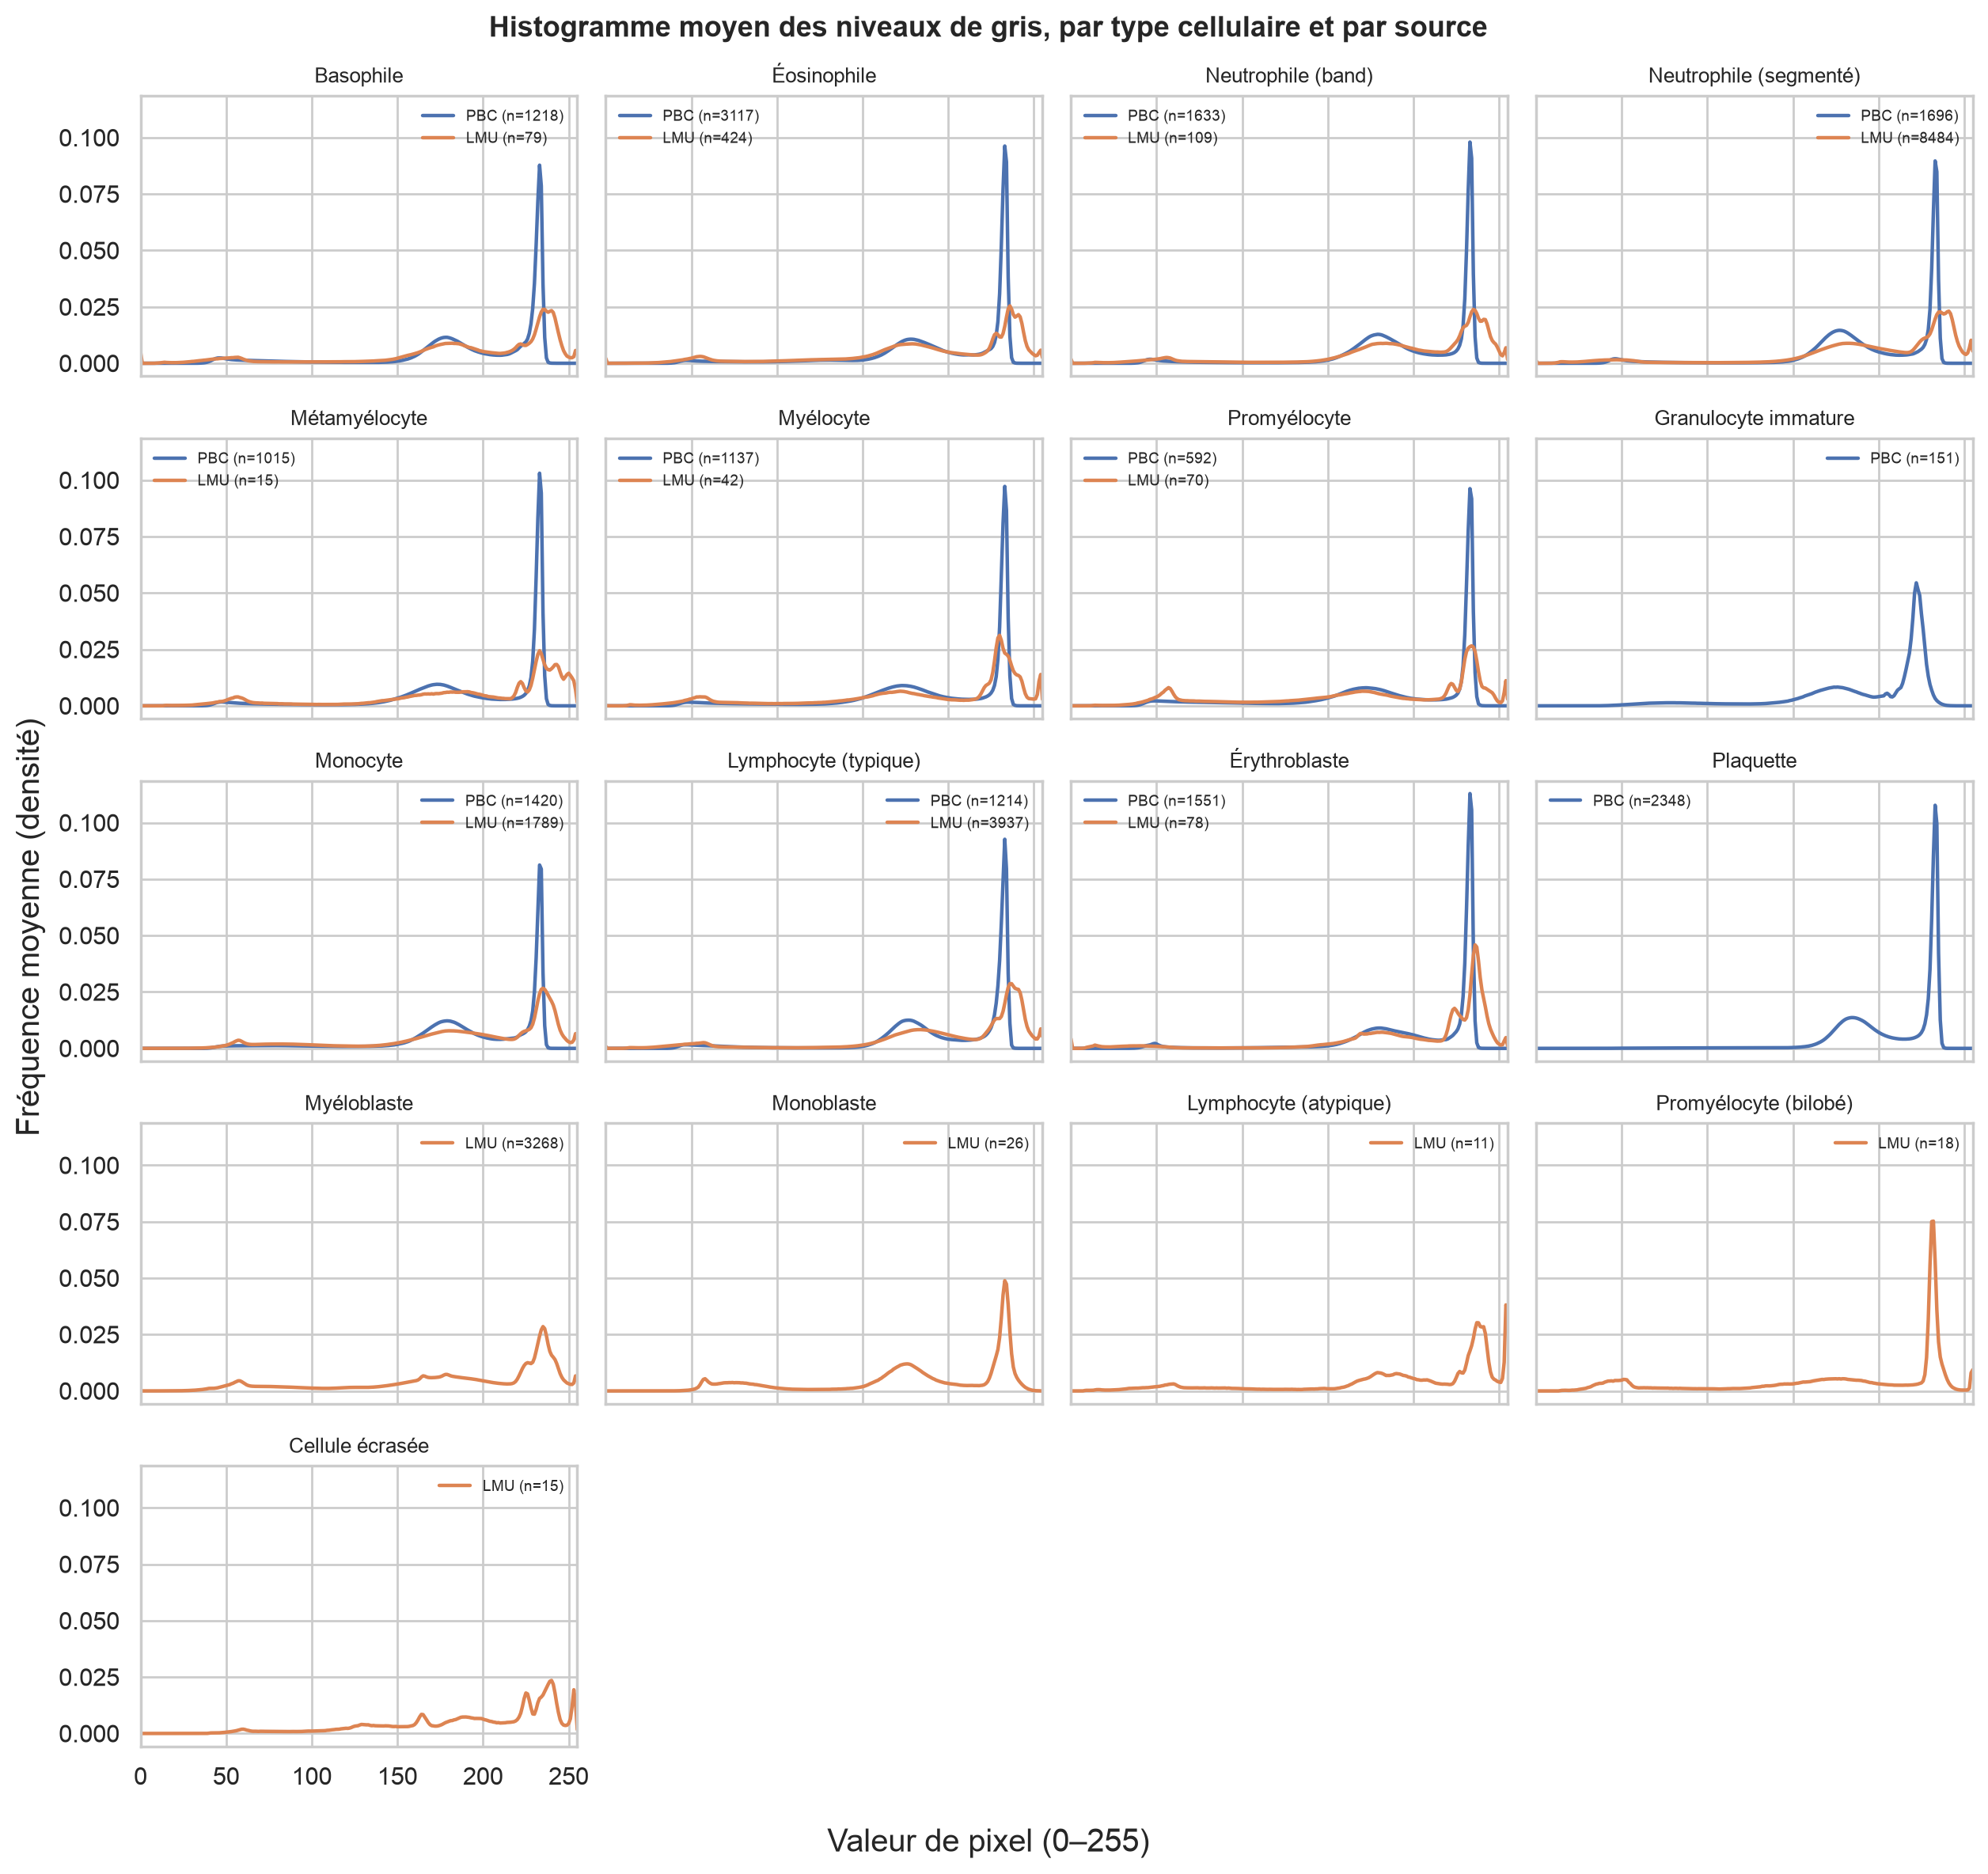
\includegraphics[width=0.9\linewidth]{report/histogrammes_rgb_par_type.png}
  \caption{Histogramme moyen des niveaux de gris décliné par type cellulaire et par source.
L’écart PBC/LMU se retrouve dans presque toutes les classes.}
  \label{fig:histogrammes-type}
\end{figure}

Pour quantifier ces écarts, trois indicateurs synthétiques ont été calculés : \textbf{luminosité moyenne}, \textbf{contraste} et \textbf{netteté}.
La luminosité moyenne est proche entre les deux sources, mais le \textbf{contraste} est systématiquement plus élevé et plus dispersé dans LMU (figure~\ref{fig:luminosite-contraste}) ; ces indicateurs varient également selon la classe cellulaire.

\begin{figure}[H]
  \centering
  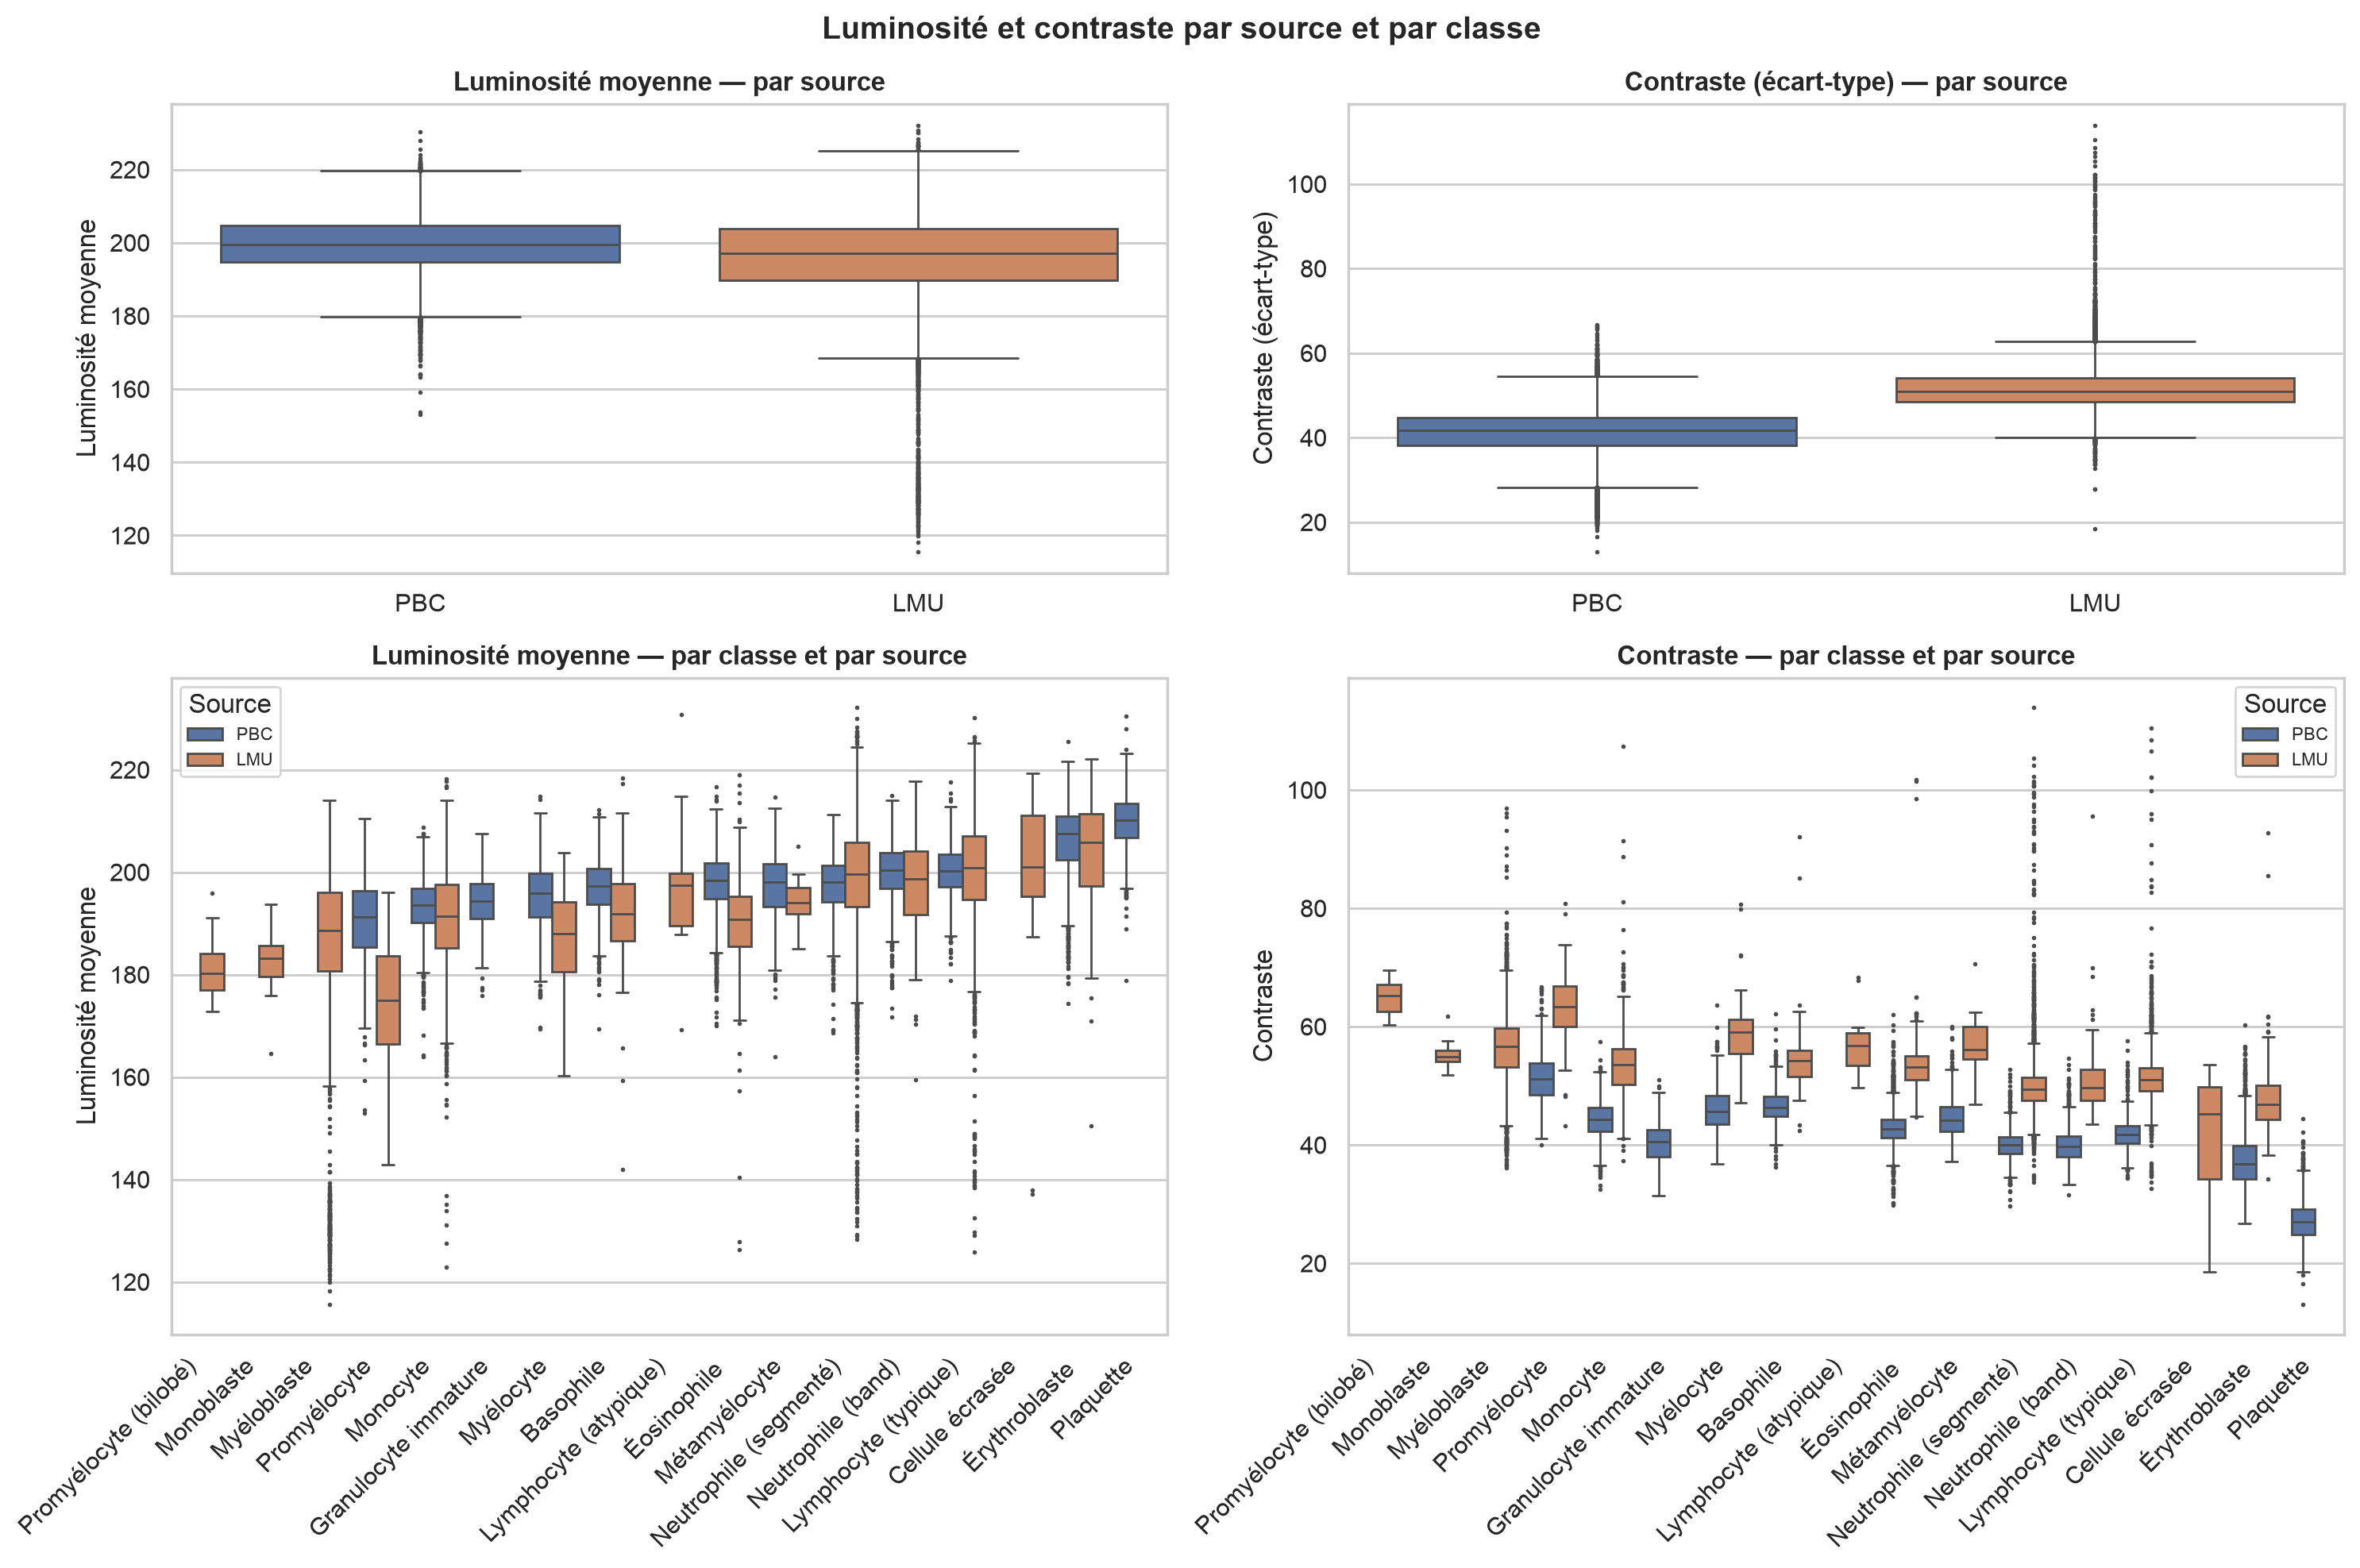
\includegraphics[width=\linewidth]{report/luminosite_contraste.png}
  \caption{Luminosité et contraste, par source (haut) et par classe et par source (bas).}
  \label{fig:luminosite-contraste}
\end{figure}

\subsubsection*{Netteté et images potentiellement floues}

La netteté, mesurée par la variance du Laplacien, permet d’identifier les images présentant un possible défaut de mise au point.
Sa distribution est globalement plus élevée pour PBC que pour LMU (figure~\ref{fig:nettete}).
En retenant le \textbf{2\textsuperscript{e} percentile} de chaque source comme seuil de contrôle (netteté $\approx$ 20 pour PBC, $\approx$ 15 pour LMU), une quarantaine d’images sur 2\,000 par source sont signalées comme potentiellement floues (souvent des plaquettes ou de petites cellules pour PBC).
Ces observations sont des points à vérifier, sans être automatiquement écartées.

\begin{figure}[H]
  \centering
  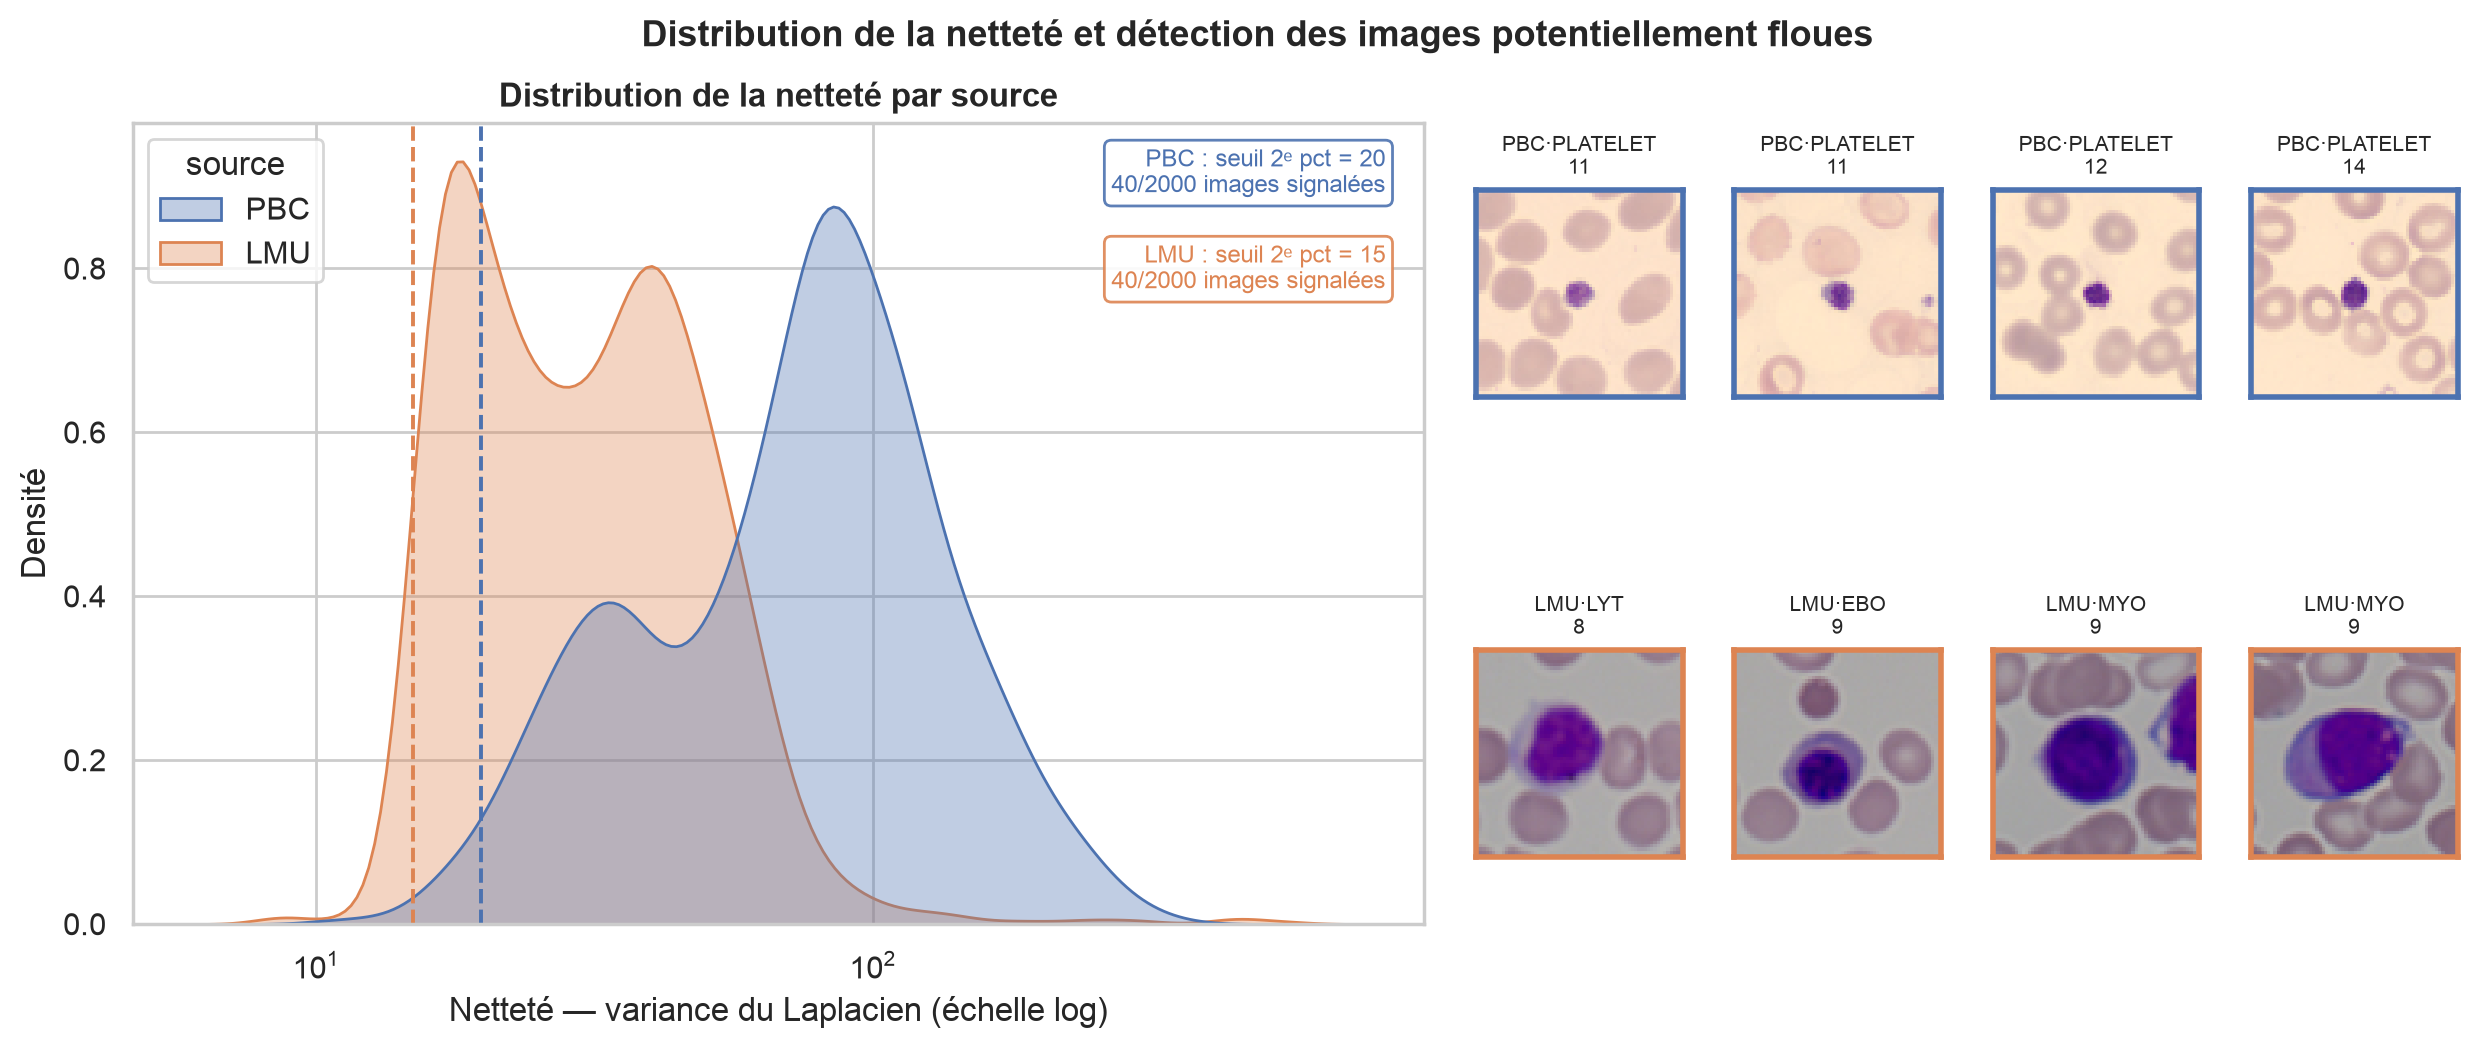
\includegraphics[width=\linewidth]{report/nettete.png}
  \caption{Distribution de la netteté par source et vignettes des images les moins nettes de l’échantillon.}
  \label{fig:nettete}
\end{figure}

\subsubsection*{Format, taille et poids des images}

Les caractéristiques techniques des fichiers diffèrent fortement selon la source (figure~\ref{fig:format-images}).
Les images LMU sont encodées en \textbf{TIFF sans perte}, toutes en \textbf{400 $\times$ 400 pixels} et sur quatre canaux (RGBA : le canal alpha doit être retiré explicitement à la lecture, faute de quoi certaines images sont chargées avec un fond noir).
Les images PBC sont en \textbf{JPEG}, sur trois canaux RGB, et en \textbf{360 $\times$ 363 pixels} pour la quasi-totalité (quelques centaines en 360 $\times$ 360 ou 366 $\times$ 369).
Le poids des fichiers s’en ressent directement : une médiane d’environ \textbf{625 Ko} par image TIFF, contre \textbf{16 Ko} pour les JPEG, soit un facteur \textbf{$\approx$ 40}.

\begin{figure}[H]
  \centering
  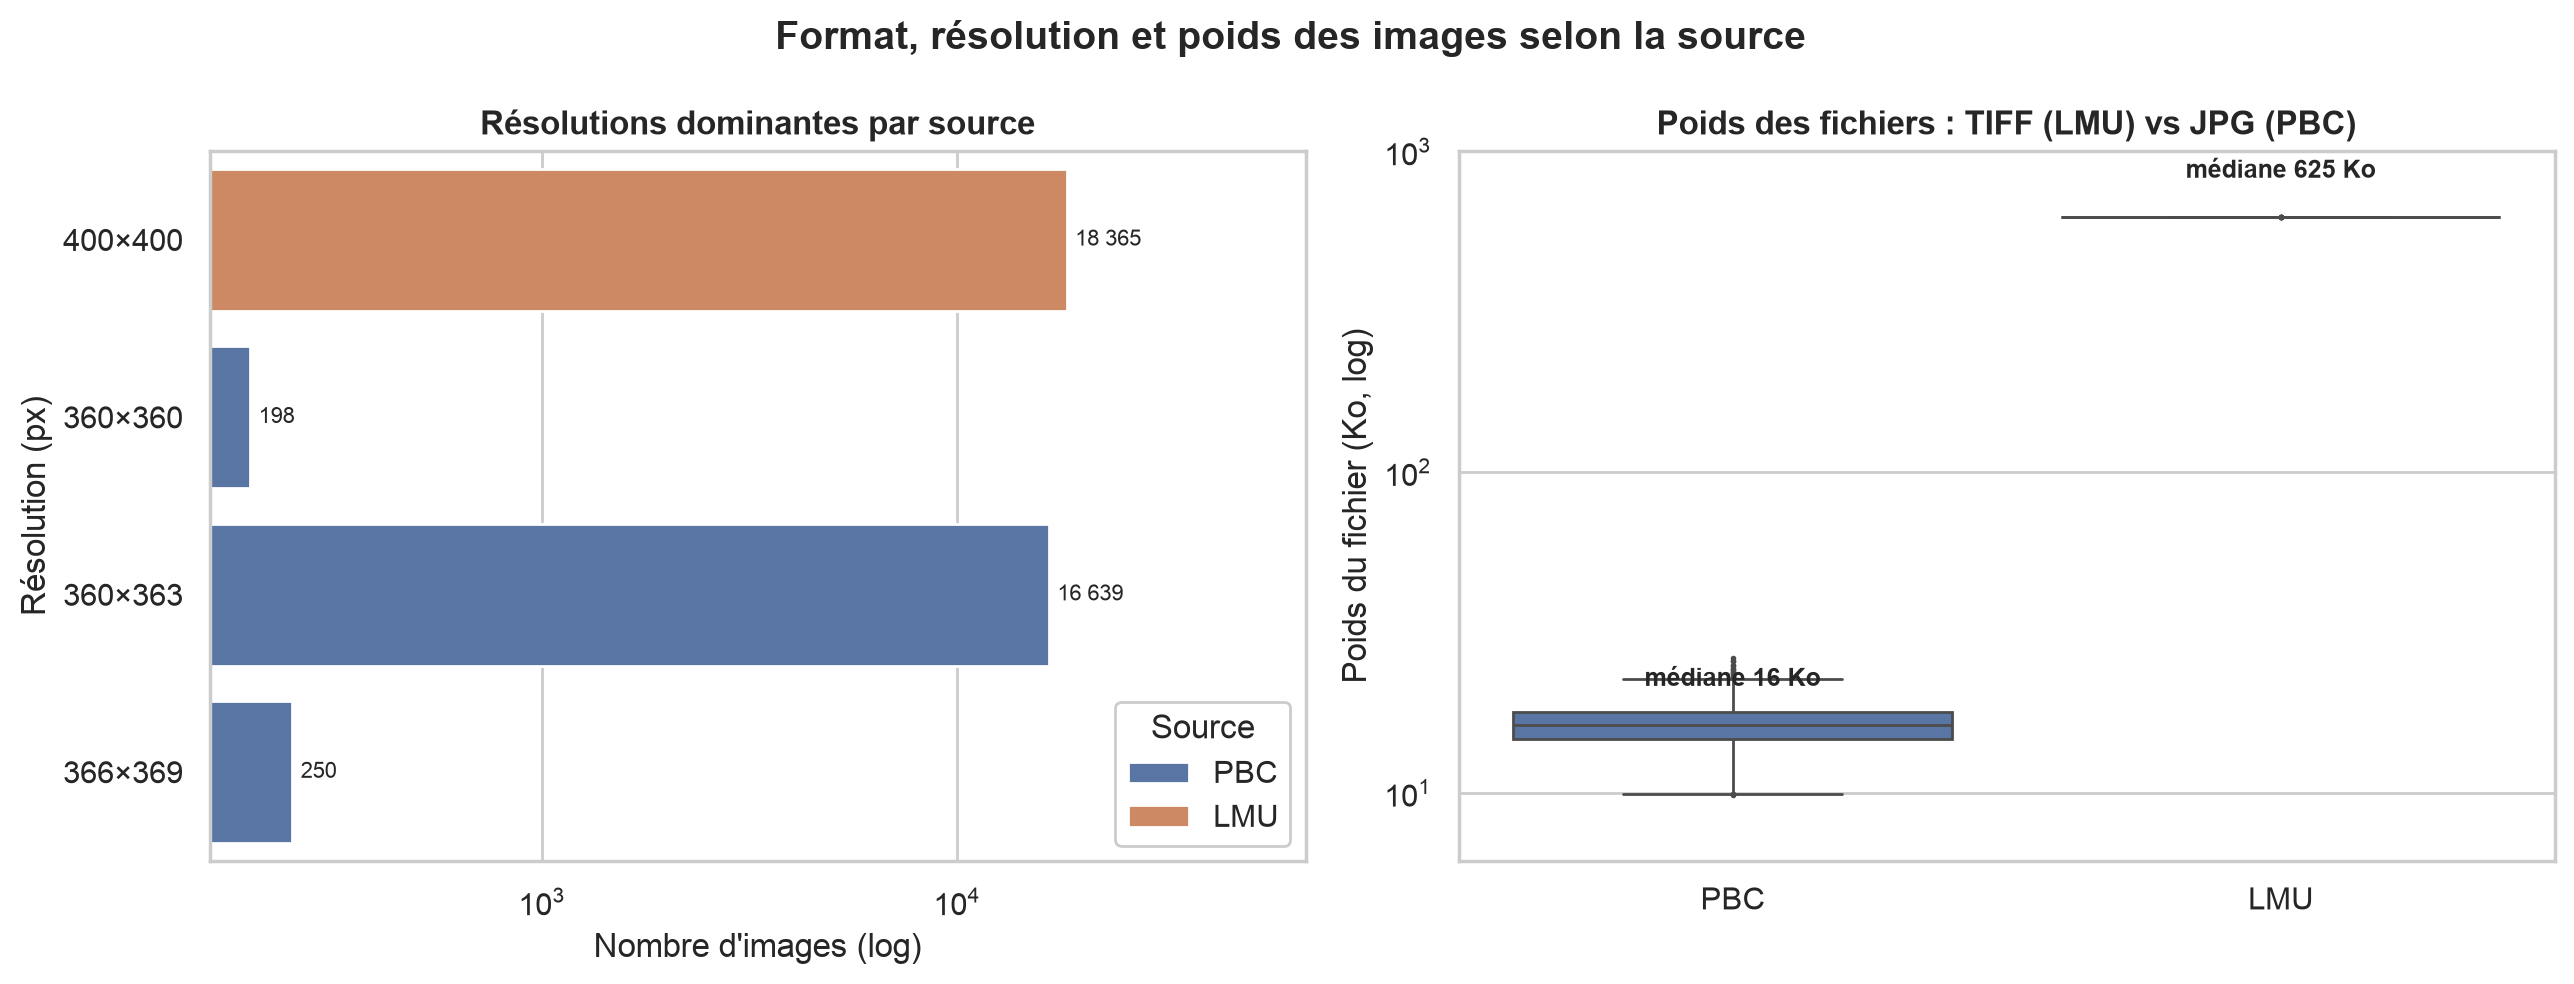
\includegraphics[width=\linewidth]{report/format_images.png}
  \caption{Résolutions dominantes (gauche) et poids des fichiers en échelle logarithmique (droite), par source.}
  \label{fig:format-images}
\end{figure}

\label{par:jpeg-artefacts}La compression JPEG des images de Barcelone est le point le plus problématique.
Étant une compression avec pertes, elle laisse dans l’image des \textbf{artefacts caractéristiques} que les TIFF de Munich n’ont pas, par exemple un découpage en blocs de 8 $\times$ 8 pixels.
Ces artefacts ne sont présents que d’un seul côté du corpus : « présence ou absence de blocs 8 $\times$ 8 » devient alors un indicateur de site quasi parfait, qu’un réseau convolutif, qui est fait pour détecter ce genre de motif local et périodique, peut apprendre à la place de la morphologie cellulaire.
Le raccourci est d’autant plus pernicieux qu’il est invisible à l’\oe{}il, qu’il ne dépend pas du contenu de l’image et qu’il survit à la plupart des normalisations colorimétriques.

Plus généralement, résolution, artefacts de compression, bordures et dynamique des pixels forment un ensemble de régularités de bas niveau qui offrent au modèle autant de moyens de prédire la source plutôt que le type cellulaire, ce qui dégrade la généralisation.
Une analyse en composantes principales (PCA) réalisée sur un échantillon d’images confirme ce point : les images se regroupent d’abord selon leur source.

\begin{figure}[H]
  \centering
  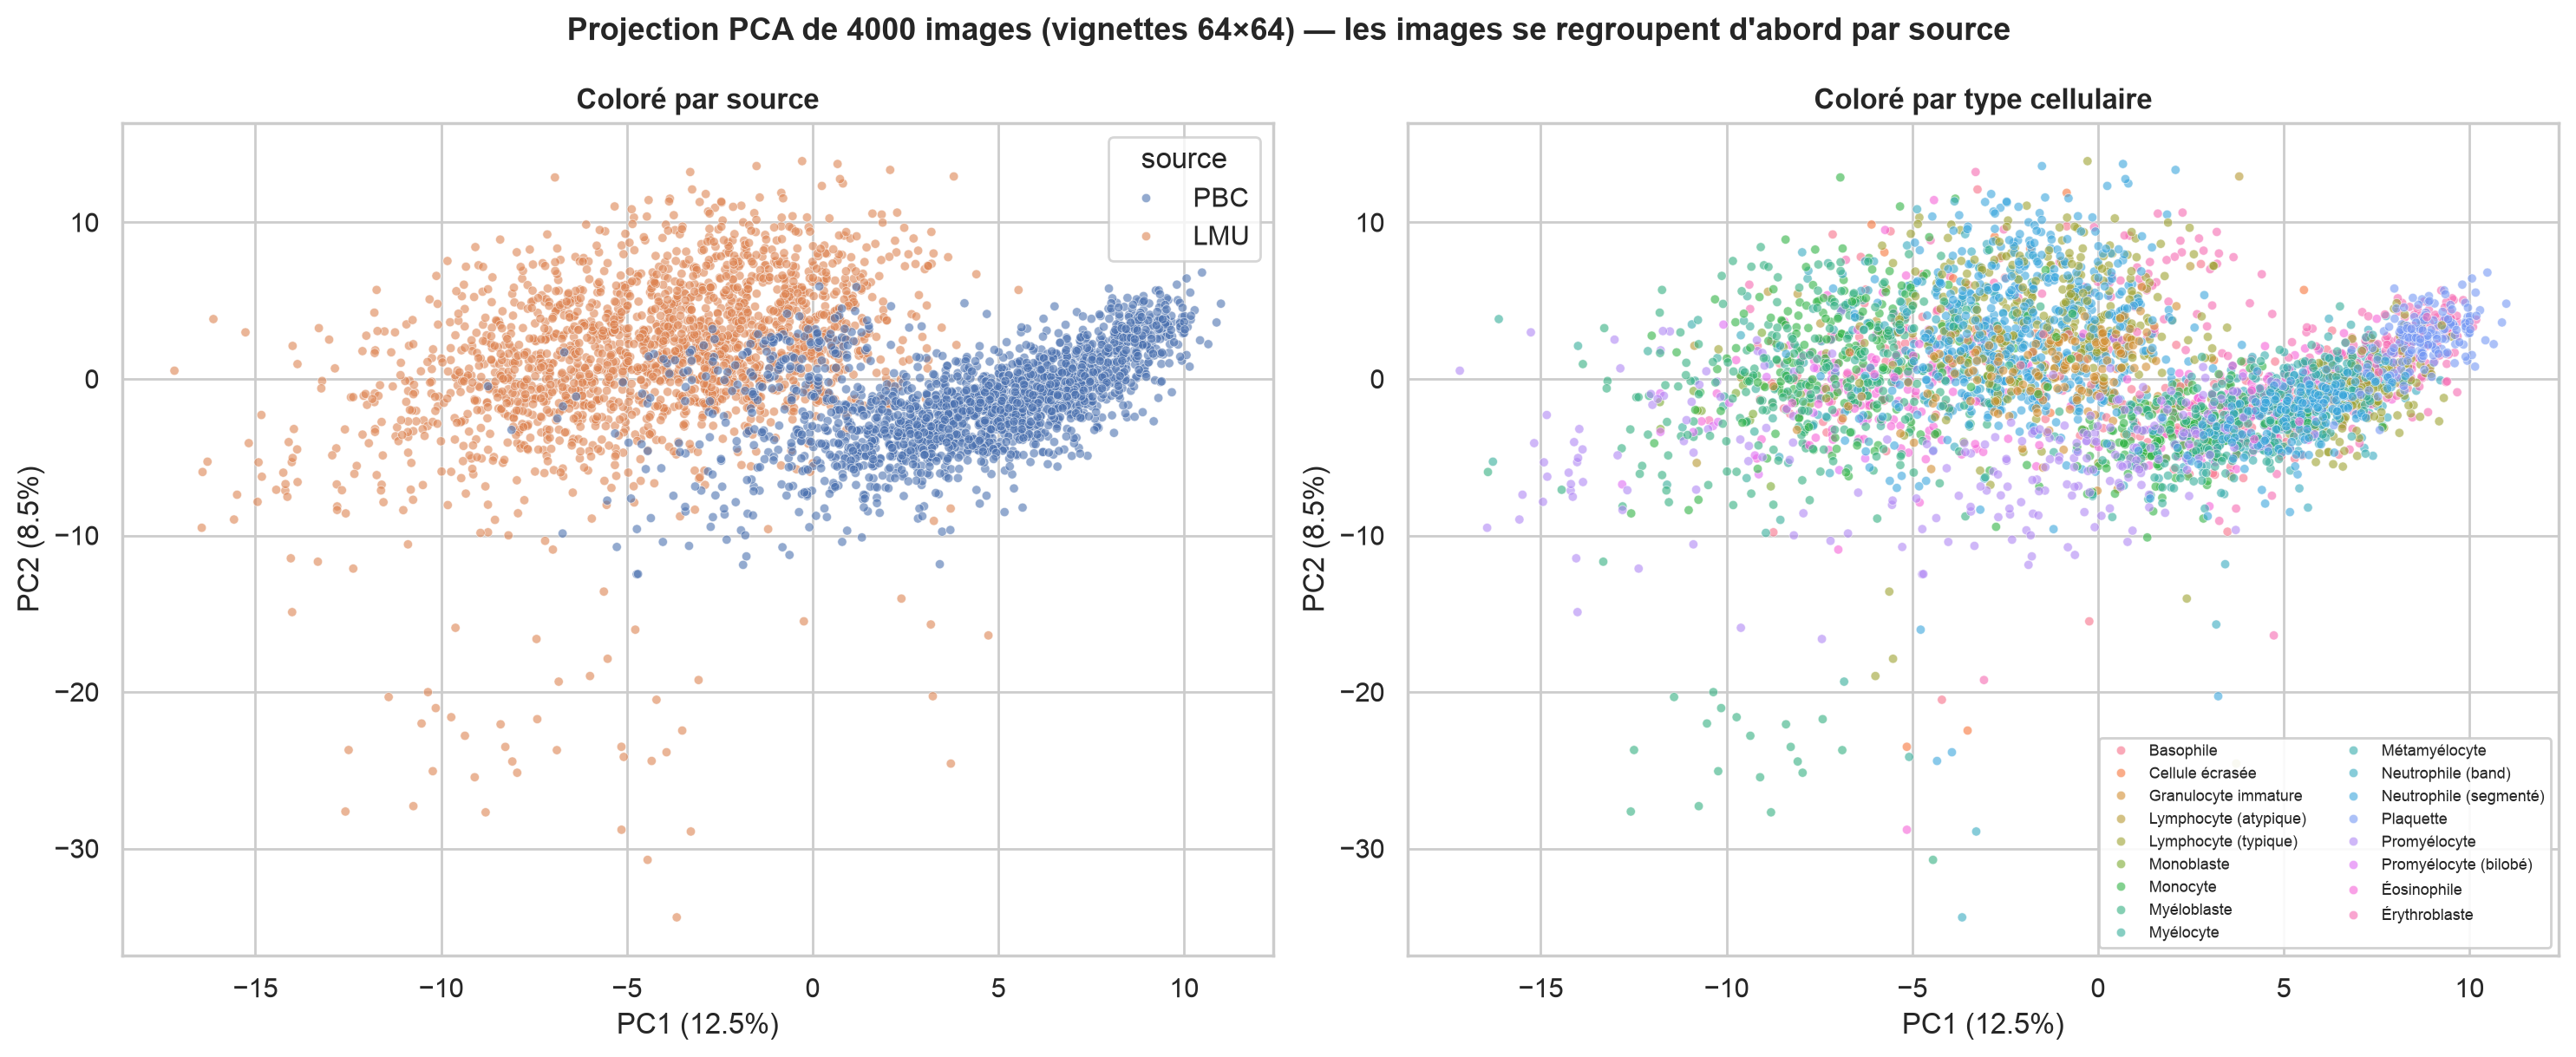
\includegraphics[width=\linewidth]{report/pca_source.png}
  \caption{Projection PCA d’un échantillon d’images (vignettes 64 $\times$ 64).
Colorée par source (gauche), les deux nuages se séparent le long de la première composante ; colorée par type cellulaire (droite), aucune structure nette n’apparaît.}
  \label{fig:pca-source}
\end{figure}

\subsubsection*{Synthèse}

Le tableau~\ref{tab:synthese-sources} récapitule les principales différences observées entre les deux sources.

\begin{table}[H]
  \centering
  \begin{tabular}{lll}
    \toprule
    \textbf{Caractéristique} & \textbf{PBC (Barcelone)} & \textbf{LMU (Munich)} \\
    \midrule
    Nombre d’images        & 17\,092                & 18\,365 \\
    Nombre de classes      & 12 (13 étiquettes)     & 15 \\
    Déséquilibre (max/min) & 20,6 (2,7 par groupe)  & 771,3 \\
    Résolution dominante   & 360 $\times$ 363 px    & 400 $\times$ 400 px \\
    Format / poids médian  & JPEG, $\approx$ 16 Ko  & TIFF, $\approx$ 625 Ko \\
    Canaux                 & 3 (RGB)                & 4 (RGBA) \\
    Population             & individus sains        & 100 patients LMA + 100 témoins \\
    \bottomrule
  \end{tabular}
  \caption{Synthèse des différences entre les deux sources de données.}
  \label{tab:synthese-sources}
\end{table}

Ces observations orientent la modélisation sur trois points : contrôler le déséquilibre du jeu d’apprentissage, limiter l’information de source portée par la colorimétrie, le contraste et les artefacts de compression, et vérifier la qualité des données en écartant ou en contrôlant les images problématiques.
Plusieurs pistes visant à atténuer ces problèmes ont été implémentés et seront décrits dans la section \ref{sec:pre-processing-feature-engineering}.
L’enjeu de la modélisation sera d’évaluer dans quelle mesure ces caractéristiques influencent réellement la capacité d’un CNN à distinguer les différentes populations cellulaires.


\subsection{Pre-processing et feature engineering}
\label{sec:pre-processing-feature-engineering}
\subsubsection{Fusion des datasets}

Pour exploiter les deux sources conjointement, il faut d’abord ramener leurs nomenclatures (13 étiquettes pour PBC, 15 classes pour LMU ; tableaux~\ref{tab:types-pbc} et~\ref{tab:types-lmu}) à une \textbf{taxonomie commune}.
Le principe retenu est de regrouper le plus largement possible entre les deux sites, de ne conserver un niveau de détail fin que lorsqu’il est cliniquement justifié, et de n’écarter qu’une seule catégorie qui n’est pas un véritable type cellulaire.
On aboutit à \textbf{10 classes entraînables} (plus une catégorie exclue), pour un total inchangé de \textbf{35\,457 images} : aucune image n’est perdue dans l’opération.
Le tableau~\ref{tab:fusion-taxonomie} détaille la correspondance.

\begin{table}[H]
  \centering
  \small
  \setlength{\tabcolsep}{4pt}
  \renewcommand{\arraystretch}{1.2}
  \begin{tabular}{@{}>{\raggedright\arraybackslash}p{2.3cm} >{\raggedright\arraybackslash}p{4.2cm} >{\raggedright\arraybackslash}p{2.9cm} r >{\raggedright\arraybackslash}p{2.0cm}@{}}
    \toprule
    \textbf{Classe finale} & \textbf{Étiquettes PBC} & \textbf{Étiquettes LMU} & \textbf{Total} & \textbf{Criticité} \\
    \midrule
    Neutrophile            & BNE, SNE, NEUTROPHIL (3\,329) & NGB, NGS (8\,593) & 11\,922 & Normal \\
    Lymphocyte             & LY (1\,214)                   & LYT, LYA (3\,948) & 5\,162  & Normal \\
    Éosinophile            & EO (3\,117)                   & EOS (424)         & 3\,541  & Normal \\
    Monocyte               & MO (1\,420)                   & MON (1\,789)      & 3\,209  & Normal \\
    Plaquette              & PLATELET (2\,348)             & Aucune            & 2\,348  & Normal \\
    Basophile              & BA (1\,218)                   & BAS (79)          & 1\,297  & Normal \\
    Érythroblaste          & ERB (1\,551)                  & EBO (78)          & 1\,629  & Intermédiaire \\
    Granulocytes immatures & MMY, MY, IG (2\,303)          & MYB, MMZ (57)     & 2\,360  & Intermédiaire \\
    Promyélocyte           & PMY (592)                     & PMB, PMO (88)     & 680     & \textbf{Critique} \\
    Blaste                 & Aucune                        & MYO, MOB (3\,294) & 3\,294  & \textbf{Critique} \\
    \midrule
    \emph{Smudge} (exclue) & Aucune                        & KSC (15)          & 15      & \textit{Non applicable} \\
    \bottomrule
  \end{tabular}
  \caption{Correspondance entre les étiquettes brutes des deux sources et la taxonomie fusionnée (10 classes entraînables, plus la catégorie \emph{smudge} exclue).
Effectifs entre parenthèses.}
  \label{tab:fusion-taxonomie}
\end{table}

Trois décisions structurent cette fusion.

\textbf{Fusion du monoblaste dans les blastes.} Le monoblaste (LMU, 26 images) est cliniquement l’une des classes les plus critiques, marqueur de leucémie aiguë monoblastique ou myélomonocytaire, mais son effectif est trop faible pour constituer une classe entraînable, quel que soit le rééquilibrage appliqué.
Il est donc regroupé avec le myéloblaste (3\,268 images) dans une classe \emph{Blaste} : la distinction entre les deux est perdue, mais la capacité à détecter la présence d’un blaste, l’objectif clinique prioritaire, est préservée.

\textbf{Exclusion des cellules écrasées.} La catégorie \emph{smudge} (KSC, 15 images) n’est pas un type cellulaire mais un artefact d’étalement (leucocyte fragile éclaté).
Elle est retirée de la taxonomie de classification : elle relève d’un contrôle qualité en amont du pipeline, pas d’une sortie du modèle.

\textbf{Isolement du promyélocyte.} Plutôt qu’une classe « granulocytes immatures » unique regroupant promyélocytes, myélocytes et métamyélocytes (environ 3\,000 images), le promyélocyte est maintenu en classe propre (680 images).
Sa forme hypergranuleuse permet de diagnostiquer la leucémie aiguë promyélocytaire (LMA-3), une urgence hématologique (risque de coagulation intravasculaire disséminée), un cran de gravité au-dessus du simple « virage à gauche » que traduisent myélocyte et métamyélocyte.
L’étiquette générique \texttt{IG} de PBC (151 images, non sous-typée) est en revanche rattachée par prudence au groupe myélocyte / métamyélocyte.

Deux classes restent par ailleurs \textbf{mono-site} : les plaquettes ne proviennent que de PBC, les blastes que de LMU.
Comme ce sont aussi les deux extrêmes de l’échelle de criticité, le risque qu’un modèle apprenne un raccourci « site d’acquisition » plutôt qu’une morphologie y est particulièrement sensible : une normalisation de coloration inter-sites et un test de contrôle « PBC contre LMU » sont nécessaires avant l’entraînement final.

\paragraph{Criticité clinique.} En complément du type cellulaire, la fusion définit une seconde variable cible : un \textbf{niveau de criticité} en trois paliers, destiné à prioriser la relecture humaine.
\begin{itemize}
  \item \textbf{Critique} (blaste, promyélocyte ; 3\,974 images) : marqueurs directs d’une leucémie aiguë ; un faux négatif constitue un raté diagnostique majeur.
  \item \textbf{Intermédiaire} (granulocytes immatures, érythroblaste ; 3\,989 images) : cellules anormales en sang périphérique mais non malignes par nature (virage à gauche, stress médullaire) ; un faux négatif est un signal clinique manqué, moins urgent.
  \item \textbf{Normal} (neutrophile, lymphocyte, éosinophile, monocyte, plaquette, basophile ; 27\,479 images) : cellules matures normales, pour lesquelles aucune sur-pondération n’est nécessaire.
\end{itemize}
Ce découpage servira de base pour pénaliser les erreurs selon leur gravité clinique plutôt que de traiter uniformément toutes les classes rares.

\subsubsection{Transformation et data augmentation des images}
\label{sub:transfo}

L’exploration a montré que le \textbf{site d’acquisition} est trivialement identifiable à partir des statistiques bas niveau de l’image (résolution, artefacts de compression, teinte du fond, contraste).
Sans correction, un classifieur de type cellulaire risque de s’appuyer sur ce raccourci plutôt que sur la morphologie : un risque d’autant plus sérieux que deux classes sont mono-site (plaquettes à Barcelone, blastes à Munich).
Le traitement des images poursuit donc deux objectifs distincts :

\begin{enumerate}
  \item \textbf{harmoniser} les deux sources (taille, format, couleur, contraste, compression) par des transformations \emph{déterministes}, appliquées identiquement au train, à la validation et au test ;
  \item \textbf{augmenter} la variabilité du seul jeu d’entraînement (géométrie, photométrie) par des transformations \emph{aléatoires}, pour améliorer la généralisation et compenser le déséquilibre des classes rares.
\end{enumerate}

\paragraph{Évaluation de l’harmonisation : un CNN retrouve toujours la source.} Pour mesurer le biais de domaine résiduel après transformation, on entraîne un petit CNN à une tâche annexe : \textbf{prédire la source} (Barcelone contre Munich) à partir de l’image transformée.
Une harmonisation parfaite rendrait les deux sources indistinguables (précision de 0,5, le hasard) ; une précision élevée signale au contraire qu’un indice de site subsiste.

Un premier \emph{random search} avait produit une vingtaine de configurations à 0,5 de précision, d’abord prises pour des harmonisations réussies.
C’était un artefact : ces entraînements avaient \textbf{divergé} (pas d’apprentissage trop élevé, perte figée à $\ln 2 \approx 0{,}69$, modèle prédisant une classe constante), et non atteint l’indistinguabilité.
En relançant la recherche avec un pas d’apprentissage plus faible, $10^{-3}$ au lieu de $10^{-2}$, plus aucun effondrement et le constat s’inverse :

\begin{itemize}
  \item \textbf{aucune combinaison de transformations ne fait tomber la précision près du hasard} : elle reste comprise entre \textbf{0,87 et 1,00}, de médiane \textbf{0,99} ;
  \item les traitements colorimétriques n’aident pas : CLAHE et le ré-encodage JPEG laissent la médiane inchangée ; seule la normalisation Reinhard, poussée avec un flou gaussien agressif, fait ponctuellement descendre la précision vers 0,87, au prix d’une perte de détail qui rendrait la classification cellulaire elle-même impossible ;
  \item le CNN retrouve donc le site \textbf{quasi parfaitement quel que soit le prétraitement}.
Le biais de domaine est réel et \textbf{robuste}.
\end{itemize}

Un test statistique confirme formellement ce constat descriptif : sur les 200 configurations, la précision moyenne vaut 0,992 (écart-type 0,012, médiane 0,992), très loin du hasard.
Un test de Shapiro-Wilk rejette la normalité de cette distribution ($W = 0{,}52$, $p = 3{,}9 \times 10^{-23}$, plafonnée près de 1) : on complète donc le test $t$ à un échantillon ($H_0$ : précision $= 0{,}5$) par un test des rangs signés de Wilcoxon, non paramétrique.
Les deux rejettent $H_0$ sans ambiguïté ($t(199) = 566{,}7$, $p < 10^{-300}$ ; Wilcoxon $p = 2{,}2 \times 10^{-35}$), avec une taille d'effet considérable (Cohen's $d = 40{,}1$) : le biais de domaine détecté n'est donc pas un artefact d'échantillonnage, il est statistiquement présent dans la quasi-totalité des configurations testées.

Ce résultat ne condamne pas le pipeline d’harmonisation : il rapproche fortement les images \emph{à l’œil} (fonds, luminosité, contraste) et réduit leur séparabilité \emph{linéaire}. La PCA, qui isole nettement les deux sources sur les données brutes, ne les distingue d'ailleurs presque plus après transformation (figure~\ref{fig:pca-comparaison}).
Mais un réseau convolutif, non linéaire, exploite des indices plus fins (texture de la coloration, micro-artefacts) que ni Reinhard ni la compression ne suppriment.
La configuration retenue (\texttt{configs/dataset.yaml} : Reinhard, CLAHE, JPEG qualité 30, jitter modéré) correspond aux bonnes pratiques d’harmonisation inter-sites en pathologie computationnelle, où normalisation de coloration et augmentation sont jugées complémentaires \parencite{tellez2019quantifying} ; elle est conservée pour ces bénéfices, sans prétendre neutraliser le raccourci « site » pour un CNN.

La conséquence pour la modélisation porte sur deux points : (i) lire les métriques des classes mono-site (plaquette, blaste) avec prudence, car le modèle peut y réussir en devinant le site plutôt que la morphologie ; (ii) si le biais s’avère limitant, recourir à des méthodes qui l’attaquent directement (entraînement adversarial de domaine, \emph{fine-tuning} séparé par site), non testées ici.

\begin{figure}[H]
  \centering
  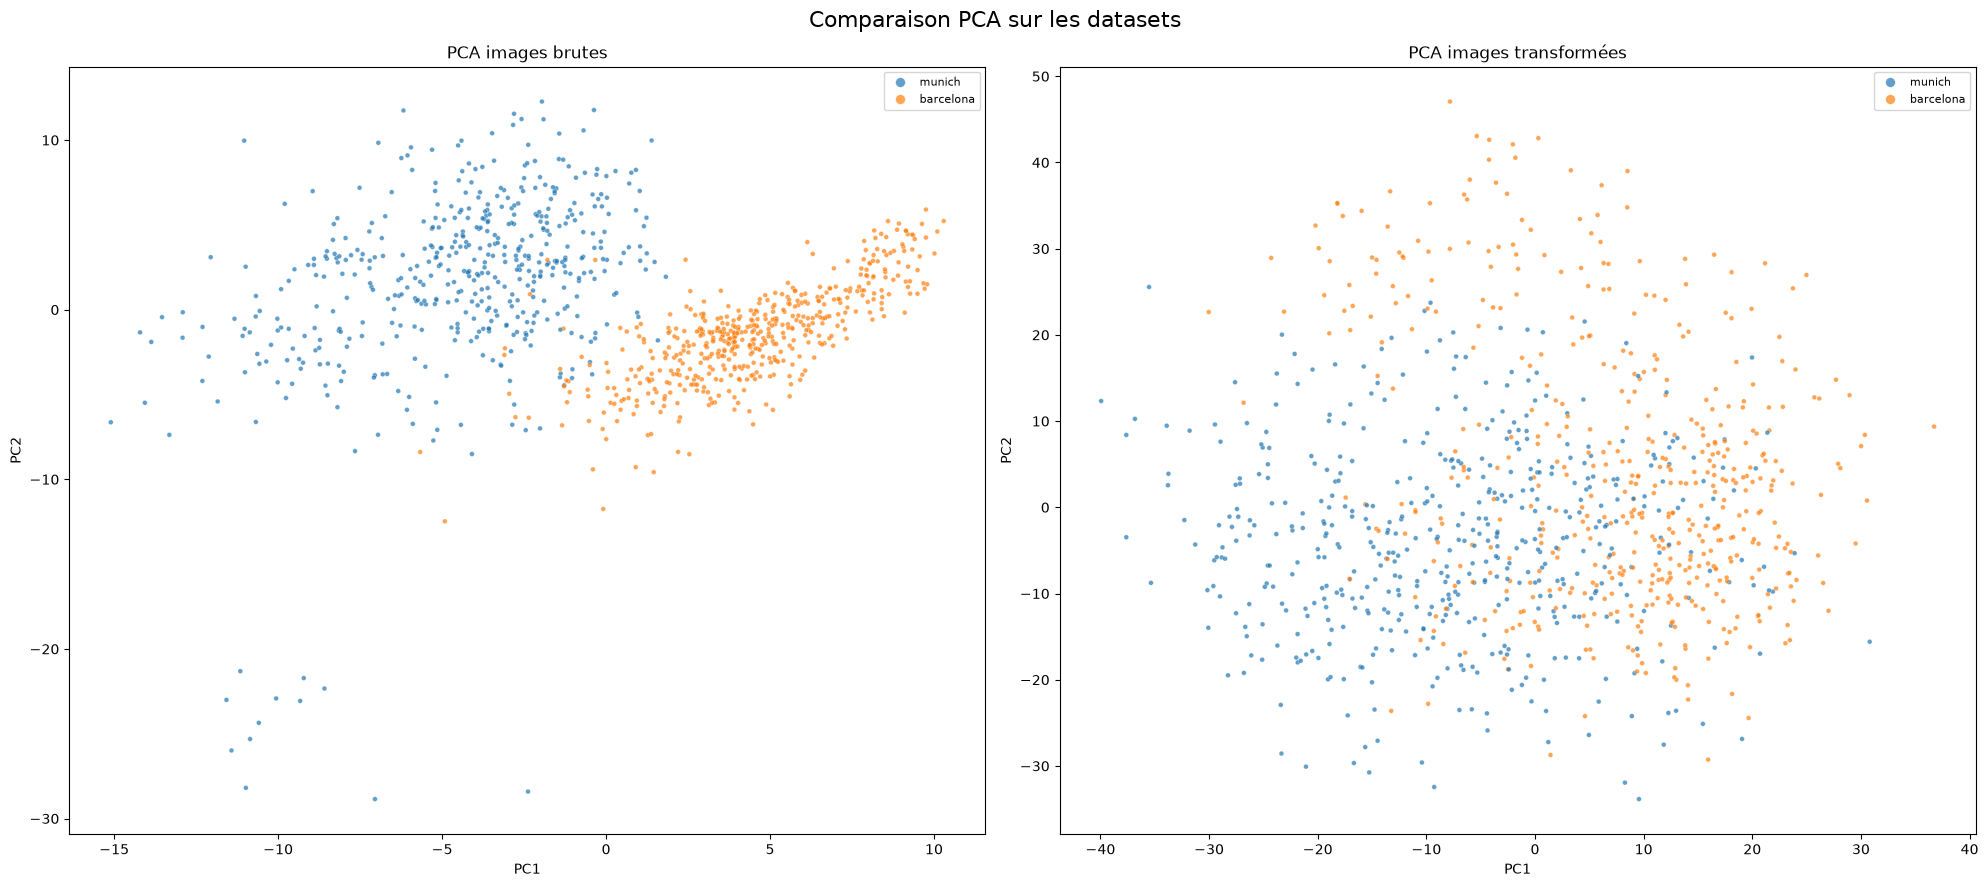
\includegraphics[width=\linewidth]{report/pca_comparaison.png}
  \caption{PCA d’un sous-échantillon d’images, avant (gauche) et après (droite) le pipeline d’harmonisation.
La séparation \emph{linéaire} nette des deux sources sur les données brutes s’efface presque après transformation. Un CNN, lui, continue de les distinguer.}
  \label{fig:pca-comparaison}
\end{figure}

\paragraph{Pipeline d’harmonisation.} Assemblé dans \texttt{build\_transform()} sous la forme d’un unique \texttt{Compose} (\texttt{torchvision.transforms.v2} \parencite{torchvision}), il enchaîne :

\begin{enumerate}
  \item \textbf{Redimensionnement avec \emph{padding}} en 224 $\times$ 224 : le ratio d’origine est conservé (pas de distorsion des cellules), le complément est rempli en blanc, cohérent avec le fond clair des lames.
Règle d’un coup l’écart de dimensions et de ratio.
  \item \textbf{Conversion en 3 canaux} (\texttt{convert("RGB")}) : retire le canal alpha des TIFF de Munich, sinon lus avec un fond noir.
  \item \textbf{Reinhard dans l’espace Lab} \parencite{reinhard2001colortransfer} (implémentation \texttt{torchstain} \parencite{torchstain}) : recale la moyenne et l’écart-type des canaux L, a et b vers une cible neutre, obtenue en moyennant les statistiques d’un échantillon tiré à parts égales entre les deux sites.
L’espace Lab découple la luminance de la chrominance, ce qui corrige la dérive de teinte du fond (chaud à Barcelone, froid à Munich) sans coupler artificiellement les canaux.
  \item \textbf{CLAHE sur le seul canal L} \parencite{zuiderveld1994clahe} (\texttt{kornia} \parencite{riba2020kornia}, \texttt{clip\_limit}~=~2, grille 8 $\times$ 8) : égalise le contraste local, plus élevé et plus dispersé à Munich, en bornant le gain pour ne pas sur-amplifier le bruit, contrairement à l’égalisation adaptative classique \parencite{pizer1987ahe}.
Les canaux a et b ne sont pas touchés, pour préserver la teinte des granulations, qui porte un signal diagnostique (orangé des éosinophiles, violet foncé des basophiles, azurophiles des promyélocytes).
  \item \textbf{Ré-encodage JPEG en qualité 30} : impose les mêmes artefacts de compression à toutes les images et supprime ainsi l’indice « présence ou absence de blocs 8 $\times$ 8 » décrit plus haut dans \hyperref[par:jpeg-artefacts]{Format, taille et poids des images}.
  \item \textbf{Centrage-réduction} (\texttt{Normalize}) avec les statistiques calculées sur le train après les étapes précédentes.
\end{enumerate}

La figure~\ref{fig:transforms-comparaison} illustre ces étapes sur une cellule de chaque source.

\begin{figure}[H]
  \centering
  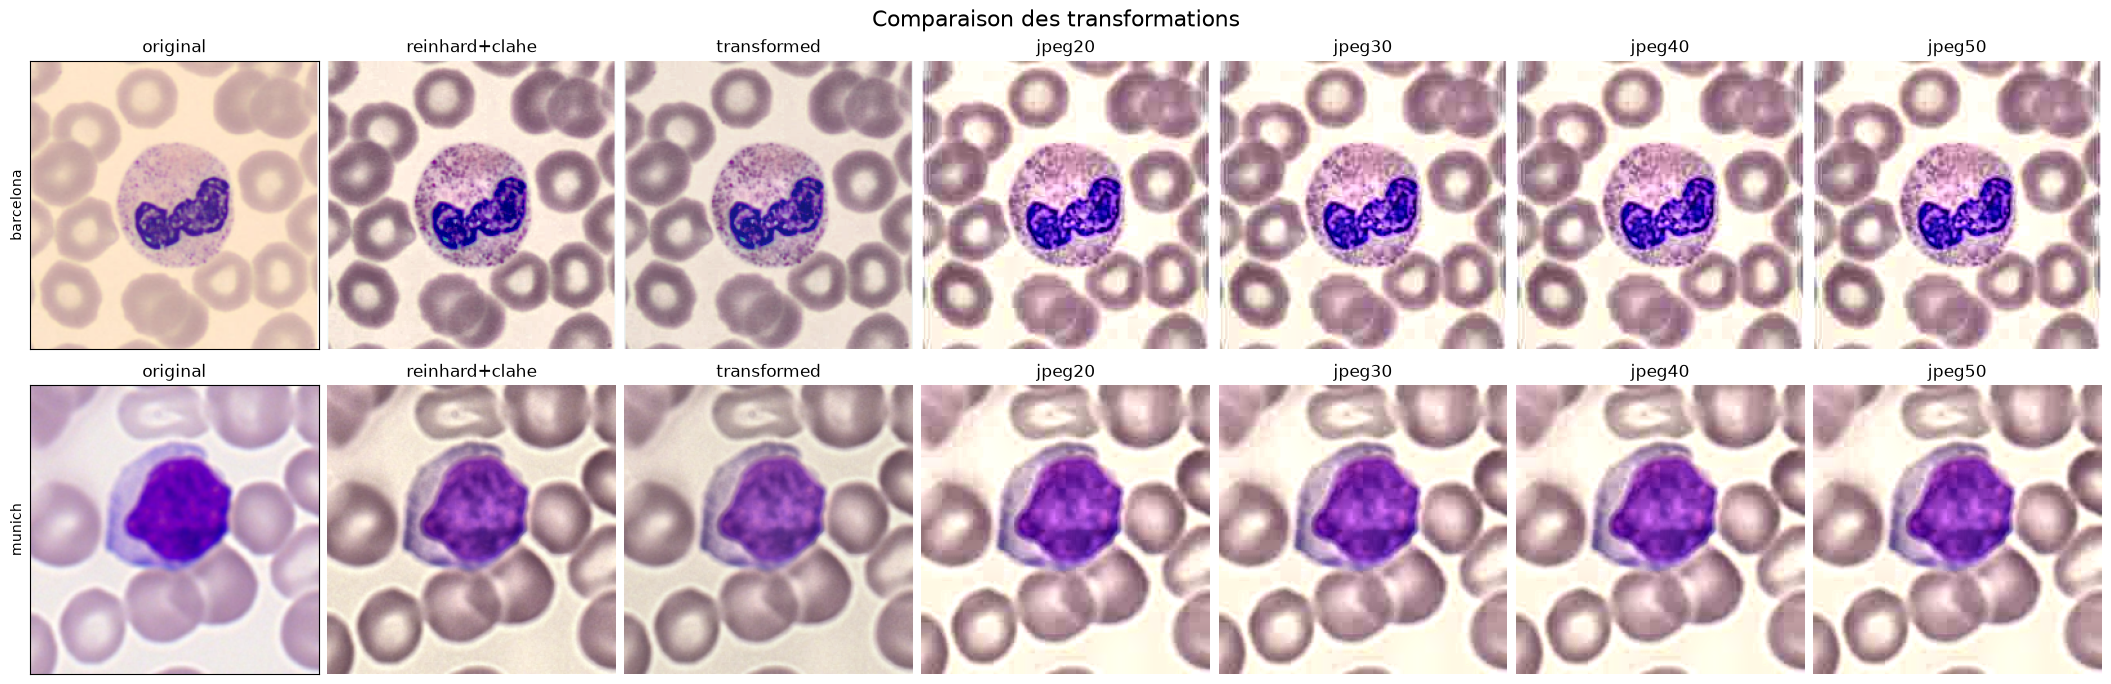
\includegraphics[width=\linewidth]{report/transforms_comparaison.png}
  \caption{Effet du pipeline sur une cellule de Barcelone (haut) et une de Munich (bas), étape par étape puis à différentes qualités JPEG.
Les fonds, initialement très différents, convergent vers un gris neutre.}
  \label{fig:transforms-comparaison}
\end{figure}

\paragraph{Méthodes écartées.} Une première approche recalait la moyenne et l’écart-type de \emph{chaque canal RGB} par dataset vers les statistiques globales : elle aligne bien les fonds mais reste trop grossière (elle n’agit ni sur la forme des distributions ni sur les interactions inter-canaux), et la PCA continue de séparer les sources.
La normalisation de \textbf{Macenko} \parencite{macenko2009normalizing} et celle de \textbf{Vahadane} \parencite{vahadane2016structurepreserving} ont également été testées puis écartées : conçues pour l’histologie H\&E, elles supposent \emph{deux} teintes dominantes, hypothèse fausse pour nos frottis May-Grünwald-Giemsa qui comptent bien plus de couleurs cliniquement significatives ; la décomposition devient instable et produit des dérives de couleur qui détruisent le signal porté par les granulations.
Leur sensibilité au choix de la référence et au type de coloration est un constat récurrent des comparaisons de méthodes \parencite{roy2018colornorm}.
Reinhard, purement statistique, ne fait aucune hypothèse sur le nombre de teintes.

\paragraph{Data augmentation (train uniquement).} Appliquée après l’harmonisation, sur le seul split d’entraînement, elle suit les recommandations usuelles pour l’imagerie \parencite{shorten2019survey}, en combinant transformations géométriques sûres et jitter photométrique modéré :

\begin{itemize}
  \item \textbf{géométrie} : rotation aléatoire de $\pm$180\textdegree{} (remplissage blanc), miroirs horizontal et vertical.
L’orientation d’une cellule sur la lame est arbitraire ; ces transformations n’altèrent pas les statistiques de couleur et servent aussi de rééquilibrage implicite des classes rares (plus de variantes vues par époque) ;
  \item \textbf{photométrie} : \texttt{ColorJitter} sur la luminosité ($\pm$0,15) et le contraste ($\pm$0,15), d’amplitude volontairement modérée : au-delà, la teinte des granulations sortirait de sa plage diagnostique.
Placé \emph{après} Reinhard : en amont, il serait annulé par le recalage vers des statistiques de couleur fixes.
Il rend le modèle robuste aux variations résiduelles de coloration et d’éclairage (variabilité inter-patients, vieillissement des lames) que l’harmonisation ne gomme pas entièrement.
\end{itemize}

\paragraph{Synthèse.} Le tableau~\ref{tab:transfo-synthese} récapitule les différences relevées entre les deux sources, le risque que chacune fait peser sur l’apprentissage et le traitement retenu.

\begingroup
\small
\setlength{\tabcolsep}{4pt}
\renewcommand{\arraystretch}{1.2}
\begin{longtable}{@{}>{\raggedright\arraybackslash}p{3.9cm} >{\raggedright\arraybackslash}p{5.1cm} >{\raggedright\arraybackslash}p{5.6cm}@{}}
  \caption{Différences entre sources, risque pour le modèle et traitement retenu.}\label{tab:transfo-synthese}\\
  \toprule
  \colhead{Différence observée} & \colhead{Risque pour le modèle} & \colhead{Traitement retenu} \\
  \midrule
  \endfirsthead
  \multicolumn{3}{@{}l}{\itshape\small Tableau~\ref{tab:transfo-synthese} (suite)}\\
  \toprule
  \colhead{Différence observée} & \colhead{Risque pour le modèle} & \colhead{Traitement retenu} \\
  \midrule
  \endhead
  \midrule
  \multicolumn{3}{r@{}}{\itshape\small suite page suivante}\\
  \endfoot
  \bottomrule
  \endlastfoot
  Résolution et ratio différents (360 $\times$ 363 contre 400 $\times$ 400 ; automates distincts) & Entrée non uniforme ; distorsion des cellules si redimensionnement naïf & \texttt{ResizeWithPad} 224 $\times$ 224, ratio préservé, \emph{padding} blanc \\
  Profondeur de canaux différente (RGB contre RGBA pour les TIFF de Munich) & Lecture incohérente : 4 canaux ou fond noir & \texttt{convert("RGB")} systématique à la lecture \\
  Format et compression (JPEG avec pertes contre TIFF sans perte ; poids $\times$40) & Artefacts de blocs 8 $\times$ 8 présents d’un seul côté $\rightarrow$ indice de site & Ré-encodage JPEG commun à tout le corpus (qualité 30) \\
  Teinte du fond (rose-beige chaud à Barcelone, gris-lilas froid à Munich) & Le modèle apprend le fond, c’est-à-dire le site, pas la cellule & Reinhard dans l’espace Lab, vers une cible neutre entre les deux sites \\
  Histogrammes RGB décalés entre sources & Séparabilité des sources (PCA) $\rightarrow$ raccourci d’apprentissage & Normalisation RGB globale (premier essai), puis Reinhard/Lab (retenu) \\
  Luminosité plus dispersée à Munich (200 patients, acquisition 2014--2017) & Sur-apprentissage des conditions d’éclairage ; fragilité en généralisation & Reinhard (canal L) et \texttt{ColorJitter} luminosité au train \\
  Contraste plus élevé et plus variable à Munich & Chromatine et granulations lues différemment selon le site & CLAHE sur le canal L et \texttt{ColorJitter} contraste au train \\
  Netteté plus faible sur une partie des images de Munich & Association « flou $\leftrightarrow$ site » ou « flou $\leftrightarrow$ classe mono-site » & CLAHE (rehausse le micro-contraste) ; contrôle qualité en amont pour les cas extrêmes \\
  Macenko inadapté (hypothèse de deux teintes, propre à l’histologie H\&E) & Dérives et inversions de couleur $\rightarrow$ perte du signal des granulations & Écarté au profit de Reinhard, sans hypothèse sur le nombre de teintes \\
  Classes rares et fort déséquilibre & Rappel effondré sur les classes minoritaires & Augmentation géométrique \\
  Orientation arbitraire des cellules (étalement manuel de la lame) & Sur-apprentissage d’orientations particulières & \texttt{RandomRotation} $\pm$180\textdegree{} et miroirs horizontal / vertical (train) \\
  Ordre des transformations (interaction jitter / Reinhard) & Le jitter colorimétrique serait annulé s’il précédait Reinhard & Jitter photométrique placé après Reinhard et CLAHE dans le \texttt{Compose} \\
\end{longtable}
\endgroup

\paragraph{Limites.} Les cibles de Reinhard et les statistiques de centrage-réduction sont figées à partir d’un sous-échantillon et devront être recalculées sur le split d’entraînement définitif.
Le \texttt{clip\_limit} de CLAHE, la qualité JPEG et l’amplitude du jitter sont des points de départ raisonnables, non optimisés.
Enfin, puisque l’harmonisation ne suffit pas à masquer la source à un CNN, les métriques des classes mono-site (plaquette, blaste) devront être lues avec une prudence particulière : un bon score sur ces classes peut refléter une reconnaissance du site autant que de la morphologie.

\section{Modélisation}
\label{sec:modelisation}

Le problème posé est, dans les deux cas, une \textbf{classification multi-classe} : soit sur les 10 types cellulaires fins retenus après fusion des deux jeux de données, soit sur les 3 niveaux de criticité clinique qui les regroupent (normal, intermédiaire, critique ; tableau~\ref{tab:fusion-taxonomie}).
Les deux tâches partagent la même architecture générale et le même pipeline d'entraînement ; elles ne diffèrent que par le nombre de classes en sortie et par le réglage de la fonction de perte associée (\S~\ref{sec:loss}).
Une variante binaire (normal contre anormal) est également dérivée de la criticité, pour la tâche métier de tri détaillée au \S~\ref{sub:metriques}.

Le projet a d'abord été développé avec Keras, puis migré vers PyTorch : l'écosystème PyTorch offre davantage de bibliothèques dédiées à la classification d'images et à l'accès à des modèles pré-entraînés (\emph{torchvision}, \texttt{timm}), une meilleure compatibilité entre versions, et de meilleures performances d'exécution sur les machines Mac utilisées par certains.

Pour explorer efficacement l'espace des choix de modélisation, un \textbf{framework d'expérimentation} maison a été développé.
Il permet de tester rapidement différents modèles (architectures maison ou \emph{backbones} pré-entraînés) ainsi que différentes configurations de transformation, d'augmentation et d'optimisation, sans dupliquer de code d'entraînement, tout en conservant une trace systématique des configurations utilisées et des résultats obtenus (recherche par grille, journal des runs).
C'est cette infrastructure qui permet notamment les comparaisons appariées multi-seed du \S~\ref{sec:grid-reequilibrage}.

Le travail de modélisation reprend la répartition présentée en introduction : \textbf{Romain} a développé ce framework d'expérimentation ainsi que la fonction de perte et les métriques adaptées, validés sur un modèle \emph{baseline} (\S~\ref{sec:baseline}) ; \textbf{Rémi} a exploré des architectures plus avancées et des approches par transfert (\S~\ref{sec:modele-avance}) ; \textbf{Joseph} a développé un modèle binaire par cellule (\S~\ref{sec:modele-binaire}) et un modèle hiérarchique.

\subsection{Optimisation}

Au-delà du choix de l’architecture, l’optimisation d’un modèle recouvre plusieurs décisions indépendantes : quelle \textbf{perte} minimiser (\S~\ref{sec:loss}), avec quel \textbf{optimiseur}, selon quel \textbf{calendrier de taux d’apprentissage}, et jusqu’à quand entraîner (\textbf{early stopping}).
Ces quatre aspects sont traités un à un dans cette sous-section.

\subsubsection{Loss}
\label{sec:loss}

Le jeu d’entraînement fusionné pose deux difficultés qu’une entropie croisée standard ne traite pas : il est \textbf{fortement déséquilibré} (rapport d’effectifs d’environ 17:1 entre le neutrophile et le promyélocyte pour la tâche fine à 10 classes, environ 7:1 entre paliers pour la tâche de criticité à 3 classes) et \textbf{cliniquement asymétrique} (rater un blaste est bien plus grave qu’une fausse alerte).
La perte utilisée dans le projet, \texttt{ClinicalLoss} (\texttt{src/models/losses.py}), combine trois leviers complémentaires, présentés un à un ci-dessous :

\begin{itemize}
  \item une \textbf{pondération par effectif}, qui rééquilibre la contribution de chaque classe à la perte selon sa rareté ;
  \item un \textbf{terme focal}, qui concentre l’apprentissage sur les exemples les plus ambigus, indépendamment de leur classe ;
  \item un \textbf{coût clinique}, qui pénalise plus fortement les confusions les plus graves plutôt que de traiter uniformément toutes les confusions d’une même classe.
\end{itemize}

Un quatrième levier, le \textbf{rééchantillonnage}, agit en amont sur les exemples présentés au modèle plutôt que sur la perte elle-même ; il est traité séparément au \S~\ref{sec:reechantillonnage}.
\texttt{ClinicalLoss} prend en entrée des logits bruts et des indices de classe entiers, comme \texttt{CrossEntropyLoss} ; \texttt{BCEWithLogitsLoss} reste utilisée telle quelle pour la tâche binaire de contrôle \texttt{dataset} (1 logit en sortie).

\paragraph{Pondération par effectif}
\label{sec:ponderation-effectif}

Il ne s'agit plus de compter chaque exemple à parts égales dans la perte, mais de donner plus de poids aux exemples des classes rares.
Sans correction, la perte moyenne est dominée par les classes majoritaires : le neutrophile ($\approx$ 12\,000 images) pèse près de 18 fois plus que le promyélocyte (680 images) dans le gradient moyen, alors que ce dernier est une classe critique.
Une pondération inverse-fréquence pure ($1/n_c$) corrigerait le déséquilibre, mais le surcorrige en général, au point d’écraser le signal des classes majoritaires.

Le poids $w_c$ d’une classe $c$ de $n_c$ exemples repose donc sur le \emph{nombre effectif d’échantillons} \parencite{cui2019classbalanced}, un compromis entre les deux extrêmes :
\[
  w'_c =
  \begin{cases}
    1 & \beta = 0 \quad \text{(pas de correction)} \\[4pt]
    \dfrac{1-\beta}{1-\beta^{\,n_c}} & 0 < \beta < 1 \quad \text{(nombre effectif)} \\[8pt]
    1/n_c & \beta = 1 \quad \text{(inverse-fréquence exacte)}
  \end{cases}
\]
$\beta \in [0,1]$ parcourt ainsi en continu l’absence de correction ($\beta=0$) jusqu’à l’inverse-fréquence pure ($\beta=1$).
Les valeurs usuelles pour $\beta$ sont supérieures à 0,99.

Un multiplicateur manuel optionnel \texttt{extra\_weight} (boost clinique, ex. $\times 1{,}5$ sur le blaste et le promyélocyte) peut s’ajouter à effectif égal ; les poids sont renormalisés pour que leur moyenne vaille 1 (ordre de grandeur de la perte stable).

À ce stade, la perte d’un exemple de classe vraie $y$ est une simple entropie croisée pondérée :
\[
  \mathcal{L}_i = -\, w_y \, \log p_y, \qquad p = \mathrm{softmax}(z).
\]

\paragraph{Terme focal}
\label{sec:terme-focal}

Au-delà du poids par classe, l’idée du terme focal est de moduler la contribution de \emph{chaque exemple} selon sa difficulté apparente, indépendamment de sa classe.
Même après pondération par effectif, la plupart des exemples d’une classe majoritaire sont rapidement bien classés (probabilité $p_y$ proche de 1) et continuent, par leur nombre, à dominer le gradient ; à l’inverse, les cas ambigus (ici la confusion morphologique attendue entre promyélocyte et blaste) restent sous-représentés dans le signal d’apprentissage malgré la seule pondération de classe.

Pour un exemple de classe vraie $y$ et $p_y$ sa probabilité prédite, le facteur focal \parencite{lin2017focal}
\[
  (1 - p_y)^{\gamma}, \qquad \gamma = 0 \Rightarrow \text{désactivé},
\]
éteint progressivement la contribution des exemples déjà bien classés ($p_y \to 1$) et concentre le gradient sur les exemples ambigus ou mal classés.

En ajoutant ce terme à la pondération par effectif, la perte devient :
\[
  \mathcal{L}_i = -\, w_y \,(1 - p_y)^{\gamma} \, \log p_y .
\]

\paragraph{Coût clinique}
\label{sec:cout-clinique}
Ce levier ne pondère plus seulement selon la classe vraie : il encode directement le coût de chaque \emph{type de confusion}.
Une pondération de classe, même précise, sur-pondère le rappel d’une classe rare globalement, mais ne distingue pas « critique confondu avec normal » (raté grave) de « critique confondu avec intermédiaire » (moins grave), deux erreurs pourtant très différentes en pratique clinique.

On encode donc ce coût dans une matrice $M \in \mathbb{R}^{K \times K}$, où $M_{i,j}$ est le coût de prédire la classe $j$ quand la vraie classe est $i$ (diagonale nulle), l’approche classique de l’apprentissage sensible au coût \parencite{elkan2001costsensitive,kukar1998costsensitive}.
Les matrices utilisées par défaut, dans l’espace de la \textbf{criticité} (normal / intermédiaire / critique, ou normal / anormal en binaire) :
\[
  M_3 = \begin{pmatrix} 0 & 0{,}5 & 1 \\ 4 & 0 & 1 \\ 10 & 3 & 0 \end{pmatrix},
  \qquad
  M_2 = \begin{pmatrix} 0 & 1 \\ 10 & 0 \end{pmatrix}.
\]
La ligne « critique » de $M_3$ rend une confusion critique~$\to$~normal dix fois plus coûteuse qu’une fausse alerte normal~$\to$~critique : le principe « faux négatif $\gg$ faux positif » est traduit au niveau de chaque paire (classe vraie, classe prédite), pas seulement de la classe vraie.

Pour la tâche fine à \textbf{10 classes}, une matrice $2\times2$ ou $3\times3$ n’a pas directement la bonne dimension : elle est alors \emph{liftée} en reportant le coût du palier de criticité de chaque classe, $M_{10}[i,j] = M_{3}[\,\mathrm{crit}(c_i),\,\mathrm{crit}(c_j)\,]$, où $\mathrm{crit}(\cdot)$ est le palier de la classe (\texttt{src/constants.py::CRITICALITY}).
Conséquence directe : le coût est \textbf{nul} entre deux classes du même palier (par exemple blaste $\leftrightarrow$ promyélocyte, toutes deux critiques) et maximal pour confondre une classe critique avec une classe normale : c’est alors le terme d’entropie croisée qui porte seul la discrimination \emph{fine} à l’intérieur d’un même palier.
Une matrice déjà fournie à la dimension de la tâche est utilisée telle quelle.

Le coût espéré, différentiable,
\[
  \mathrm{EC}_i = \sum_{c=1}^{K} M_{y_i,\,c}\; p_c ,
\]
pénalise le modèle dès qu’il place de la masse de probabilité sur une classe coûteuse, avant même que sa prédiction finale (\emph{argmax}) ne se trompe.
Pondéré par $\lambda$ (\texttt{lambda\_cost}, 0 = désactivé) et ajouté aux termes de \hyperref[sec:ponderation-effectif]{pondération par effectif} et \hyperref[sec:terme-focal]{focal}, il donne la perte complète :
\[
  \mathcal{L}_i \;=\; \underbrace{-\, w_y\,(1-p_y)^{\gamma}\,\log p_y}_{\text{pondération + focale}} \;+\; \underbrace{\lambda \sum_{c} M_{y_i,\,c}\; p_c}_{\text{coût espéré}} .
\]

\paragraph{Limites}
\label{sec:limites-loss}

Une matrice de coût, comme tout hyperparamètre porteur d’une hypothèse forte, doit être calibrée sur le jeu de données réel : une valeur par défaut raisonnable \emph{a priori} peut être largement sur-dimensionnée pour un déséquilibre particulier.
Les valeurs retenues ici sont spécifiques à cette taxonomie et à ce déséquilibre.
Plus généralement, une perte pondérée ou sensible au coût déplace le compromis précision / rappel \emph{en espérance} pendant l’entraînement, mais le niveau de rappel réellement atteint doit toujours être vérifié par classe sur des données non vues (validation puis test).
Un ajustement du seuil de décision en post-traitement reste souvent nécessaire pour une cible de rappel précise sur les classes critiques.
Enfin, toute comparaison entre configurations dont l’écart est inférieur à la variance inter-seed observée sur les classes rares (jusqu’à 0,18 de rappel critique entre seeds pour une même configuration sur \texttt{type}) n’est pas interprétable sans réplication multi-seed appariée.

\subsubsection{Rééchantillonnage (\emph{weighted random sampler})}
\label{sec:reechantillonnage}

Le déséquilibre peut aussi être corrigé en amont, du côté de l’\textbf{échantillonnage}. 
Avec \texttt{train.sampler = weight}, le \texttt{DataLoader} d’entraînement utilise un \texttt{WeightedRandomSampler} : à chaque époque, les exemples sont tirés \emph{avec remise} (autant que la taille du split) proportionnellement à un poids de classe
\[
  \pi_c \;\propto\; \left(\frac{1}{n_c}\right)^{\!\alpha},
\]
normalisé pour que la moyenne des poids de classe vaille 1 (même convention que les poids de la perte). 
L’exposant $\alpha$ (\texttt{sampler\_alpha}) règle l’intensité : $\alpha = 0$ redonne un tirage uniforme (le sampler n’a aucun effet), $\alpha = 1$ correspond à l’inverse-fréquence pleine (toutes les classes deviennent équiprobables en espérance), $\alpha = 0{,}5$ à un compromis « racine ». 
La figure~\ref{fig:sampler-alpha} montre l’effectif attendu par classe et par époque pour quelques valeurs de $\alpha$.

\begin{figure}[ht]
  \centering
  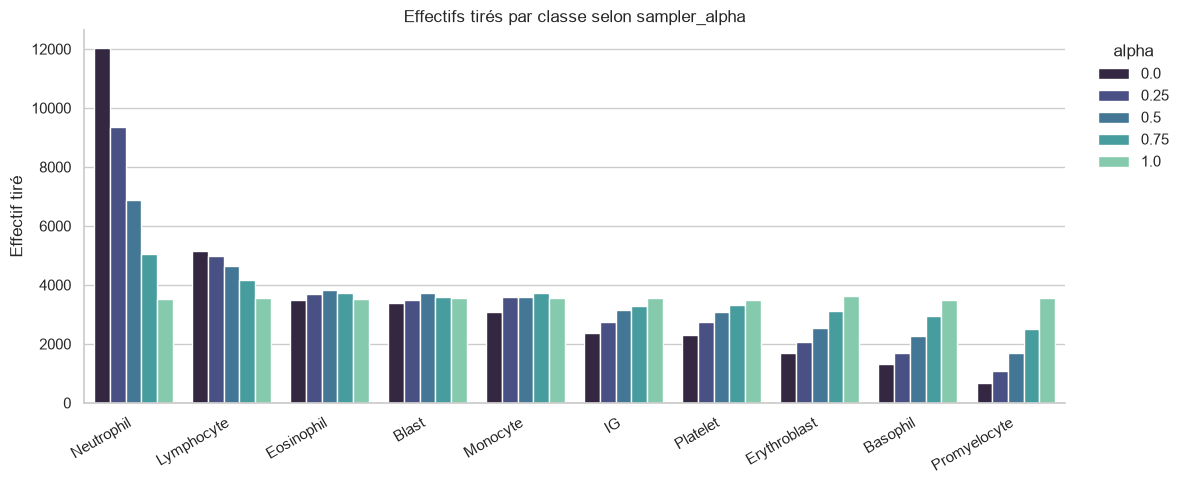
\includegraphics[width=0.92\linewidth]{report/sampler_alpha.png}
  \caption{Effectif tiré par classe et par époque selon \texttt{sampler\_alpha}.
À $\alpha = 0$, la distribution suit le déséquilibre brut ($\approx$ 12\,000 neutrophiles contre 680 promyélocytes) ; à $\alpha = 1$, toutes les classes convergent vers le même effectif ; les valeurs intermédiaires interpolent entre les deux.}
  \label{fig:sampler-alpha}
\end{figure}

En matérialisant les indices tirés pour chaque valeur de $\alpha$, on chiffre l'effet sur deux indicateurs synthétiques : le rapport d'effectifs maximum / minimum et l'entropie de Shannon normalisée du tirage (1 = équilibre parfait). 
Sur la nomenclature à 10 classes (tableau~\ref{tab:sampler-alpha}), le déséquilibre brut se résorbe régulièrement, l'entropie franchissant 0,97 dès $\alpha = 0{,}5$. 
Le prix est une \textbf{redondance croissante des classes rares} : à $\alpha = 1$, les 680 images de promyélocyte donnent lieu à $\approx$ 3\,550 tirages, soit chaque image vue environ \textbf{cinq fois par époque}, tandis que chaque neutrophile n'est vu qu'une fois sur trois. 
C'est l'argument principal pour ne pas pousser $\alpha$ jusqu'à 1 et pour coupler le sampler à l'augmentation.

\begin{table}[H]
  \centering
  \small
  \renewcommand{\arraystretch}{1.15}
  \begin{tabular}{@{}cccc@{}}
    \toprule
    $\alpha$ & Rapport max/min & Entropie normalisée & Neutrophiles / promyélocytes tirés \\
    \midrule
    0{,}00 & 17{,}5 & 0{,}87 & 12\,000 / 670 \\
    0{,}25 & 8{,}8  & 0{,}93 & 9\,350 / 1\,070 \\
    0{,}50 & 4{,}1  & 0{,}97 & 6\,900 / 1\,700 \\
    0{,}75 & 2{,}0  & 0{,}99 & 5\,030 / 2\,510 \\
    1{,}00 & 1{,}0  & 1{,}00 & 3\,530 / 3\,550 \\
    \bottomrule
  \end{tabular}
  \caption{Effet de \texttt{sampler\_alpha} sur le déséquilibre du tirage (10 classes).
Le déséquilibre brut du jeu de données correspond à $\alpha = 0$ (rapport 17,5).}
  \label{tab:sampler-alpha}
\end{table}

\paragraph{Couplage avec la pondération de la perte.} 
Le sampler et les poids de la perte agissent sur le \emph{même} déséquilibre : les appliquer tous les deux à pleine intensité le corrige \emph{deux fois} et pousse le modèle à sur-représenter les classes rares. 
On répartit donc la correction : sampler seul, perte pondérée seule, ou un sampler partiel ($\alpha \approx 0{,}5$) complété par la pondération de la perte (\texttt{loss.beta} modéré, sans double comptage).
Découpler ainsi l’apprentissage de la représentation (tirage proche des fréquences réelles) de celui du classifieur (rééquilibré) est une recette éprouvée en reconnaissance \emph{long-tail} \parencite{kang2020decoupling}. 

Les deux leviers ne sont pas équivalents : le sampler équilibre les gradients \emph{à l’échelle du mini-batch} (utile à la stabilité de la \emph{batch normalization} et à la convergence des classes rares), mais réutilise beaucoup les mêmes images rares par époque (jusqu’à cinq fois pour le promyélocyte, cf.\ tableau~\ref{tab:sampler-alpha}) ; d’où l’intérêt de l’augmentation géométrique, qui en diversifie les variantes.
La pondération de la perte ne duplique aucune image mais produit des gradients plus bruités sur les classes rares, peu représentées dans chaque batch.

\subsubsection{Grid search sur le rééquilibrage}
\label{sec:grid-reequilibrage}

\paragraph{Une matrice par défaut mal calibrée peut sembler inutile.}
Le premier essai du terme de coût sur la tâche \texttt{criticality}, avec la matrice $M_3$ par défaut (\hyperref[sec:cout-clinique]{coût clinique}), dégradait le F1 macro (jusqu’à 0,88, contre 0,919 pour \emph{class-balanced} + focale seules) sans le moindre gain de rappel critique.
La première réaction a été de penser que ce terme était inutile pour ce projet.
En réalité, ses coûts d'erreurs vers la criticité normal (10 et 4) étaient trop élevés pour ce déséquilibre précis : le modèle sur-prédisait les paliers supérieurs pour éviter la pénalité, perdant en précision sans gagner de rappel. 
Une fois la matrice ajustée (abaisser critique$\to$normal de 10 à 4, intermédiaire$\to$normal de 4 à 2), le terme de coût devient au contraire le meilleur levier de la tâche. 

Il a alors été décidé de réaliser une \textit{grid search} pour explorer l'ensemble des paramètres associés à la fonction de perte et au rééchantillonage.
Cette recherche a été effectuée aussi bien sur la tâche avec 3 classes de criticité que sur la tâche avec les 10 types de cellule.
On a donc balayé l'espace des paramètres pour $\beta\in[0, 0.99, 0.999, 0.9999, 1]$, $\gamma\in[0, 0.5, 1, 2]$, $\alpha\in [0, 0.5, 1]$ et pour différentes matrices de coût clinique.
Afin de limiter l'effet aléatoire, on a utilisé plusieurs seeds aléatoires identiques pour chaque configuration.
On a ensuite comparé la moyenne et l'écart type du $f1$-score et du rappel critique minimal, c'est-à-dire le plus faible rappel parmi les classes critiques.

\paragraph{Les deux tâches n’ont pas le même optimum.}
Le tableau~\ref{tab:imbalance-grid} compare, pour chacune des tâches \texttt{criticality} (3 paliers) et \texttt{type} (10 classes), la meilleure combinaison \emph{sans} matrice de coût à la configuration retenue \emph{avec}.

\begin{table}[H]
  \centering
  \small
  \renewcommand{\arraystretch}{1.25}
  \begin{tabularx}{\textwidth}{@{}l X cc@{}}
    \toprule
    Tâche & Configuration (validation, multi-seed) & F1 macro & Rappel critique min. \\
    \midrule
    Criticité (3) & \emph{Class-balanced} + focale, sans coût ($\beta{=}0{,}9999,\gamma{\approx}2$) & 0,919 & 0,957 \\
    Criticité (3) & \textbf{Retenue} : coût calibré seul ($\lambda{=}1$, $\beta{=}\gamma{=}0$) & 0,909 & \textbf{0,964} \\
    Type (10)     & \emph{Class-balanced} + focale + sampler, sans coût & 0,867 & 0,845 \\
    Type (10)     & \textbf{Retenue} : coût calibré + sampler plein ($\alpha{=}1$) + $\beta{=}0{,}999$ & 0,871 & \textbf{0,910} \\
    \bottomrule
  \end{tabularx}
  \caption{Comparaison des stratégies de rééquilibrage sur la validation, moyenne multi-seed appariée (47 configurations $\times$ 3 seeds).
Le « rappel critique minimal » est le plus faible rappel parmi les classes/paliers critiques.}
  \label{tab:imbalance-grid}
\end{table}

Sur \texttt{criticality}, le coût calibré \textbf{seul} dépasse déjà \emph{class-balanced} + focale sur le critère qui compte (rappel critique), et ajouter sampler ou pondération par-dessus n’apporte \textbf{aucun gain net} une fois la matrice active : $\beta$ y devient redondant.
Sur \texttt{type}, à l’inverse, \textbf{cumuler les trois leviers aide} : le déséquilibre y est trop sévère (17,5 contre $\approx$ 6,9) pour qu’un rééchantillonnage partiel ou une matrice seule suffisent ; il faut le sampler à pleine intensité \emph{et} une pondération de classe non nulle \emph{et} la matrice de coût.
La recette qui gagne sur une tâche n’est donc pas transposable telle quelle à l’autre : le degré de rééquilibrage nécessaire dépend de la sévérité du déséquilibre, pas seulement de la présence de classes critiques.

\subsubsection{Optimizer}
\label{sec:optimizer}

Trois optimiseurs sont disponibles (\texttt{optim.name}, construits par \texttt{build\_optimizer} dans \texttt{src/training/components.py}), sans qu’il soit nécessaire de revenir sur leur formulation mathématique pour justifier le choix retenu.

\begin{itemize}
  \item \textbf{SGD} \parencite{bottou2010sgd} (descente de gradient stochastique, avec un unique taux d’apprentissage global) : la recette historique, encore utilisée dans des architectures comme ResNet, mais qui demande un réglage plus fin du taux d’apprentissage et un bon calendrier pour converger aussi bien qu’une méthode adaptative.
  \item \textbf{Adam} \parencite{kingma2015adam} : adapte un pas par paramètre à partir des moments (moyenne, variance) du gradient, ce qui le rend nettement moins sensible au réglage du taux d’apprentissage et généralement plus rapide à converger : c’est l’optimiseur utilisé par défaut dans le projet.
  \item \textbf{AdamW} \parencite{loshchilov2019decoupled} : variante d’Adam qui découple la régularisation \emph{weight decay} de la mise à jour adaptative, corrigeant un couplage indésirable présent dans l’Adam original dès que \texttt{weight\_decay} > 0.
\end{itemize}

Quelques tests de comparaison directe (mêmes hyperparamètres de perte et de scheduler, seul \texttt{optim.name} change) n’ont montré aucun intérêt à s’écarter d’Adam sur ce projet.
Sur la tâche \texttt{type}, le run final rejoué avec AdamW obtient un F1 macro test de 0,911 contre 0,916 pour Adam : la correction apportée par AdamW n’a ici aucun effet mesurable.
SGD n’a pas été creusé davantage : sur les budgets d’entraînement courts utilisés pendant le \emph{grid search} (quelques époques par configuration), l’absence de taux adaptatif se traduirait par un coût de réglage supplémentaire (taux d’apprentissage, momentum, calendrier) pour un gain non démontré.
Adam reste donc l’optimiseur utilisé pour l’ensemble des expériences du rapport.

\subsubsection{Learning rate scheduler}

Un taux d’apprentissage fixe est un compromis qui n’est bon qu’à un instant de l’entraînement : trop grand, les mises à jour oscillent autour d’un minimum sans s’y stabiliser ; trop petit, la convergence est lente et gaspille le budget de calcul.
Un \emph{scheduler} fait décroître le taux d’apprentissage au cours de l’entraînement selon une règle définie, typiquement pour autoriser un grand pas au début (exploration) et un petit pas à la fin (convergence fine).
Adam atténue la sensibilité au réglage du taux d’apprentissage (\S~\ref{sec:optimizer} ci-dessus) mais ne réduit pas de lui-même le pas \emph{global} en fin d’entraînement : un scheduler reste donc utile même avec un optimiseur adaptatif.

Le scheduler est construit par \texttt{build\_scheduler} (\texttt{src/training/components.py}) à partir de \texttt{scheduler.name}, puis appelé une fois par époque dans la boucle d’entraînement (\texttt{Trainer.fit}), après l’étape d’optimisation \parencite{pytorchoptim}.
Trois politiques non triviales sont implémentées, plus une référence sans décroissance :

\begin{itemize}
  \item \texttt{none} : taux constant, référence de comparaison.
  \item \texttt{plateau} (\texttt{ReduceLROnPlateau}) : réduit le taux d’un facteur fixe dès que la \texttt{val\_loss} cesse de s’améliorer pendant \texttt{scheduler.patience} époques consécutives. Piloté par les données plutôt que par un calendrier arbitraire, ce qui le rend robuste sans connaissance préalable du nombre d’époques nécessaires, au prix d’une réaction \emph{après coup} et d’une sensibilité au bruit de la \texttt{val\_loss} sur les classes rares.
  \item \texttt{cosine} (\texttt{CosineAnnealingLR}, \parencite{loshchilov2017sgdr}) : décroissance lisse en demi-période de cosinus jusqu’à \texttt{scheduler.lr\_min}, sur un horizon fixé à \texttt{train.nb\_epoch}. Ne demande quasiment aucun réglage, mais exige de connaître le nombre d’époques à l’avance et se combine mal à un early stopping serré, qui couperait le calendrier avant sa fin.
  \item \texttt{step} (\texttt{StepLR}) : divise le taux par \texttt{scheduler.step\_gamma} tous les \texttt{train.nb\_epoch}~/~3 époques. Simple et reproductible, mais introduit des chutes brutales et dépend, comme \texttt{cosine}, du nombre total d’époques.
\end{itemize}

En pratique, le \emph{grid search} de rééquilibrage (\S~\ref{sec:grid-reequilibrage}) s’est appuyé sur des budgets courts et fixes (3 à 10 époques par configuration), pour lesquels un scheduler apporte peu ; \texttt{plateau} a ensuite été retenu pour les runs finaux (\texttt{scheduler.patience = 3}), \texttt{cosine} et \texttt{step} n’ayant pas été exercés faute d’un budget d’époques fixé à l’avance qui en justifierait l’usage.

\subsubsection{Early stopping}

Fixer le nombre d’époques à l’avance pose un problème symétrique de celui du taux d’apprentissage : trop peu sous-entraîne le modèle, trop remonte la \texttt{val\_loss} par surapprentissage alors que la perte d’entraînement continue de baisser.
Le nombre optimal d’époques dépend du modèle, des données, de la perte et du \emph{sampler} : il n’est pas connu à l’avance et change à chaque configuration du \emph{grid search}, ce qui rend impraticable de le fixer manuellement pour chacune.
L’\textbf{early stopping} \parencite{prechelt1998earlystopping,goodfellow2016deeplearning} (\texttt{EarlyStopping}, \texttt{src/training/callbacks.py}) résout ce problème en arrêtant l’entraînement dès que la métrique surveillée cesse de progresser, et en restaurant les poids de la meilleure époque plutôt que ceux de la dernière.

À chaque fin d’époque, \texttt{Trainer.fit} appelle \texttt{step(epoch\_metrics, model)} sur chaque callback actif, qui compare \texttt{val\_loss} à sa meilleure valeur observée.
Si aucune amélioration n’est observée pendant \texttt{train.early\_\allowbreak stopping\_\allowbreak patience} époques consécutives, l’entraînement s’interrompt et \texttt{restore()} recharge le \texttt{state\_dict} de la meilleure époque, copié à chaque amélioration.

L’early stopping et le scheduler \texttt{plateau} s’appuient sur le même signal (\texttt{val\_loss}) mais avec des objectifs différents : le scheduler \emph{réagit} à la stagnation en réduisant le taux d’apprentissage, l’early stopping en \emph{conclut} qu’il faut arrêter.
Si l’arrêt intervient avant que la réduction du taux n’ait eu le temps de produire son effet, le scheduler ne sert à rien ; la configuration retenue pour les runs finaux (\texttt{scheduler.patience = 3}, \texttt{train.early\_stopping\_patience = 10}) laisse ainsi une marge d’environ trois réductions de palier avant l’arrêt définitif.
Sur les budgets courts et fixes du \emph{grid search} lui-même (3 à 10 époques), cette patience de 10 dépassait souvent le budget total et l’early stopping n’y jouait donc quasiment aucun rôle ; il n’a été réellement actif que pour les runs finaux (\texttt{nb\_epoch = 50}), où il a permis de fixer une borne haute généreuse sans avoir à deviner le bon nombre d’époques pour chaque tâche.

\subsection{Métriques}
\label{sub:metriques}

Le choix des métriques est dicté par les deux mêmes contraintes que la perte : un \textbf{déséquilibre fort} (17:1 entre neutrophile et promyélocyte) et une \textbf{asymétrie clinique} (un faux négatif sur une classe critique coûte bien plus qu'une fausse alerte).
L'\emph{accuracy} globale est donc écartée comme métrique de pilotage : à 34\,\% de neutrophiles, un modèle qui ne prédirait que la classe majoritaire afficherait déjà une accuracy trompeusement élevée tout en manquant l'intégralité des blastes.
Les métriques sont implémentées dans \texttt{src/models/metrics.py} au-dessus de \texttt{torchmetrics} ; \texttt{build\_metrics()} renvoie une collection légère (accuracy, F1 micro) pour le \emph{logging} par epoch et une collection complète, détaillée au tableau~\ref{tab:metriques}, pour l'évaluation finale sur le test.

\paragraph{Vue d'ensemble : F1 macro et MCC.} Le \textbf{F1 macro} (moyenne non pondérée des F1 par classe) donne à chaque classe le même poids quel que soit son effectif : il chute dès qu'une classe rare est mal traitée, ce que le F1 micro masquerait.
Il sert de critère d'optimisation secondaire lors de la sélection de modèle.
Le \textbf{coefficient de corrélation de Matthews} (MCC) le complète : calculé à partir de l'ensemble de la matrice de confusion, il n'est élevé que si le modèle réussit simultanément sur toutes les classes, et reste fiable en contexte déséquilibré là où l'accuracy et le F1 peuvent être gonflés \parencite{chicco2020mcc,grandini2020metrics}.
C'est la métrique de résumé rapportée en priorité pour comparer deux modèles d'un coup d'\oe{}il.

\paragraph{Analyse par classe : rappel, précision et $F_\beta$.} Une moyenne, même macro, masque \emph{quelle} classe pose problème.
On rapporte donc le \textbf{rappel} et la \textbf{précision} par classe (\texttt{average=None}).
Le rappel des classes \textbf{critiques} et \textbf{intermédiaires} (tableau~\ref{tab:fusion-taxonomie}) est la grandeur décisive : c'est la proportion de blastes, promyélocytes, granulocytes immatures et érythroblastes effectivement détectés.
On y adjoint le \textbf{$F_\beta$ avec $\beta = 2$}, qui pondère le rappel quatre fois plus que la précision ($\beta^2$) et traduit numériquement la préférence « mieux vaut une fausse alerte qu'un raté » sur ces classes ; il n'est lu que sur les indices critiques et modérés, pour lesquels ce compromis est justifié.

\paragraph{Métriques indépendantes du seuil : AUPRC.} Le rappel, la précision et le $F_\beta$ dépendent du seuil de décision (\emph{argmax} par défaut), or ce seuil sera réajusté en post-traitement pour atteindre la cible de rappel critique (cf.\ \hyperref[sec:limites-loss]{limites de la perte}).
Pour évaluer la qualité intrinsèque du classifieur indépendamment de ce réglage, on calcule l'\textbf{AUPRC} (aire sous la courbe précision-rappel, \emph{average precision}) par classe, en un-contre-tous, à partir des probabilités \emph{softmax}.
La courbe précision-rappel est préférée à la courbe ROC : en fort déséquilibre, la ROC-AUC est optimiste car les vrais négatifs, très nombreux, dominent le taux de faux positifs et masquent les erreurs sur la classe rare \parencite{saito2015prc}.
L'AUPRC d'une classe rare, elle, s'effondre dès que les faux positifs deviennent comparables en nombre aux quelques positifs réels.

\paragraph{Matrice de confusion et direction dangereuse.} La matrice de confusion complète ($10 \times 10$) est inspectée sous deux formes : comptes bruts et version normalisée par ligne (dont la diagonale est le rappel).
Au-delà de l'inspection visuelle, on extrait automatiquement (\texttt{critical\_\allowbreak to\_\allowbreak normal\_\allowbreak confusion()}) la sous-matrice des confusions \textbf{« classe anormale vraie $\rightarrow$ classe mature normale prédite »} : c'est la seule direction d'erreur cliniquement grave (un blaste vu comme un lymphocyte), à distinguer d'une confusion entre deux classes anormales, bien moins préoccupante.
Le nombre absolu d'erreurs dans cette sous-matrice est un indicateur de sûreté rapporté explicitement.

\paragraph{Rappel critique minimum.} Le \textbf{rappel critique minimum} (\texttt{min\_critical\_recall}) est le minimum du rappel par classe restreint aux classes critiques (blaste, promyélocyte) : il désigne la classe critique la plus fragile d'un run, là où une moyenne pourrait masquer une classe rare mal détectée.
C'est la valeur rapportée dans les tableaux de résultats sous l'intitulé « rappel critique, min. classe » ; dans la quasi-totalité des expériences de ce rapport, c'est le promyélocyte, la classe la plus rare, qui l'atteint.

\paragraph{Rappel critique groupé et screening.} Sur la tâche \texttt{type}, deux métriques dérivées du \textbf{groupe critique} (blaste + promyélocyte) complètent le rappel par classe.
Le \textbf{rappel critique groupé} (\texttt{grouped\_critical\_recall}) répond à la question opérationnelle réelle : parmi les cellules vraiment critiques, quelle proportion est prédite dans le groupe critique, \emph{quel que soit le type exact} ?
Confondre blaste et promyélocyte y est neutre ; ne prédire ni l'un ni l'autre pour une cellule réellement critique fait manquer la revue.
Il est donc structurellement $\geq$ au rappel critique minimum décrit ci-dessus et s'en distingue par nature : le premier mesure si le \emph{tri} fonctionne, le second si chaque \emph{type} critique est correctement reconnu.

L'\textbf{AP de criticité} (\texttt{critical\_screening\_ap}) résume, indépendamment du seuil, un second score dérivé : la masse de probabilité \emph{softmax} sur le groupe critique ($P(\text{blaste}) + P(\text{promyélocyte})$), comparée au label binaire « la cellule est-elle critique ? ».
C'est l'\emph{average precision} de ce score, selon la même logique que l'AUPRC par classe ci-dessus, appliquée cette fois au groupe critique amalgamé plutôt qu'à une classe individuelle.
Elle alimente la courbe de \textbf{screening critique} (\texttt{critical\_screening\_prc}, figure~\ref{fig:baseline-critical-screening}) : en abaissant le seuil de décision sous l'\emph{argmax} par défaut, on trace le rappel critique atteignable en fonction de la \emph{charge de revue} (part des images envoyées en relecture), l'ajustement de seuil déjà anticipé au \hyperref[sec:limites-loss]{limites de la perte}.
\texttt{screening\_operating\_points()} en extrait deux points de fonctionnement (seuil, précision, charge de revue) aux cibles de rappel 0,95 et 0,99.

\paragraph{Rappel top-3.} Sur les tâches à $\geq 5$ classes, on rapporte également l'\textbf{accuracy top-3} (micro) et le \textbf{F1 macro top-3} : la vraie classe figure-t-elle parmi les 3 scores les plus élevés ?
Une valeur élevée malgré un F1 macro modeste indique un modèle qui hésite entre des classes morphologiquement voisines plutôt que franchement dans l'erreur : une nuance utile pour un outil d'aide à la décision qui proposerait plusieurs classes candidates plutôt qu'une seule.

\paragraph{Métrique de la tâche métier « normal contre anormal ».} Le deuxième objectif du projet est un détecteur binaire d'anomalie.
Indépendamment de la tâche fine à 10 classes, on collapse les prédictions et les labels en \texttt{normal} / \texttt{anormal} (\texttt{to\_binary\_abnormal()}, les classes critiques et intermédiaires devenant « anormal ») et on rapporte \textbf{rappel, précision et F1 binaires}.
Cela mesure directement la capacité à trier les lames nécessitant une relecture humaine, sans exiger que le type cellulaire exact soit correct.

\begin{table}[H]
  \centering
  \small
  \setlength{\tabcolsep}{5pt}
  \renewcommand{\arraystretch}{1.2}
  \begin{tabular}{@{}>{\raggedright\arraybackslash}p{3.1cm} >{\raggedright\arraybackslash}p{4.0cm} >{\raggedright\arraybackslash}p{6.2cm}@{}}
    \toprule
    \textbf{Métrique} & \textbf{Portée} & \textbf{Pourquoi} \\
    \midrule
    F1 macro            & globale, par classe équipondérée & insensible au déséquilibre ; critère secondaire de sélection \\
    MCC                 & globale, matrice entière         & résumé fiable en contexte déséquilibré \parencite{chicco2020mcc} \\
    Rappel par classe   & chaque classe                    & proportion de cellules critiques réellement détectées \\
    Précision par classe & chaque classe                   & contrôle du volume de fausses alertes \\
    Rappel critique min.\ & min sur les classes critiques & identifie la classe critique la plus fragile d'un run \\
    $F_\beta$, $\beta=2$ & classes critiques / intermédiaires & pondère le rappel $\times 4$ : « rater $\gg$ fausse alerte » \\
    AUPRC (AP)          & chaque classe, un-contre-tous     & qualité indépendante du seuil ; adaptée aux classes rares \parencite{saito2015prc} \\
    Matrice de confusion & 10 classes + sous-matrice anormal$\rightarrow$normal & localise les confusions ; isole la direction dangereuse \\
    Rappel critique groupé & groupe critique (blaste + promyélocyte), \emph{argmax} & la cellule critique est-elle envoyée en revue, quel que soit son type exact \\
    AP de criticité (screening) & groupe critique, indépendant du seuil & qualité du tri critique/normal ; alimente la courbe de screening (rappel vs charge de revue) \\
    Top-3 accuracy / F1 & globale (tâches $\geq 5$ classes) & tolère l'hésitation entre classes voisines, utile en aide à la décision \\
    Rappel / préc.\ / F1 binaires & tâche normal vs anormal    & mesure directe du tri pour relecture humaine \\
    \bottomrule
  \end{tabular}
  \caption{Métriques d'évaluation retenues et justification.
  Les moyennes globales servent à comparer des modèles ; les métriques par classe et la matrice de confusion servent à vérifier que le compromis clinique est tenu.}
  \label{tab:metriques}
\end{table}

\subsection{Modèles}
\subsubsection{Modèlisation binaire par cellule}
\label{sec:modele-binaire}
Une première baseline de classification binaire a été mise en place afin d’évaluer la capacité des données à discriminer un type cellulaire de l’ensemble des autres classes.
Cette approche consiste à considérer successivement une classe comme classe positive et toutes les autres comme classe négative.

Cette stratégie permet d’obtenir une première évaluation de la \textbf{séparabilité des différentes populations cellulaires} et de comparer les difficultés rencontrées selon les classes.
Elle permet également de mettre en évidence d’éventuels problèmes présents dans les données, notamment lorsque certaines erreurs de classification peuvent être associées à des images ambiguës.

Les premières expérimentations ont notamment porté sur les \textbf{neutrophiles segmentés} puis sur les \textbf{promyélocytes}.
Le choix d’une approche binaire permet de se concentrer sur une population cellulaire donnée et d’observer plus précisément sa capacité à être distinguée du reste du jeu de données.

Cette baseline constitue également un premier moyen de vérifier si les caractéristiques présentes dans les images sont suffisamment discriminantes pour permettre une classification.
Les résultats obtenus doivent cependant être interprétés avec prudence : une bonne performance de classification ne garantit pas que le modèle s’appuie sur les caractéristiques morphologiques pertinentes de la cellule.
En particulier, compte tenu des différences observées entre les sources PBC et LMU, le modèle peut potentiellement exploiter des caractéristiques liées au \textbf{site d’acquisition} plutôt qu’à la cellule elle-même.

Ces travaux de modélisation, menés en complément de l’exploration des données, apportent ainsi un éclairage supplémentaire sur leur qualité et leur exploitabilité.

Cette problématique est particulièrement importante lorsqu’une classe est sur-représentée dans une source.
Le modèle pourrait alors apprendre une association indirecte entre certaines caractéristiques visuelles propres au dataset et la classe cellulaire.
L’évaluation du \textbf{domain gap} entre les deux sources constitue donc une étape complémentaire nécessaire avant de pouvoir interpréter pleinement les performances de classification.

L’analyse des erreurs obtenues sur cette première baseline a par ailleurs permis d’identifier certains cas correspondant potentiellement à des erreurs d’annotation dans les données sources.
Cette observation souligne l’importance de la qualité des labels dans l’évaluation des performances et constitue un point à prendre en compte dans la suite du projet.

\subsubsection{Baseline}
\label{sec:baseline}

Ce choix ne correspond pas à une optimisation définitive de l'architecture.
Il constitue une architecture de référence permettant de poursuivre les expérimentations dans des conditions contrôlées.
Les hyperparamètres liés à l'entraînement sont ensuite étudiés séparément afin de déterminer leur influence sur les performances du modèle.
Le modèle \emph{baseline} (\texttt{src/models/baseline.py}) est un petit CNN maison, sans poids pré-entraînés.
Il enchaîne trois blocs de convolution (16, 32 puis 64 filtres $3 \times 3$), chacun suivi d’un \emph{max-pooling} $2 \times 2$, puis deux couches denses ; activation ReLU partout, ni \emph{batch-norm}, ni \emph{dropout}, ni \emph{global pooling}.
L’entrée est l’image prétraitée en $3 \times 224 \times 224$.
Le tableau~\ref{tab:baseline-archi} en donne le détail.

\begin{table}[H]
  \centering
  \small
  \setlength{\tabcolsep}{5pt}
  \renewcommand{\arraystretch}{1.15}
  \begin{tabular}{@{}llr@{}}
    \toprule
    Couche & Forme de sortie & Paramètres \\
    \midrule
    Entrée                                   & $3 \times 224 \times 224$   & 0 \\
    Conv $3 \to 16$, $3\times3$, \emph{pad} 1 & $16 \times 224 \times 224$  & 448 \\
    MaxPool $2\times2$ + ReLU                 & $16 \times 112 \times 112$  & 0 \\
    Conv $16 \to 32$, $3\times3$, \emph{pad} 1 & $32 \times 112 \times 112$ & 4\,640 \\
    ReLU + MaxPool $2\times2$                 & $32 \times 56 \times 56$    & 0 \\
    Conv $32 \to 64$, $3\times3$              & $64 \times 54 \times 54$    & 18\,496 \\
    ReLU + MaxPool $2\times2$                 & $64 \times 27 \times 27$    & 0 \\
    Flatten                                   & $46\,656$                  & 0 \\
    Linear $46\,656 \to 64$ + ReLU           & $64$                        & 2\,986\,048 \\
    Linear $64 \to 10$                        & $10$                       & 650 \\
    \midrule
    \textbf{Total}                            &                            & \textbf{3\,010\,282} \\
    \bottomrule
  \end{tabular}
  \caption{Architecture du modèle \emph{baseline} ($\approx$ 3,0 M paramètres, $\approx$ 138 M \emph{mult-adds} pour une image, $\approx$ 12 Mo de poids).}
  \label{tab:baseline-archi}
\end{table}

\textbf{Environ 99\,\% des paramètres} (2,99 M sur 3,01 M) sont concentrés dans la première couche dense, qui aplatit la carte de caractéristiques $64 \times 27 \times 27$ (soit $46\,656$ valeurs) vers 64 : le tronc convolutif, lui, ne pèse que $\approx$ 24\,000 paramètres.
Ce déséquilibre est la principale faiblesse structurelle de la baseline : elle sur-apprend facilement et reste sensible à la position de la cellule dans l’image, faute de \emph{pooling} global.
Il motive les modèles par transfert (\S~\ref{sec:modele-avance}), qui remplacent le tronc par un extracteur pré-entraîné et le \emph{flatten} par un \emph{global average pooling}.

La baseline sert de \textbf{témoin} : sans connaissance externe, un bon score confirme que les données seules sont discriminantes.
C’est aussi le modèle sur lequel ont été menées les grilles de prétraitement (\S~\ref{sub:transfo}) et de rééquilibrage (tableau~\ref{tab:imbalance-grid}).

\paragraph{Runs finaux}

Les deux configurations retenues (\S~\ref{sec:grid-reequilibrage}) ont chacune été entraînées une fois sur le jeu complet (35\,457 images, budget de 50 époques, Adam, scheduler \texttt{plateau}, early stopping ; \S~\ref{sec:optimizer} et les deux sous-sections suivantes) puis évaluées sur le test.
Le tableau~\ref{tab:baseline-resultats-finaux} rassemble les métriques définies au \S~\ref{sub:metriques} pour ces deux runs.

\begin{table}[H]
  \centering
  \small
  \renewcommand{\arraystretch}{1.15}
  \begin{tabular}{@{}lrrrrrr@{}}
    \toprule
    Tâche & Accuracy & F1 macro & MCC & Top-3 acc. & AP screening & Rappel critique \\
    \midrule
    Criticité (3)  & 0,933 & 0,929 & 0,903 & n. a. & n. a. & 0,943 (palier) \\
    Type (10)      & 0,928 & 0,916 & 0,932 & 0,995 & 0,964 & 0,843 (min. classe) \\
    \bottomrule
  \end{tabular}
  \caption{Métriques de test des runs finaux \emph{baseline}.
Pour \texttt{type}, le rappel critique groupé (une cellule critique est-elle envoyée en revue, quel que soit son type exact ? \texttt{grouped\_critical\_recall}) atteint 0,950, contre 0,843 pour le minimum \emph{par classe} (\texttt{min\_critical\_recall}, promyélocyte), la classe critique la plus fragile (\S~\ref{sub:metriques}).}
  \label{tab:baseline-resultats-finaux}
\end{table}

\begin{figure}[H]
  \centering
  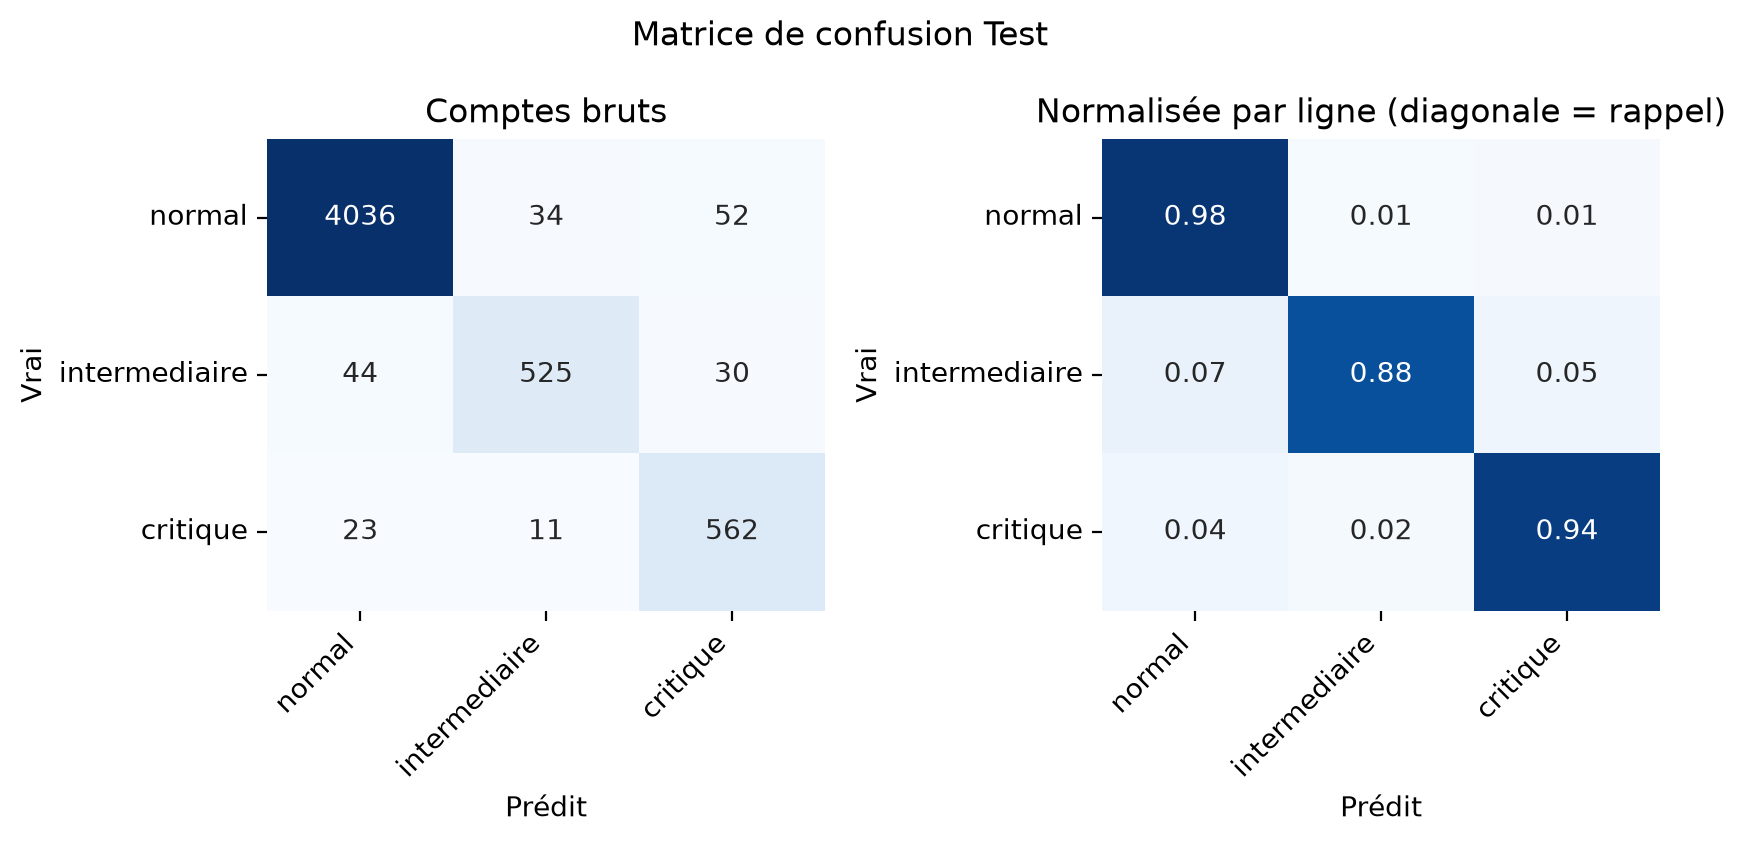
\includegraphics[width=\linewidth]{report/baseline_confusion_criticality.png}
  \caption{Matrice de confusion de test sur la criticité (comptes bruts et normalisée par ligne).}
  \label{fig:baseline-confusion-criticality}
\end{figure}

\begin{figure}[H]
  \centering
  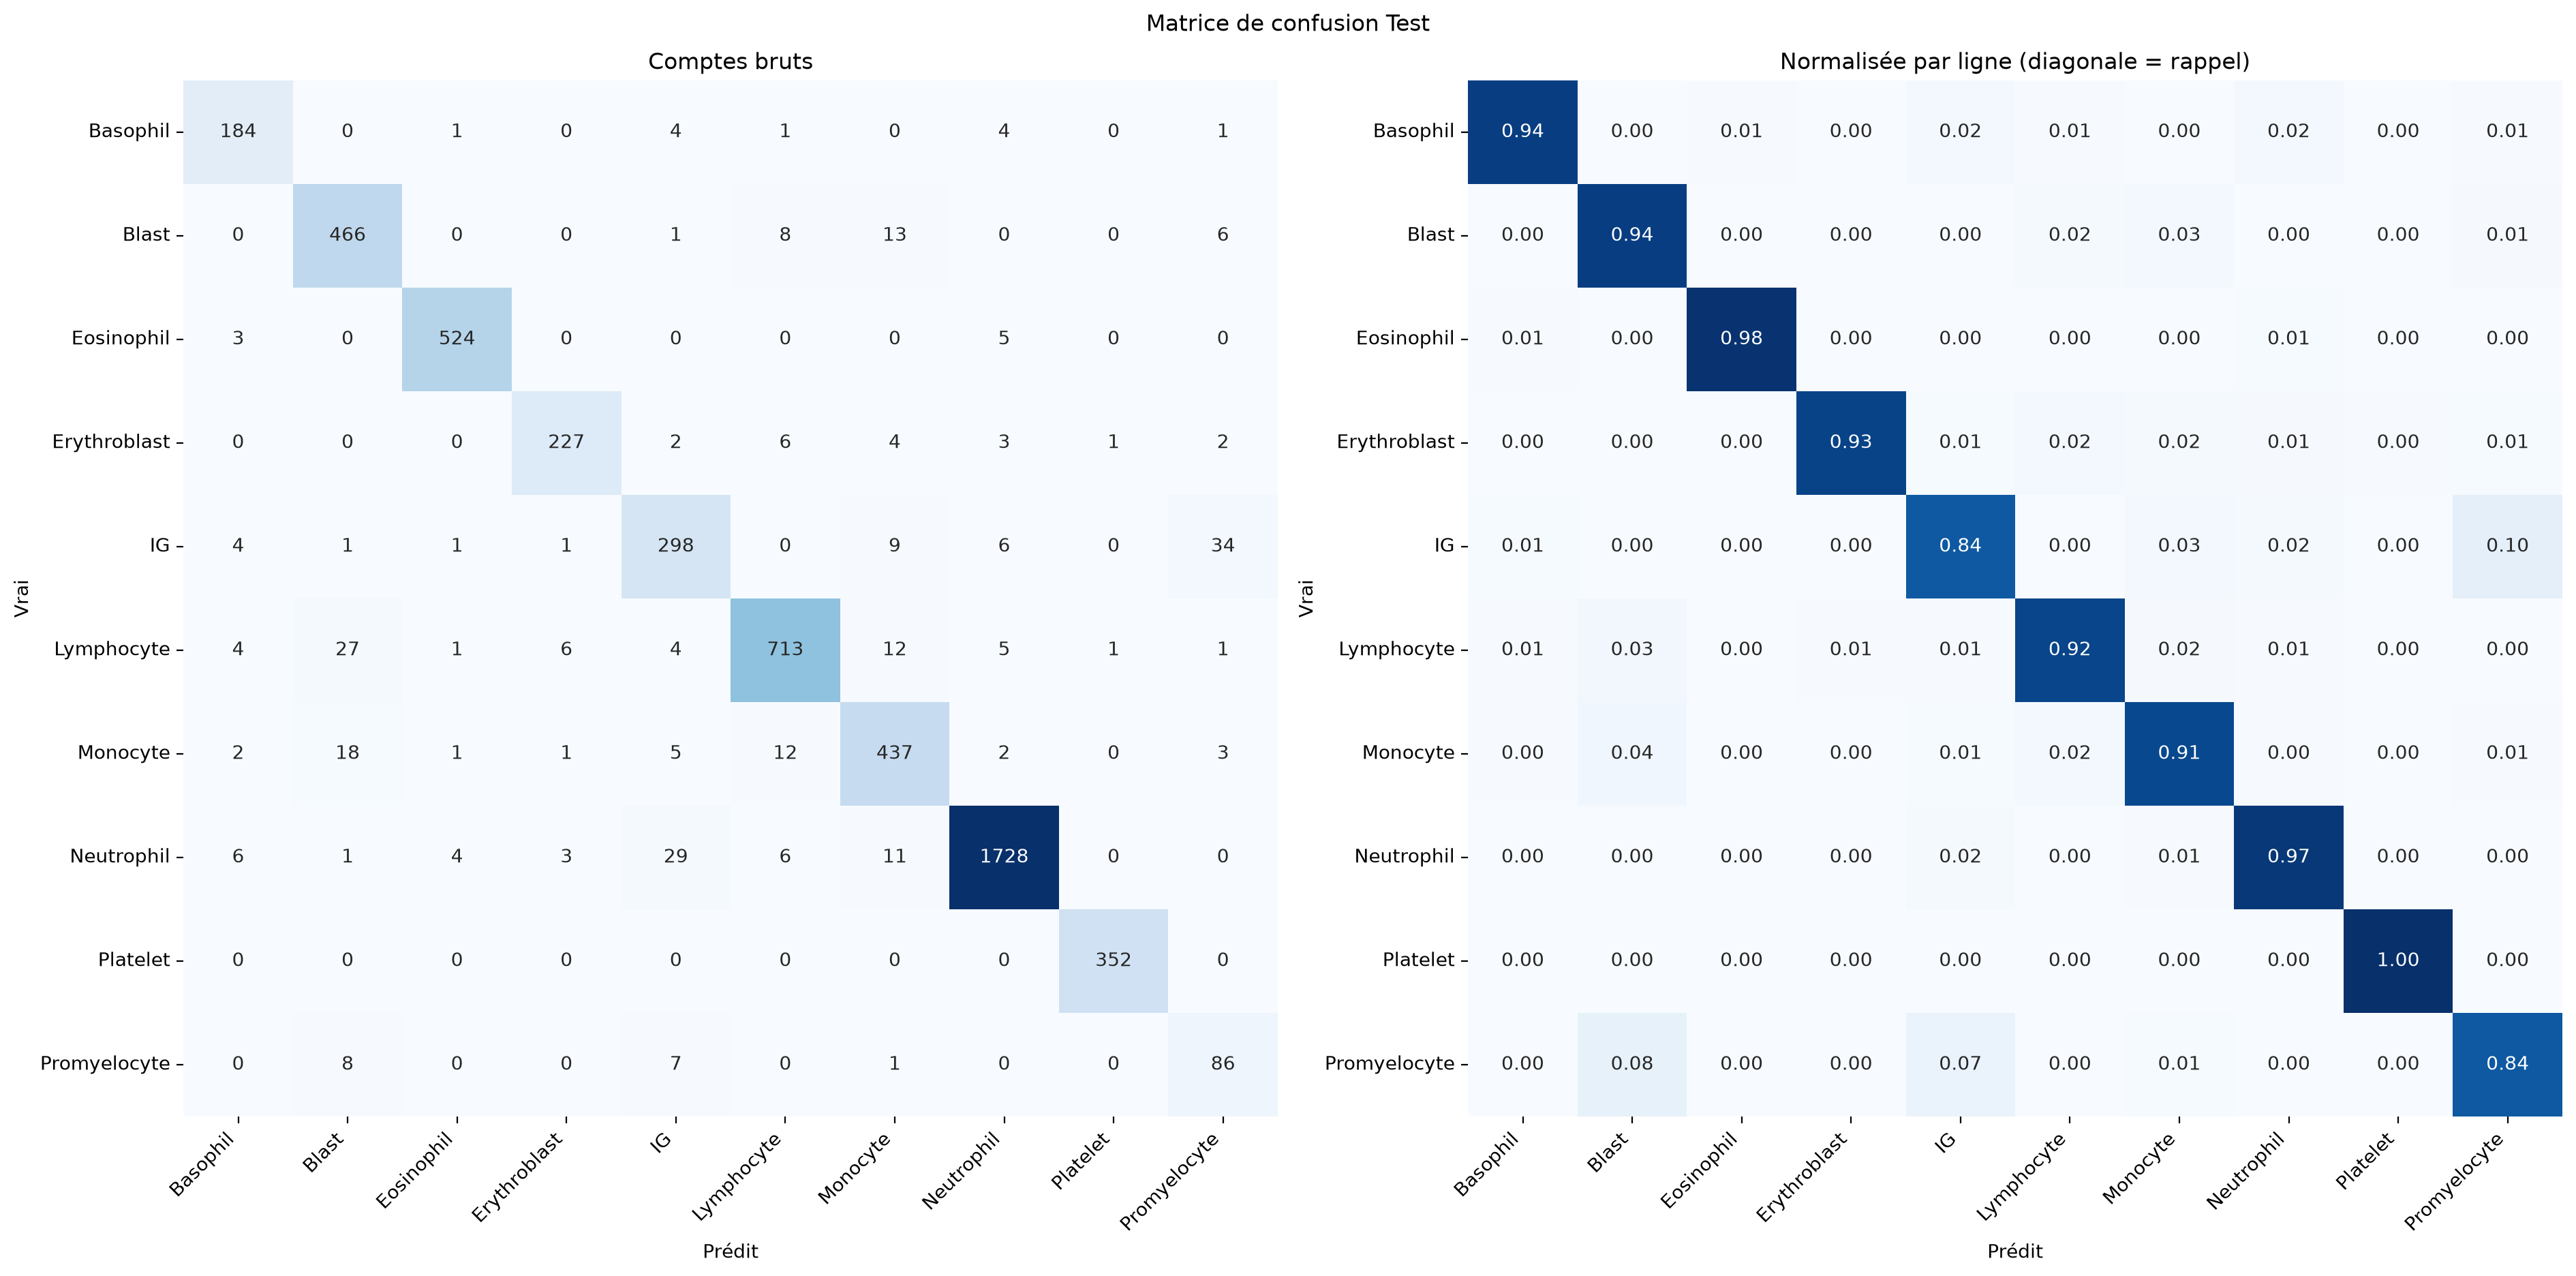
\includegraphics[width=\linewidth]{report/baseline_confusion_type.png}
  \caption{Matrice de confusion de test sur les types de cellules (comptes bruts et normalisée par ligne).}
  \label{fig:baseline-confusion-type}
\end{figure}

Sur \texttt{criticality} (figure~\ref{fig:baseline-confusion-criticality}), la confusion cliniquement dangereuse critique$\to$normal reste rare (23 images sur 596, soit 3,9\,\%) et près de trois fois moins fréquente que normal$\to$critique (52 sur 4\,122, 1,3\,\%), cohérent avec la matrice de coût qui pénalise fortement la première direction.
Sur \texttt{type} (figure~\ref{fig:baseline-confusion-type}), l'essentiel des erreurs reste \emph{intra-palier} : le promyélocyte (rappel 0,84, la classe la plus faible) est majoritairement confondu avec le blaste (8 images) et les granulocytes immatures (7 images), deux classes elles-mêmes critiques ou intermédiaires, jamais avec une classe normale.
Le rappel critique de \emph{validation} de ce run précis (0,782) est nettement inférieur à l'estimation multi-seed du grid (0,910, tableau~\ref{tab:imbalance-grid}) tandis que le \emph{test} (0,843) retombe entre les deux : une illustration concrète de la variance inter-seed déjà signalée (\hyperref[sec:limites-loss]{limites de la perte}) plutôt qu'une dégradation réelle du modèle.

\begin{figure}[H]
  \centering
  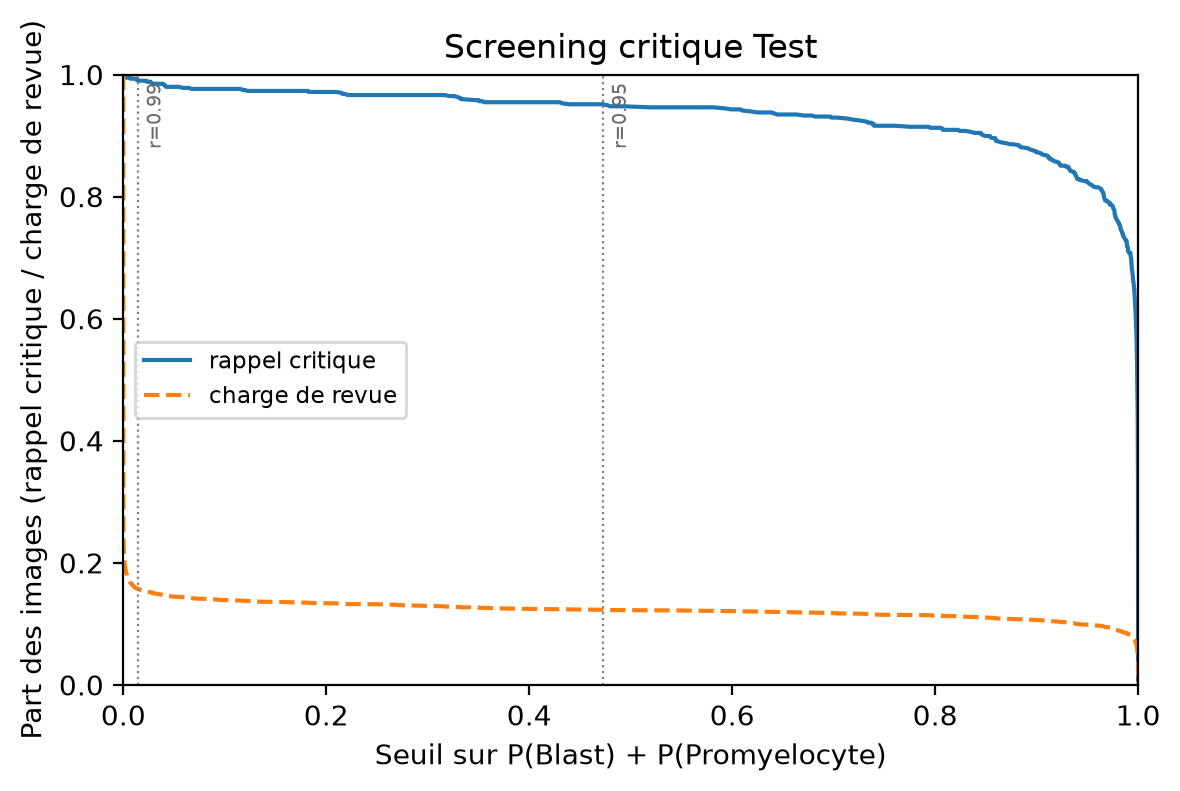
\includegraphics[width=0.75\linewidth]{report/baseline_critical_screening_type.png}
  \caption{Rappel critique et charge de revue (part des images envoyées en relecture) en fonction du seuil sur $P(\text{blaste}) + P(\text{promyélocyte})$.
Les repères verticaux marquent les seuils les plus stricts atteignant un rappel de 0,99 et 0,95.}
  \label{fig:baseline-critical-screening}
\end{figure}

Le seuil par défaut (\emph{argmax}) ne suffit pas à atteindre la cible de rappel critique de 0,95 (\S~\ref{sub:metriques}), mais un ajustement de seuil en post-traitement, déjà anticipé au \hyperref[sec:limites-loss]{limites de la perte}, s'en approche à moindre coût (figure~\ref{fig:baseline-critical-screening}).
En abaissant le seuil de décision sur la masse de probabilité critique $P(\text{blaste}) + P(\text{promyélocyte})$ à $\approx 0,48$, le rappel critique atteint 0,95 (précision $\approx$ 0,87) en n'envoyant que $\approx$ 12\,\% des 5\,317 images de test en revue supplémentaire.
Pousser jusqu'à un rappel de 0,99 demande un seuil beaucoup plus bas ($\approx 0,01$), pour une charge de revue qui reste modérée ($\approx$ 16\,\%, précision $\approx$ 0,71) : la plupart des 596 cellules critiques du test sont déjà bien identifiées, et il suffit d'un seuil nettement plus permissif pour en récupérer la quasi-totalité.
Un noyau dur de 5 cellules critiques (sur 596) reçoit toutefois un score quasi nul quel que soit le seuil : un rappel strictement parfait (1,00) exigerait de faire descendre le seuil jusqu'à 0, envoyant alors 36\,\% des images en revue.

\begin{figure}[H]
  \centering
  \begin{subfigure}{0.48\linewidth}
    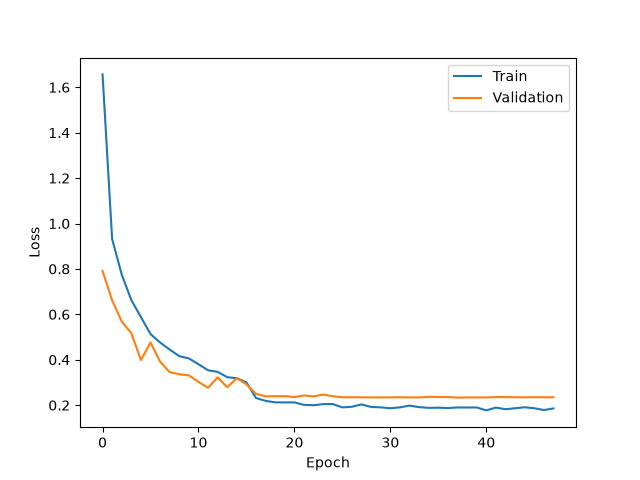
\includegraphics[width=\linewidth]{report/baseline_training_loss_type.png}
    \caption{Perte train / validation.}
  \end{subfigure}
  \hfill
  \begin{subfigure}{0.48\linewidth}
    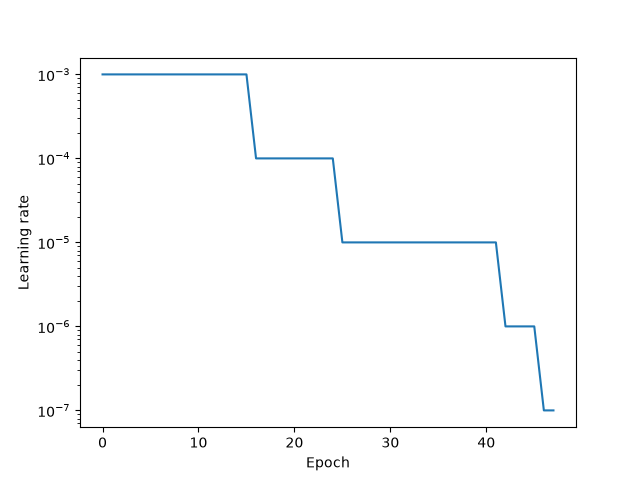
\includegraphics[width=\linewidth]{report/baseline_training_lr_type.png}
    \caption{Taux d'apprentissage.}
  \end{subfigure}
  \caption{Courbes d'entraînement (échelle log pour le taux d'apprentissage).}
  \label{fig:baseline-training-curves}
\end{figure}

La figure~\ref{fig:baseline-training-curves} illustre concrètement le scheduler et l'early stopping décrits au \S~\ref{sec:optimizer} : la perte de validation stagne dès l'époque $\approx$15, provoquant quatre réductions successives du taux d'apprentissage ($10^{-3} \to 10^{-7}$) par \texttt{plateau}, jusqu'à l'arrêt anticipé à l'époque 48 sur un budget de 50 ; la perte d'entraînement, elle, continue de baisser légèrement, signe d'un léger surapprentissage contenu par la restauration des meilleurs poids.

Ces résultats sont \textbf{encourageants} pour un modèle aussi simple : sans poids pré-entraînés ni \emph{batch-norm}, la \emph{baseline} dépasse déjà 0,92 de F1 macro sur les deux tâches, et l'ajustement de seuil montre qu'une cible de rappel critique de 0,95 est à sa portée.
Elle reste toutefois limitée par sa structure (99\,\% des paramètres concentrés dans une couche dense, aucune robustesse à la position de la cellule, \S~\ref{sec:modele-avance} ci-après) et par le coût du seuillage : atteindre 0,99 de rappel exige un seuil très permissif, révélateur d'un noyau dur d'erreurs (5 cellules critiques sur 596) que le réglage du seuil seul ne résorbe pas.
La section suivante explore donc des architectures plus équilibrées, dans les mêmes conditions d'entraînement, pour chercher ce que la structure du réseau peut encore apporter au-delà du rééquilibrage de la perte et de l'échantillonnage.

\subsubsection{Modèle avancé}
\label{sec:modele-avance}

La \emph{baseline} constitue un point de départ volontairement simple.
Son analyse met cependant en évidence une faiblesse importante : près de 99\,\% de ses paramètres sont concentrés dans la première couche entièrement connectée, tandis que la partie convolutive ne représente qu'une faible proportion du modèle.
Cette organisation limite notamment la capacité du réseau à construire une représentation compacte des cellules et le rend sensible à leur position dans l'image.

L'étape suivante consiste donc à rechercher une architecture plus équilibrée, sans chercher immédiatement à augmenter fortement la complexité du réseau.
L'objectif est plutôt d'identifier les éléments architecturaux qui apportent réellement un bénéfice dans les conditions du projet.

\paragraph{Questions expérimentales}

L'étude est organisée autour de plusieurs choix structurants de l'architecture.
Ils sont directement motivés par les limites observées sur la \emph{baseline} :

\begin{itemize}
\item \textbf{Profondeur du réseau :} une augmentation du nombre de blocs ou de couches convolutives permet-elle d'améliorer la représentation des cellules ?
\item \textbf{Nombre de canaux :} une capacité de représentation plus importante apporte-t-elle un gain mesurable, ou conduit-elle principalement à augmenter la complexité ?
\item \textbf{Taille des noyaux :} les noyaux $5\times5$ permettent-ils de mieux exploiter le contexte local qu'une succession de noyaux $3\times3$ ?
\item \textbf{Batch Normalization :} son ajout améliore-t-il la stabilité et les performances de l'apprentissage ?
\item \textbf{Global Average Pooling :} peut-il remplacer le \emph{flatten} massif de la \emph{baseline} et réduire la dépendance à la position de la cellule ?
\item \textbf{Classifieur :} une tête plus profonde apporte-t-elle une capacité supplémentaire utile après l'extraction des caractéristiques ?
\end{itemize}

L’objectif n’est donc pas de trouver le réseau le plus complexe, mais une architecture qui apporte un gain sans ajouter de complexité inutile.

\begin{figure}[H]
\centering
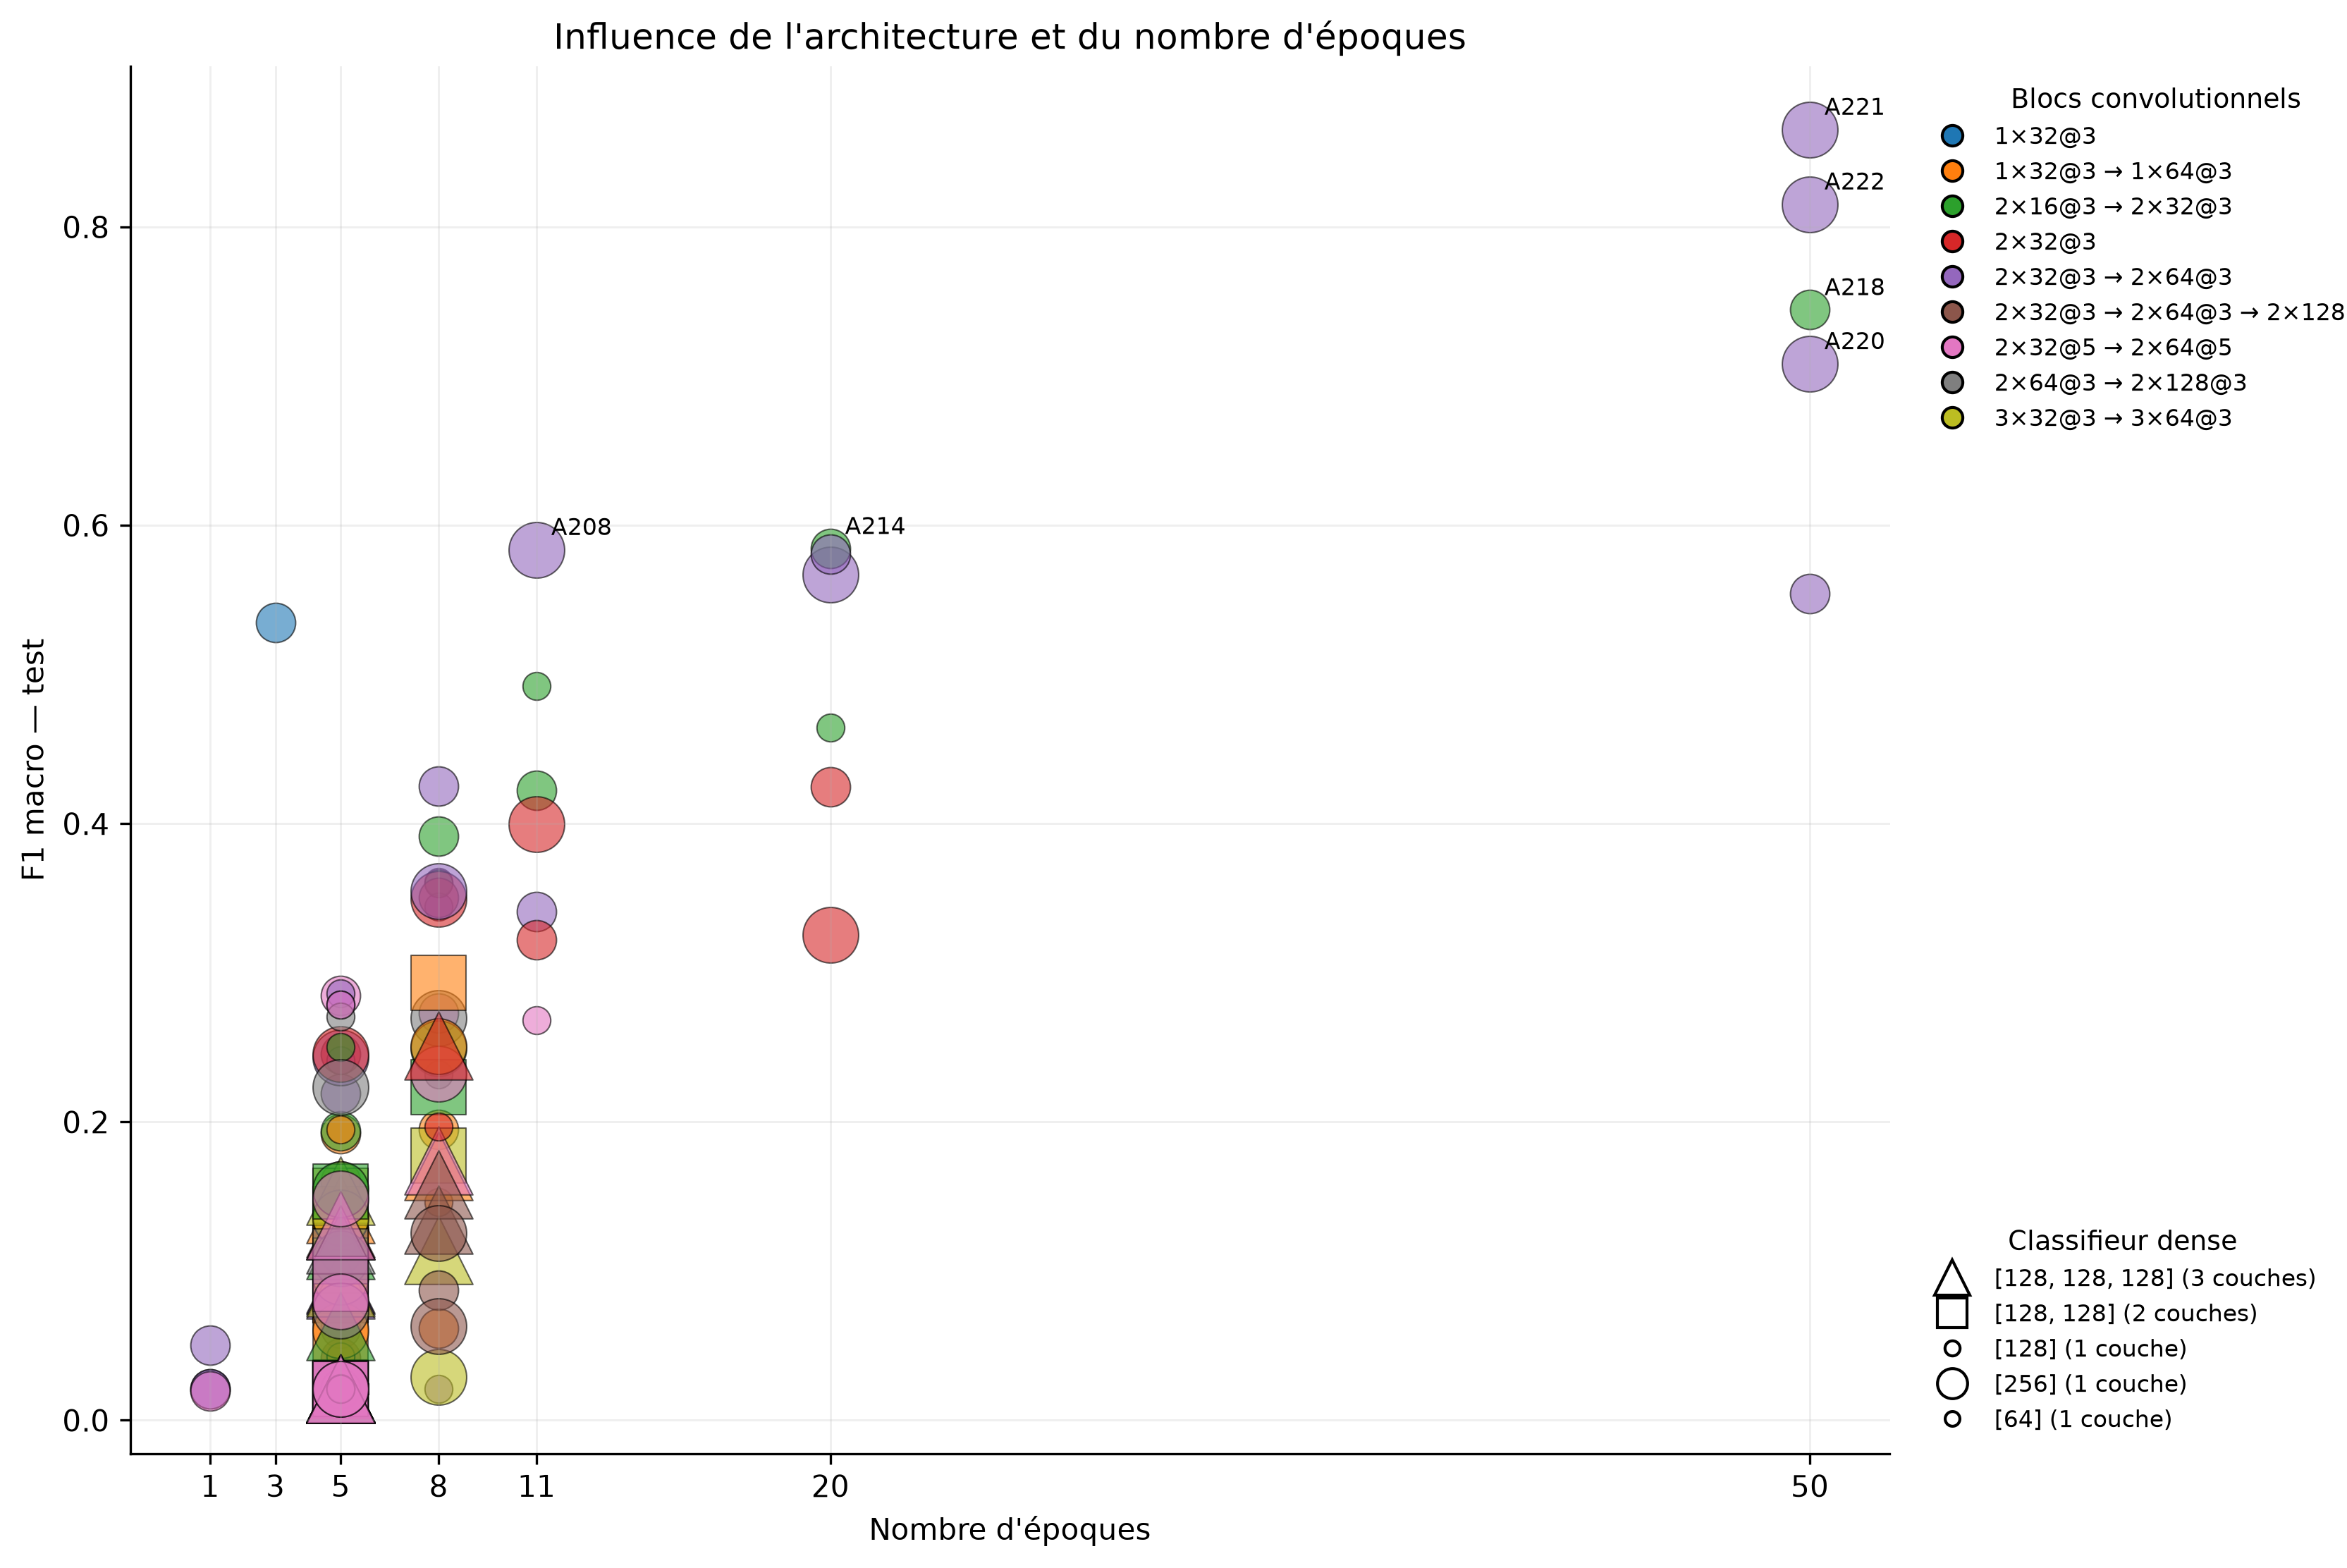
\includegraphics[width=0.92\linewidth]{figures/report/comparaison_blocks_classifieur_epochs.png}
\caption{Organisation de l'exploration architecturale.
La \emph{baseline} sert de point de départ ; les principaux choix structurants sont ensuite comparés séparément avant de sélectionner une architecture de référence.}
\label{fig:architecture-exploration}
\end{figure}

\paragraph{Protocole de comparaison}

Au total, \textbf{79 entraînements} ont été réalisés pour explorer ces différentes configurations.
Les expérimentations sont conduites dans un cadre d'entraînement commun afin de limiter l'influence des paramètres qui ne concernent pas directement l'architecture.

Le \textit{batch size}, le nombre d'époques, le taux d'apprentissage, le \textit{weight decay}, l'optimiseur, le scheduler, la fonction de perte, la graine aléatoire et les transformations d'augmentation sont maintenus selon un protocole commun.
Leur optimisation fait l'objet d'expérimentations distinctes.

Cette séparation est importante : elle permet d'attribuer les différences observées principalement à la structure du réseau plutôt qu'à une combinaison particulière de paramètres d'entraînement.

Les modèles sont comparés principalement à partir du \textbf{F1-score macro}.
Le F1 macro donne le même poids aux différentes classes et reste donc adapté au déséquilibre du jeu de données.

\paragraph{Architecture explorée}

Les modèles reposent sur une même organisation générale :

$$
\text{image} \rightarrow
\text{blocs convolutifs} \rightarrow
\text{représentation} \rightarrow
\text{classifieur} \rightarrow
\text{10 classes}.
$$

Les blocs convolutifs font varier trois dimensions principales : leur nombre, leur profondeur et leur nombre de canaux.
La majorité des configurations utilisent des noyaux $3\times3$, avec une configuration utilisant des noyaux $5\times5$ afin d'explorer l'influence d'un champ réceptif plus large.

Deux modifications sont particulièrement liées aux limites de la \emph{baseline}.
La première concerne la \textit{Batch Normalization}, ajoutée après les convolutions afin d'évaluer son influence sur l'apprentissage.
La seconde concerne le \textit{Global Average Pooling}, qui permet de remplacer l'aplatissement de la carte de caractéristiques par une représentation beaucoup plus compacte avant le classifieur.

Enfin, plusieurs têtes de classification sont comparées, depuis une structure simple jusqu'à des classifieurs comportant plusieurs couches entièrement connectées.

\paragraph{Résultats}

Les résultats ne montrent pas que rendre le réseau plus complexe améliore systématiquement les performances.
L'augmentation du nombre de blocs convolutifs ou de leur profondeur ne conduit pas systématiquement à une amélioration du F1 macro.
Les architectures les plus complexes ne présentent donc pas d'avantage général dans les conditions expérimentales considérées.

Une \textbf{profondeur modérée} semble au contraire constituer un compromis plus adapté.
L'augmentation du nombre de canaux présente une tendance similaire : une capacité intermédiaire semble suffisante pour représenter les caractéristiques utiles à la classification, tandis qu'une augmentation importante de cette capacité n'apporte pas de gain systématique.

La \textbf{Batch Normalization} présente une tendance favorable dans les configurations testées.
Son ajout est associé à de meilleures performances et constitue donc un choix retenu pour la suite.

Le \textbf{Global Average Pooling} présente également une tendance favorable.
Au-delà de son influence sur les performances, il répond directement à une faiblesse identifiée dans la \emph{baseline} : il évite de transformer une carte $64\times27\times27$ en plusieurs dizaines de milliers de valeurs avant la première couche dense.
La représentation transmise au classifieur devient ainsi plus compacte et moins directement dépendante de la position des caractéristiques dans l'image.

Concernant le \textbf{classifieur}, les structures simples obtiennent globalement de meilleurs résultats que les architectures comportant plusieurs couches entièrement connectées.
L'ajout de profondeur après le bloc convolutif ne semble donc pas nécessaire dans les conditions étudiées.

Enfin, une configuration utilisant des noyaux $5\times5$ obtient des résultats encourageants.
Cependant, le nombre d'essais disponibles ne permet pas d'isoler suffisamment l'effet de la taille du noyau pour conclure à un avantage systématique par rapport aux noyaux $3\times3$.

\begin{table}[H]
\centering
\caption{Synthèse des tendances observées lors de l'exploration architecturale.}
\label{tab:architecture-impact}
\begin{tabularx}{\textwidth}{>{\raggedright\arraybackslash}p{3.2cm} >{\raggedright\arraybackslash}X >{\raggedright\arraybackslash}X}
\toprule
\textbf{Choix} & \textbf{Observation} & \textbf{Décision} \\
\midrule

Nombre de blocs
& La complexité supplémentaire n'apporte pas de gain systématique
& Conserver une profondeur modérée \\

Profondeur des blocs
& Les configurations très profondes sont plutôt défavorables
& Privilégier des blocs peu profonds \\

Nombre de canaux
& Une capacité intermédiaire semble suffisante
& Éviter une augmentation excessive des canaux \\

Kernel
& $3\times3$ majoritaire ; un essai $5\times5$ est encourageant
& Conserver $3\times3$ comme référence ; poursuivre l'étude de $5\times5$ si nécessaire \\

Batch Normalization
& Tendance favorable
& Retenue dans l'architecture de référence \\

GAP
& Tendance favorable et réduction importante de la représentation avant le classifieur
& Retenu dans l'architecture de référence \\

Classifieur
& Les structures simples sont globalement favorisées
& Utiliser une tête compacte \\

\bottomrule
\end{tabularx}
\end{table}

\paragraph{Choix de l'architecture de référence}

À l'issue de cette exploration, l'architecture de référence n'est donc pas choisie sur la base de sa complexité maximale, mais sur la base du compromis observé entre capacité et simplicité.

Elle privilégie une \textbf{profondeur modérée}, un \textbf{nombre de canaux intermédiaire}, la \textbf{Batch Normalization}, un \textbf{Global Average Pooling} et un \textbf{classifieur compact}.
Les noyaux $3\times3$ sont conservés comme choix de référence, les résultats disponibles sur $5\times5$ ne permettant pas encore d'établir une conclusion suffisamment robuste.

Cette architecture constitue la nouvelle référence pour la suite des expérimentations.
Elle permet ensuite de comparer plus proprement l'apport du \textit{Transfer Learning}, des stratégies d'entraînement et des autres modifications du modèle, en conservant une architecture maîtrisée comme point de comparaison.

\subsubsection{Transfer Learning}
\label{sec:transfer-learning}

L'exploration précédente conserve un réseau entraîné \emph{from scratch} : ses caractéristiques doivent être apprises intégralement à partir des images du projet.
Le transfert d'apprentissage propose une alternative directement motivée par les limites de la \emph{baseline} (\S~\ref{sec:modele-avance}) : remplacer le tronc convolutif par un extracteur pré-entraîné sur ImageNet, réutilisé et éventuellement ré-affiné pour la classification des cellules sanguines, avec la même tête \emph{global average pooling} + classifieur compact retenue précédemment.
\paragraph{Modèles de référence dans la littérature}
 
La classification de cellules sanguines par transfert d'apprentissage est déjà largement documentée.
\textbf{Matek et al.} \parencite{matek2019nmi} rapportent une reconnaissance « de niveau humain » sur la discrimination blaste / non-blaste avec un \textbf{ResNeXt-50} pré-entraîné sur ImageNet, directement sur Matek-19 (LMU), l'une des deux sources fusionnées dans ce projet ($\approx$90\,\% d'accuracy) : c'est le \emph{benchmark} clinique historique sur les blastes.
\textbf{Acevedo et al.} \parencite{acevedo2019cnn} obtiennent $\approx$96\,\% sur PBC avec \textbf{VGG-16} et \textbf{InceptionV3} affinés.
Plus récemment, plusieurs travaux sur PBC seul (8 classes, taxonomie plus fine que nos 10 classes fusionnées) rapportent 98--98,6\,\% avec des architectures \textbf{EfficientNet-B0/B3}, \textbf{EfficientNetV2-S} et \textbf{DenseNet-121} \parencite{asghar2024tenclasses,asghar2023allbloodcell}, tandis qu'une revue dédiée aux \emph{Vision Transformers} sur ce type d'images les juge compétitifs face aux CNN classiques, à condition de données et d'augmentation suffisantes \parencite{abouali2023wbcvit}.

Plutôt que d'explorer arbitrairement l'espace des architectures, la grille de ce projet reprend donc les principaux modèles utilisés dans cette littérature : \textbf{ResNet-50} (comparable au ResNeXt-50 de Matek et al.), \textbf{EfficientNet-B0}, \textbf{EfficientNetV2-S} et \textbf{DenseNet-121} (CNN les plus cités sur PBC), \textbf{ViT-Base/16} et \textbf{Swin-Tiny} (\emph{Vision Transformers}), en y ajoutant \textbf{ConvNeXt-Tiny}, architecture CNN plus récente non directement couverte par ces travaux mais représentative de la génération suivant EfficientNet.
Deux pistes de la même littérature n'ont en revanche pas pu être testées faute de budget de calcul : \textbf{DinoBloom} \parencite{koch2024dinobloom}, un modèle de fondation ViT pré-entraîné en auto-supervisé (DINOv2) sur plus de 380\,000 images réparties sur 13 jeux d'hématologie incluant Matek-19, dont les variantes vont de 22\,M (DinoBloom-S) à 1,1\,milliard de paramètres (DinoBloom-G) ; et les approches d'adaptation de domaine explicite (DANN \parencite{ganin2016dann} ou alignement de features cross-site \parencite{gao2025danet,sadafi2023continual}) qui viseraient directement le \emph{domain gap} PBC/LMU déjà signalé (\S~\ref{sec:pre-processing-feature-engineering}), mais demanderaient une implémentation et une validation dédiées, hors du périmètre de ce projet.

\paragraph{Caractéristiques des backbones testés}

Le tableau~\ref{tab:transfer-backbones} résume l'architecture et la taille des 7 backbones retenus.

\begin{table}[H]
  \centering
  \small
  \renewcommand{\arraystretch}{1.15}
  \begin{tabularx}{\textwidth}{@{} l X r @{}}
    \toprule
    Backbone & Architecture & Paramètres \\
    \midrule
    ResNet-50         & CNN à connexions résiduelles (\emph{skip connections}), 50 couches & 23,5 M \\
    EfficientNet-B0   & CNN à mise à l'échelle composée (profondeur / largeur / résolution) & 4,0 M \\
    DenseNet-121      & CNN à connexions denses (chaque couche reçoit les sorties de toutes les précédentes) & 7,0 M \\
    ConvNeXt-Tiny     & CNN « modernisé » (grands noyaux, LayerNorm, GELU, recette d'entraînement inspirée des Transformers) & 27,8 M \\
    ViT-Base/16       & \emph{Vision Transformer} pur, patches $16\times16$, auto-attention globale & 85,8 M \\
    EfficientNetV2-S  & CNN, blocs \emph{Fused-MBConv} puis \emph{MBConv}, entraînement progressif de la résolution & $\approx$21 M \\
    Swin-Tiny         & Transformer hiérarchique à fenêtres glissantes (attention locale + décalage) & $\approx$28 M \\
    \bottomrule
  \end{tabularx}
  \caption{Backbones testés (poids ImageNet, \texttt{timm}) : architecture et nombre de paramètres entraînables en fine-tuning complet.
Valeurs mesurées sur nos runs pour les 5 premiers backbones ; approximatives (architecture publiée) pour EfficientNetV2-S et Swin-Tiny, dont le nombre de paramètres n'a pas été historisé dans le sweep complémentaire.}
  \label{tab:transfer-backbones}
\end{table}

\paragraph{Intégration dans le pipeline}

Le framework a été modifié pour permettre de charger n'importe quel backbone supporté par \textbf{timm} \parencite{wightman2019timm}, sans classifieur mais avec un \emph{global average pooling}.

On peut ensuite configurer la tête de classification, soit juste une couche de sortie, soit avec des couches cachées configurables.

En utilisant \textbf{timm}, on peut choisir de charger les modèles déjà pré-entraînés ou de les initialiser de manière aléatoire.

Dans le cas où les modèles sont pré-entraînés, on peut choisir de n'entraîner que la tête de classification, de dégeler seulement certaines couches ou bien la totalité du modèle.
Si certaines couches sont dégelées, leurs paramètres sont déjà entraînés, tandis que la tête est initialisée aléatoirement.
Utiliser le même \emph{learning rate} pour les deux risque d'être trop violent pour les couches déjà entraînées, il est donc possible de configurer un multiplicateur entre les deux groupes de paramètres.

Enfin, dans les étapes de pré-traitement, on normalise les images en utilisant soit les statistiques de notre dataset ou bien celles d'ImageNet.

\paragraph{Grilles de recherche}

Deux recherches par grille ont été effectuées pour comparer 7 backbones pré-entraînés sur ImageNet : ResNet-50, EfficientNet-B0, DenseNet-121, ConvNeXt-Tiny, ViT-Base/16 (patch 16), EfficientNetV2-S et Swin-Tiny, sur un sous-ensemble de 15\,000 images (budget de 10 époques, sans \emph{early stopping}), en faisant varier six blocs de configuration :

\begin{itemize}
\item \textbf{G1 : linear probing} : backbone entièrement gelé, tête linéaire.
\item \textbf{G2 : fine-tuning complet} : backbone dégelé, sweep du multiplicateur de LR du backbone (\texttt{backbone\_lr\_mult} $\in \{0{,}01\,;\ 0{,}1\,;\ 1\}$, LR backbone = LR tête $\times$ mult).
\item \textbf{G3 : gel partiel} : dégel des 1 ou 2 derniers blocs seulement.
\item \textbf{G4 : contrôle avec poids aléatoires} : mêmes architectures, initialisation aléatoire au lieu des poids ImageNet.
\item \textbf{G5 : normalisation} : stats de normalisation ImageNet vs stats calculées sur le dataset harmonisé.
\item \textbf{G6 : architecture de la tête} : profondeur (linéaire / 1 couche / 2 couches) et \emph{dropout} (0 / 0,3), à backbone gelé.
\end{itemize}

La première grille s'est concentrée sur les backbones ResNet-50, EfficientNet-B0, DenseNet-121, ConvNeXt-Tiny, ViT-Base/16 (patch 16) et a utilisé une taille de batch de 32, tandis que la seconde a fait tourner seulement certaines configurations mais sur tous les backbones, et a pu tourner avec des batchs de 124.
La différence de taille de batch n'est pas anecdotique, sur les backbones communs et à configurations identiques, les scores avec des batchs de 124 sont systématiquement inférieurs de quelques points.
Cet effet est à garder en tête pour toutes comparaison entre les runs.

Au total, 93 entraînements ont été menés sur la première grille ($\approx$19h12 cumulées) et 50 sur la seconde ($\approx$8h12 cumulées).

\paragraph{Stratégie de gel et apport du pré-entraînement}

\begin{figure}[H]
\centering
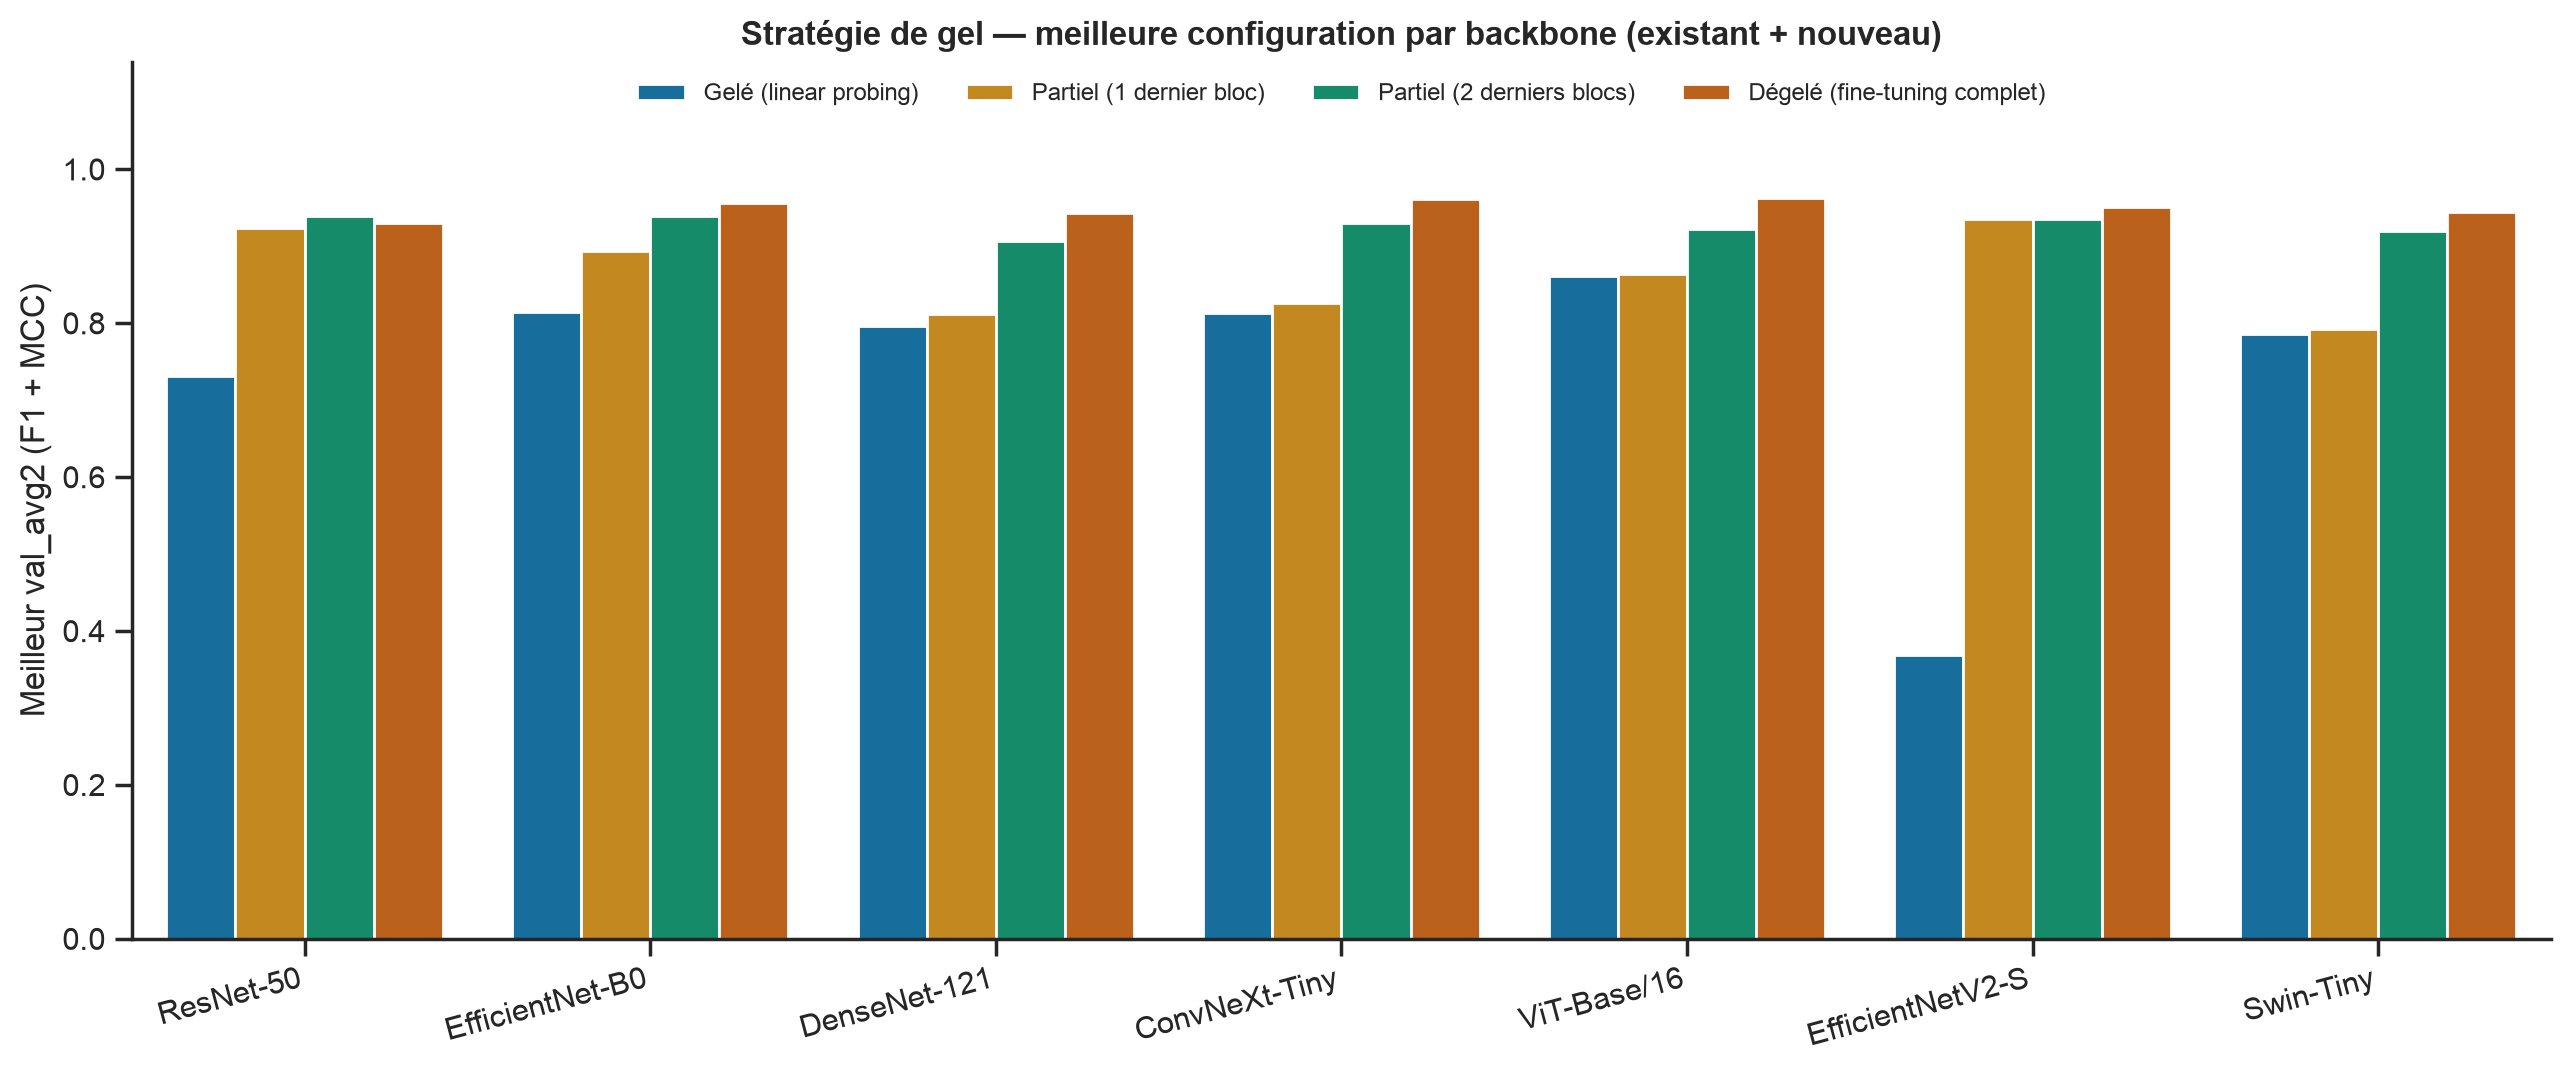
\includegraphics[width=\linewidth]{report/transfer_grid_freeze_strategy.png}
\caption{Meilleur score de validation (F1 macro + MCC) par backbone, selon la stratégie de gel (linear probing, gel partiel, fine-tuning complet), sur les 7 backbones.}
\label{fig:transfer-freeze-strategy}
\end{figure}

Le dégel complet du backbone (figure~\ref{fig:transfer-freeze-strategy}) domine sur les 7 architectures (0,93 à 0,96), avec un gain net mais décroissant selon la stratégie : le gel partiel apporte un premier gain progressif (0,79 à 0,94 selon le backbone et le nombre de blocs dégelés), et le linear probing plafonne généralement entre 0,73 et 0,86, à l'exception d'EfficientNetV2-S, dont le score s'effondre à 0,37 en linear probing avant de remonter à 0,94 dès qu'un seul bloc est dégelé ; cette anomalie isolée à ce backbone (tête, normalisation ou spécificité de l'architecture) resterait à investiguer.
Contrairement à un transfert « classique » où le backbone gelé suffit déjà à bien discriminer les classes, les cellules sanguines profitent ici d'un ré-apprentissage complet des caractéristiques bas niveau, cohérent avec un domaine visuel (cytologie) très éloigné d'ImageNet.

\begin{figure}[H]
\centering
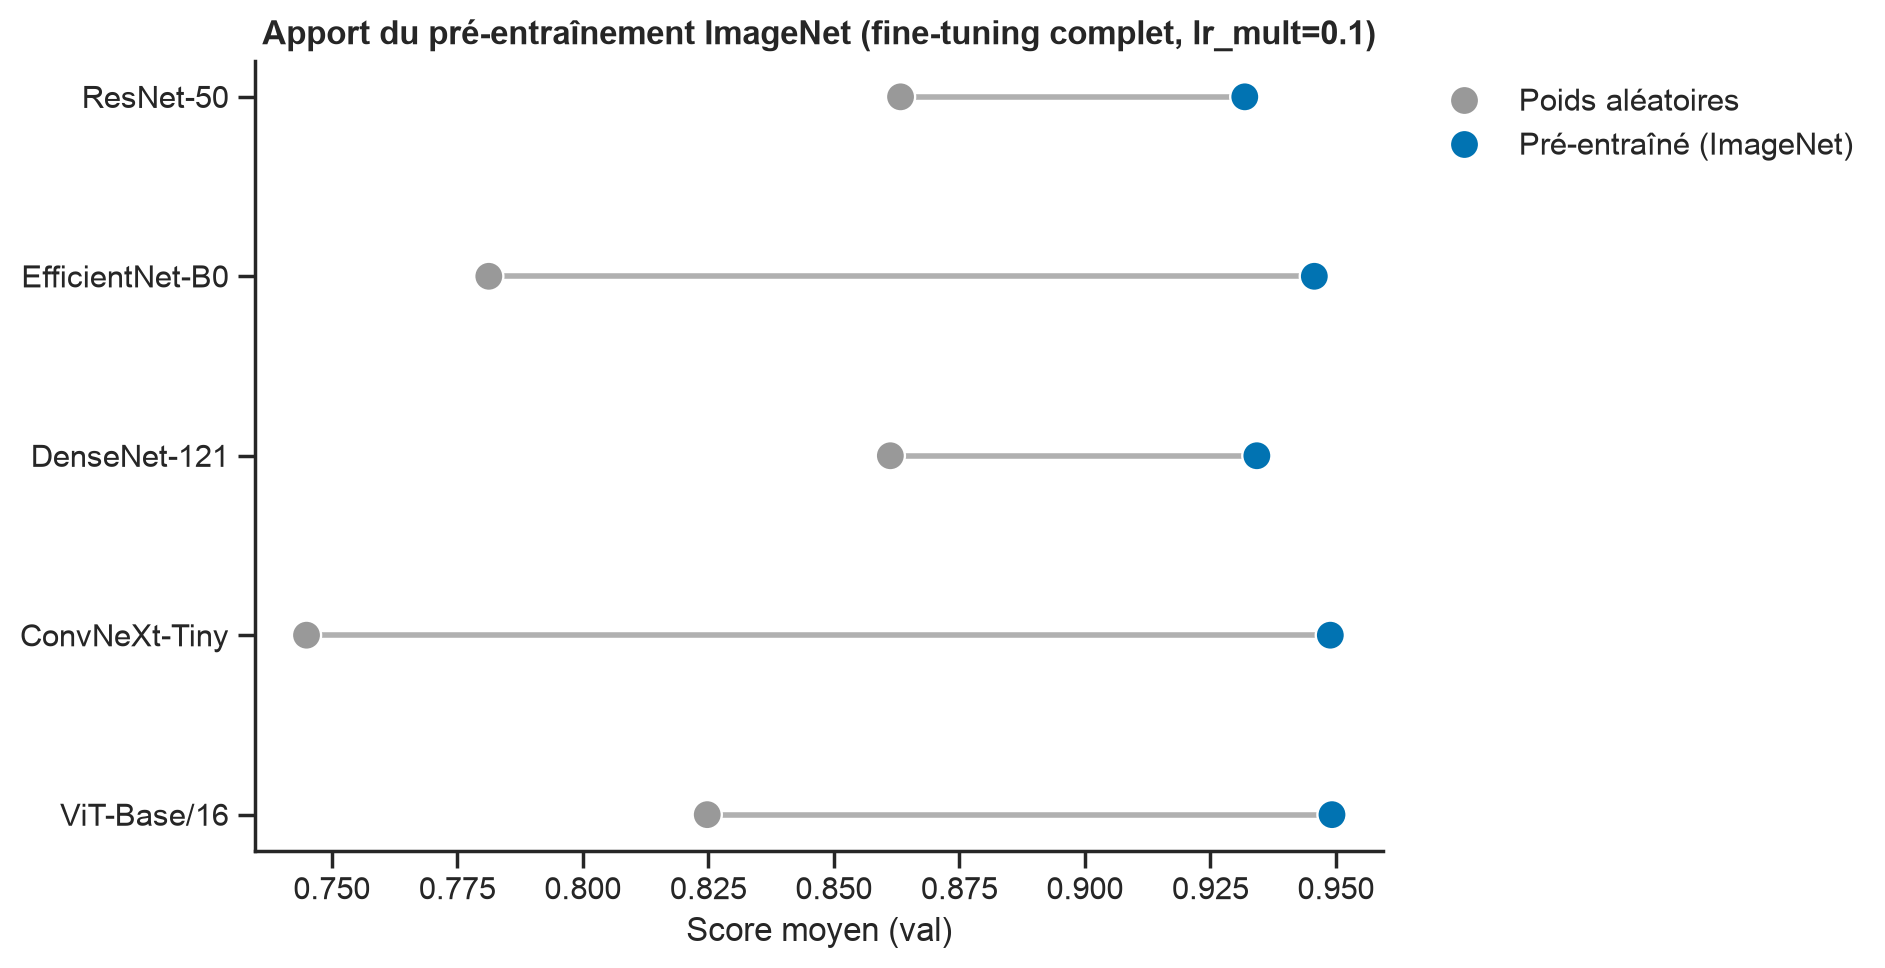
\includegraphics[width=0.85\linewidth]{report/transfer_grid_pretrained.png}
\caption{Apport des poids ImageNet par rapport à une initialisation aléatoire, à stratégie de fine-tuning identique (\texttt{backbone\_lr\_mult}=0,1).}
\label{fig:transfer-pretrained}
\end{figure}

Le pré-entraînement ImageNet reste toutefois indispensable (figure~\ref{fig:transfer-pretrained}) : à stratégie de dégel identique, les poids aléatoires perdent entre 0,10 (ResNet-50) et 0,20 (ConvNeXt-Tiny) de score moyen par rapport aux poids ImageNet.
Même entièrement ré-entraîné, le backbone bénéficie donc d'un point de départ informatif que 15\,000 images ne suffiraient pas à reconstruire seules.

\paragraph{Normalisation et architecture de la tête}

Les stats de normalisation ImageNet devancent systématiquement celles calculées sur le dataset harmonisé (de --0,01 à --0,02 pour les CNN, jusqu'à --0,11 pour ConvNeXt-Tiny).
Ce résultat est cohérent avec des poids pré-entraînés sur ImageNet, les stats d'ImageNet sont retenues pour la suite.

L'architecture de la tête (G6, à backbone gelé) n'apporte en revanche pas de tendance uniforme : une couche cachée avec \emph{dropout} améliore légèrement le F1 macro pour certains backbones (ViT : 0,864 $\to$ 0,879 ; DenseNet-121 : 0,800 $\to$ 0,828) mais reste marginale comparée à l'effet du dégel complet ($\approx$+0,10 à +0,15).
Une tête linéaire simple est donc conservée pour la suite dans la plupart des cas, dans la continuité de la conclusion de \S~\ref{sec:modele-avance} (à l'exception de ConvNeXt-Tiny, qui utilise une couche cachée de 256).

\paragraph{Backbones retenus}

Une fois le fine-tuning complet choisi comme stratégie, le classement sur le score F1 macro + MCC se resserre fortement : ViT-Base/16 (0,962), ConvNeXt-Tiny (0,961), EfficientNet-B0 (0,956) et EfficientNetV2-S (0,951) sont proches, suivis de DenseNet-121 et Swin-Tiny (0,944 chacun), nettement devant ResNet-50 (0,931).
On choisit donc d'effectuer des runs plus poussés sur ViT-Base/16, ConvNeXt-Tiny, EfficientNet-B0 et DenseNet-121, ce dernier choisi pour son bon rapport score/nombre de paramètres et les autres écartés surtout pour une question de budget de calcul.

\paragraph{Runs finaux}

Les backbones retenus (EfficientNet-B0, DenseNet-121, ViT-Base/16 et ConvNeXt-Tiny) sont ré-entraînés une fois chacun sur le jeu complet (35\,457 images, fine-tuning complet, budget de 100 époques, \emph{scheduler} \texttt{plateau}, \emph{early stopping} de patience 10), avec leur meilleure configuration individuelle (\texttt{backbone\_lr\_mult} et optimiseur propres à chaque backbone, tête linéaire, sauf ConvNeXt-Tiny qui utilise une couche cachée de 256) puis évalués sur le test.
Les résultats obtenus sur les principales métriques sont présentés dans le tableau \ref{tab:transfer-resultats-finaux}.

\begin{table}[H]
  \centering
  \renewcommand{\arraystretch}{1.15}
  \resizebox{\textwidth}{!}{%
  \begin{tabular}{@{}lrrrrrrrr@{}}
    \toprule
    Backbone & Époques & Accuracy & F1 macro & MCC & Top-3 acc. & AP screening & Rappel crit. (grp.) & Rappel crit. (min.) \\
    \midrule
    EfficientNet-B0 & 14 & 0,949 & 0,934 & 0,949 & 0,957 & 0,970 & 0,956 & 0,931 \\
    DenseNet-121    & 34 & 0,959 & 0,949 & 0,961 & 0,997 & 0,979 & 0,968 & 0,902 \\
    ViT-Base/16      & 22 & 0,955 & 0,944 & 0,958 & 0,965 & 0,977 & 0,956 & 0,873 \\
    ConvNeXt-Tiny    & 19 & 0,962 & 0,949 & 0,961 & 0,998 & 0,971 & 0,963 & 0,922 \\
    \bottomrule
  \end{tabular}%
  }
  \caption{Métriques de test des runs finaux \emph{transfer learning} (tâche \texttt{type}, 10 classes).
Le rappel critique groupé (\texttt{grouped\_critical\_recall}) et le rappel minimum \emph{par classe} (\texttt{min\_critical\_recall}, promyélocyte) sont définis comme au tableau~\ref{tab:baseline-resultats-finaux}.}
  \label{tab:transfer-resultats-finaux}
\end{table}

Les 4 modèles dépassent nettement la \emph{baseline} (F1 macro 0,916, rappel critique minimum 0,843, tableau~\ref{tab:baseline-resultats-finaux}) sur toutes les métriques, à l'exception du \emph{top-3 accuracy} déjà proche du plafond pour les deux approches.
\textbf{ConvNeXt-Tiny et DenseNet-121} obtiennent des performances quasi identiques (F1 macro 0,949 pour les deux, MCC 0,961) et se disputent la première place selon la métrique : ConvNeXt-Tiny devance légèrement sur l'accuracy (0,962 contre 0,959) et le \emph{top-3 accuracy} (0,998 contre 0,997), tandis que DenseNet-121 reste en tête sur l'AP de criticité (0,979 contre 0,971) et le rappel critique groupé (0,968 contre 0,963).
Les deux devancent nettement ViT-Base/16 malgré un nombre de paramètres entraînables inférieur (28,0 M pour ConvNeXt-Tiny et 7,0 M pour DenseNet-121, contre 85,8 M pour ViT-Base/16) : une confirmation supplémentaire, dans la continuité de \S~\ref{sec:modele-avance}, que la taille du modèle ne garantit pas la meilleure performance.
Le rappel critique minimum par classe reste l'indicateur le plus irrégulier : EfficientNet-B0, pourtant le modèle le plus faible sur les autres métriques, obtient le meilleur rappel sur le promyélocyte (0,931), suivi de ConvNeXt-Tiny (0,922), DenseNet-121 (0,902) et ViT-Base/16 (0,873) : signe que cette classe, déjà identifiée comme la plus fragile sur la \emph{baseline}, reste sensible à la configuration précise du modèle plutôt qu'à sa capacité globale.

\begin{figure}[H]
  \centering
  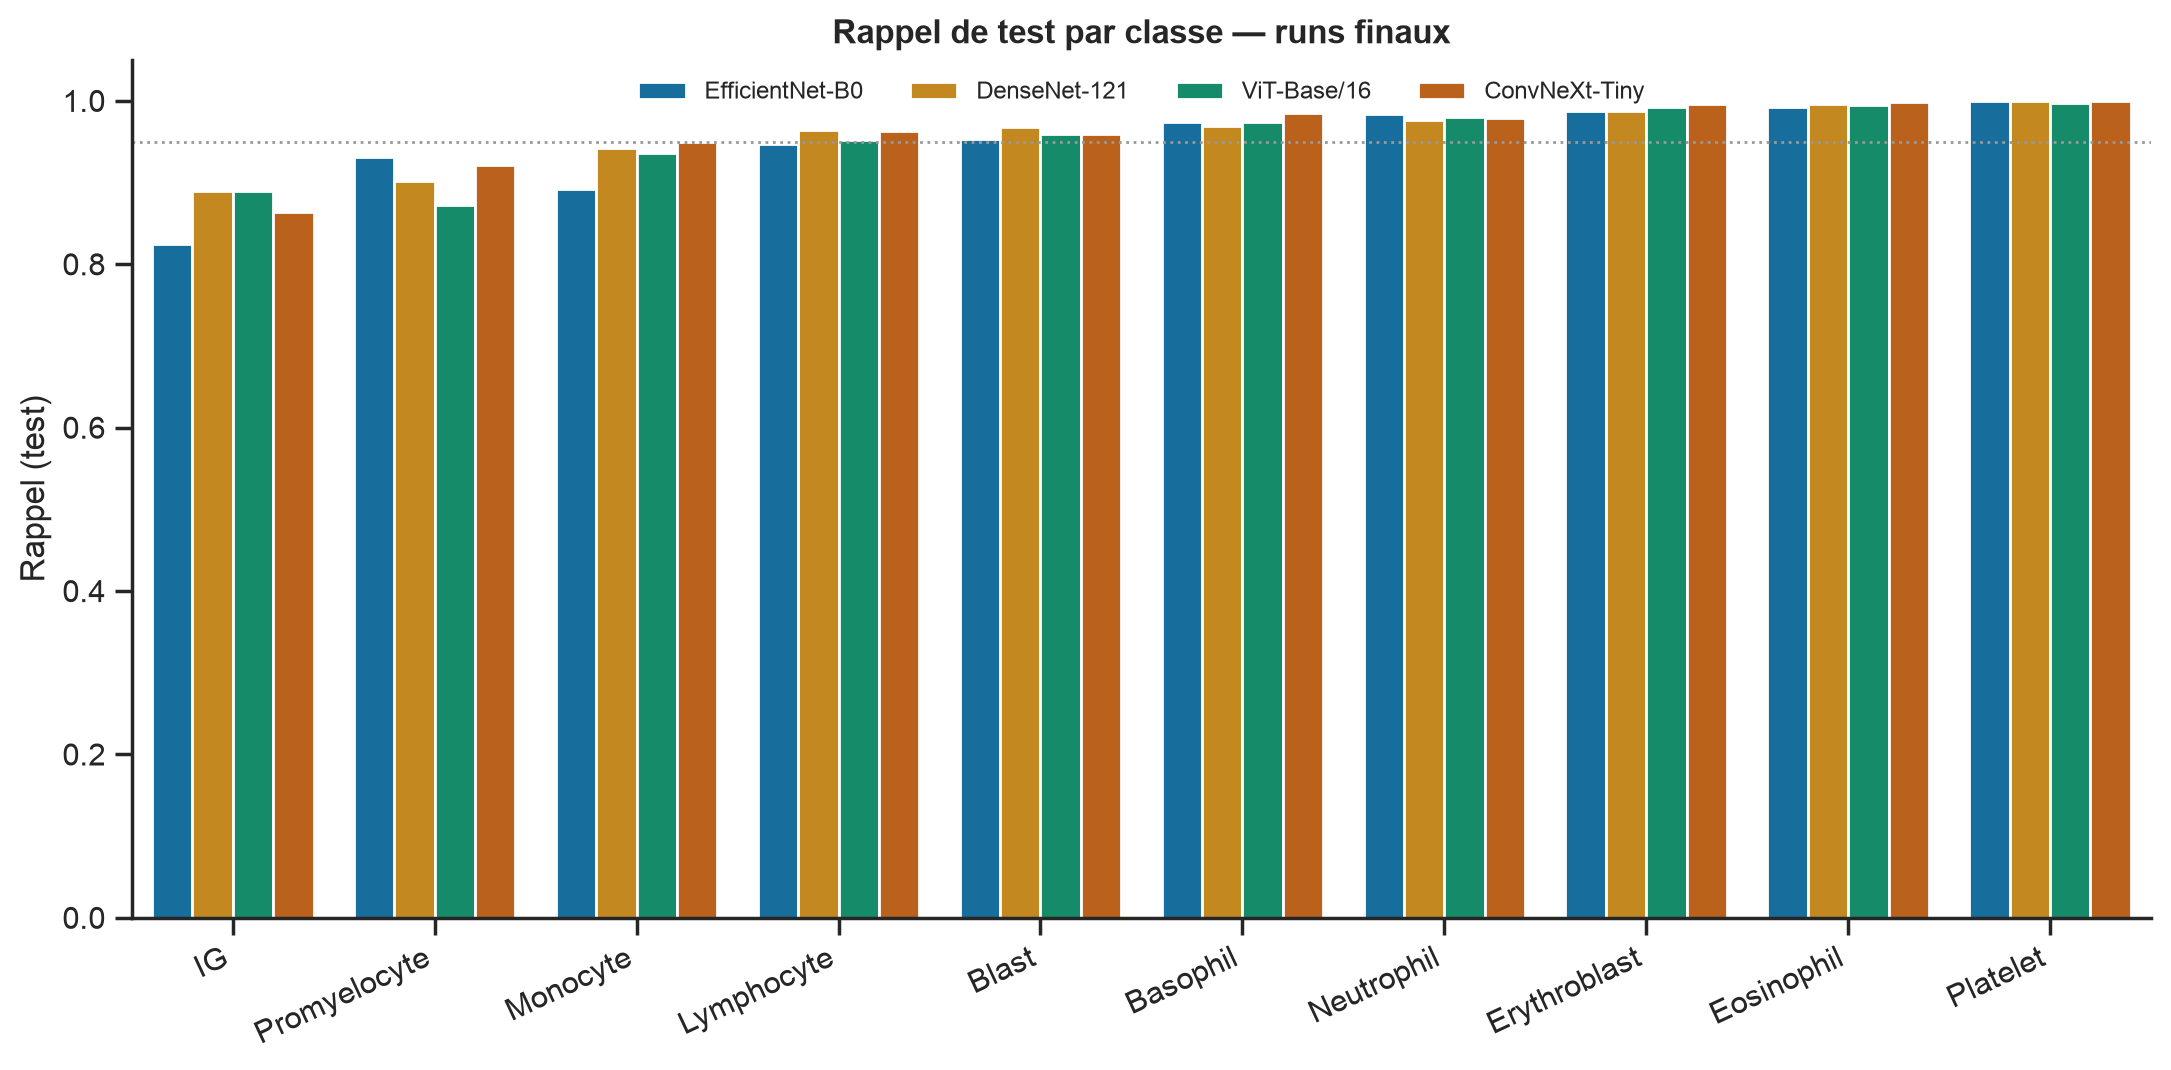
\includegraphics[width=0.85\linewidth]{report/transfer_final_per_class_recall.png}
  \caption{Rappel de test par classe des 4 runs finaux, triées par rappel croissant pour DenseNet-121. Le repère horizontal marque un rappel de 0,95.}
  \label{fig:transfer-final-per-class-recall}
\end{figure}

La figure~\ref{fig:transfer-final-per-class-recall} confirme que les granulocytes immatures (IG) et le promyélocyte restent, pour les 4 modèles, les deux classes les plus difficiles, cohérent avec les confusions déjà observées sur la \emph{baseline} (\S~\ref{sec:baseline}) entre promyélocyte, blaste et IG.
Sur toutes les autres classes, les 4 modèles dépassent 0,89 de rappel, et la majorité franchit 0,95.

\begin{figure}[H]
  \centering
  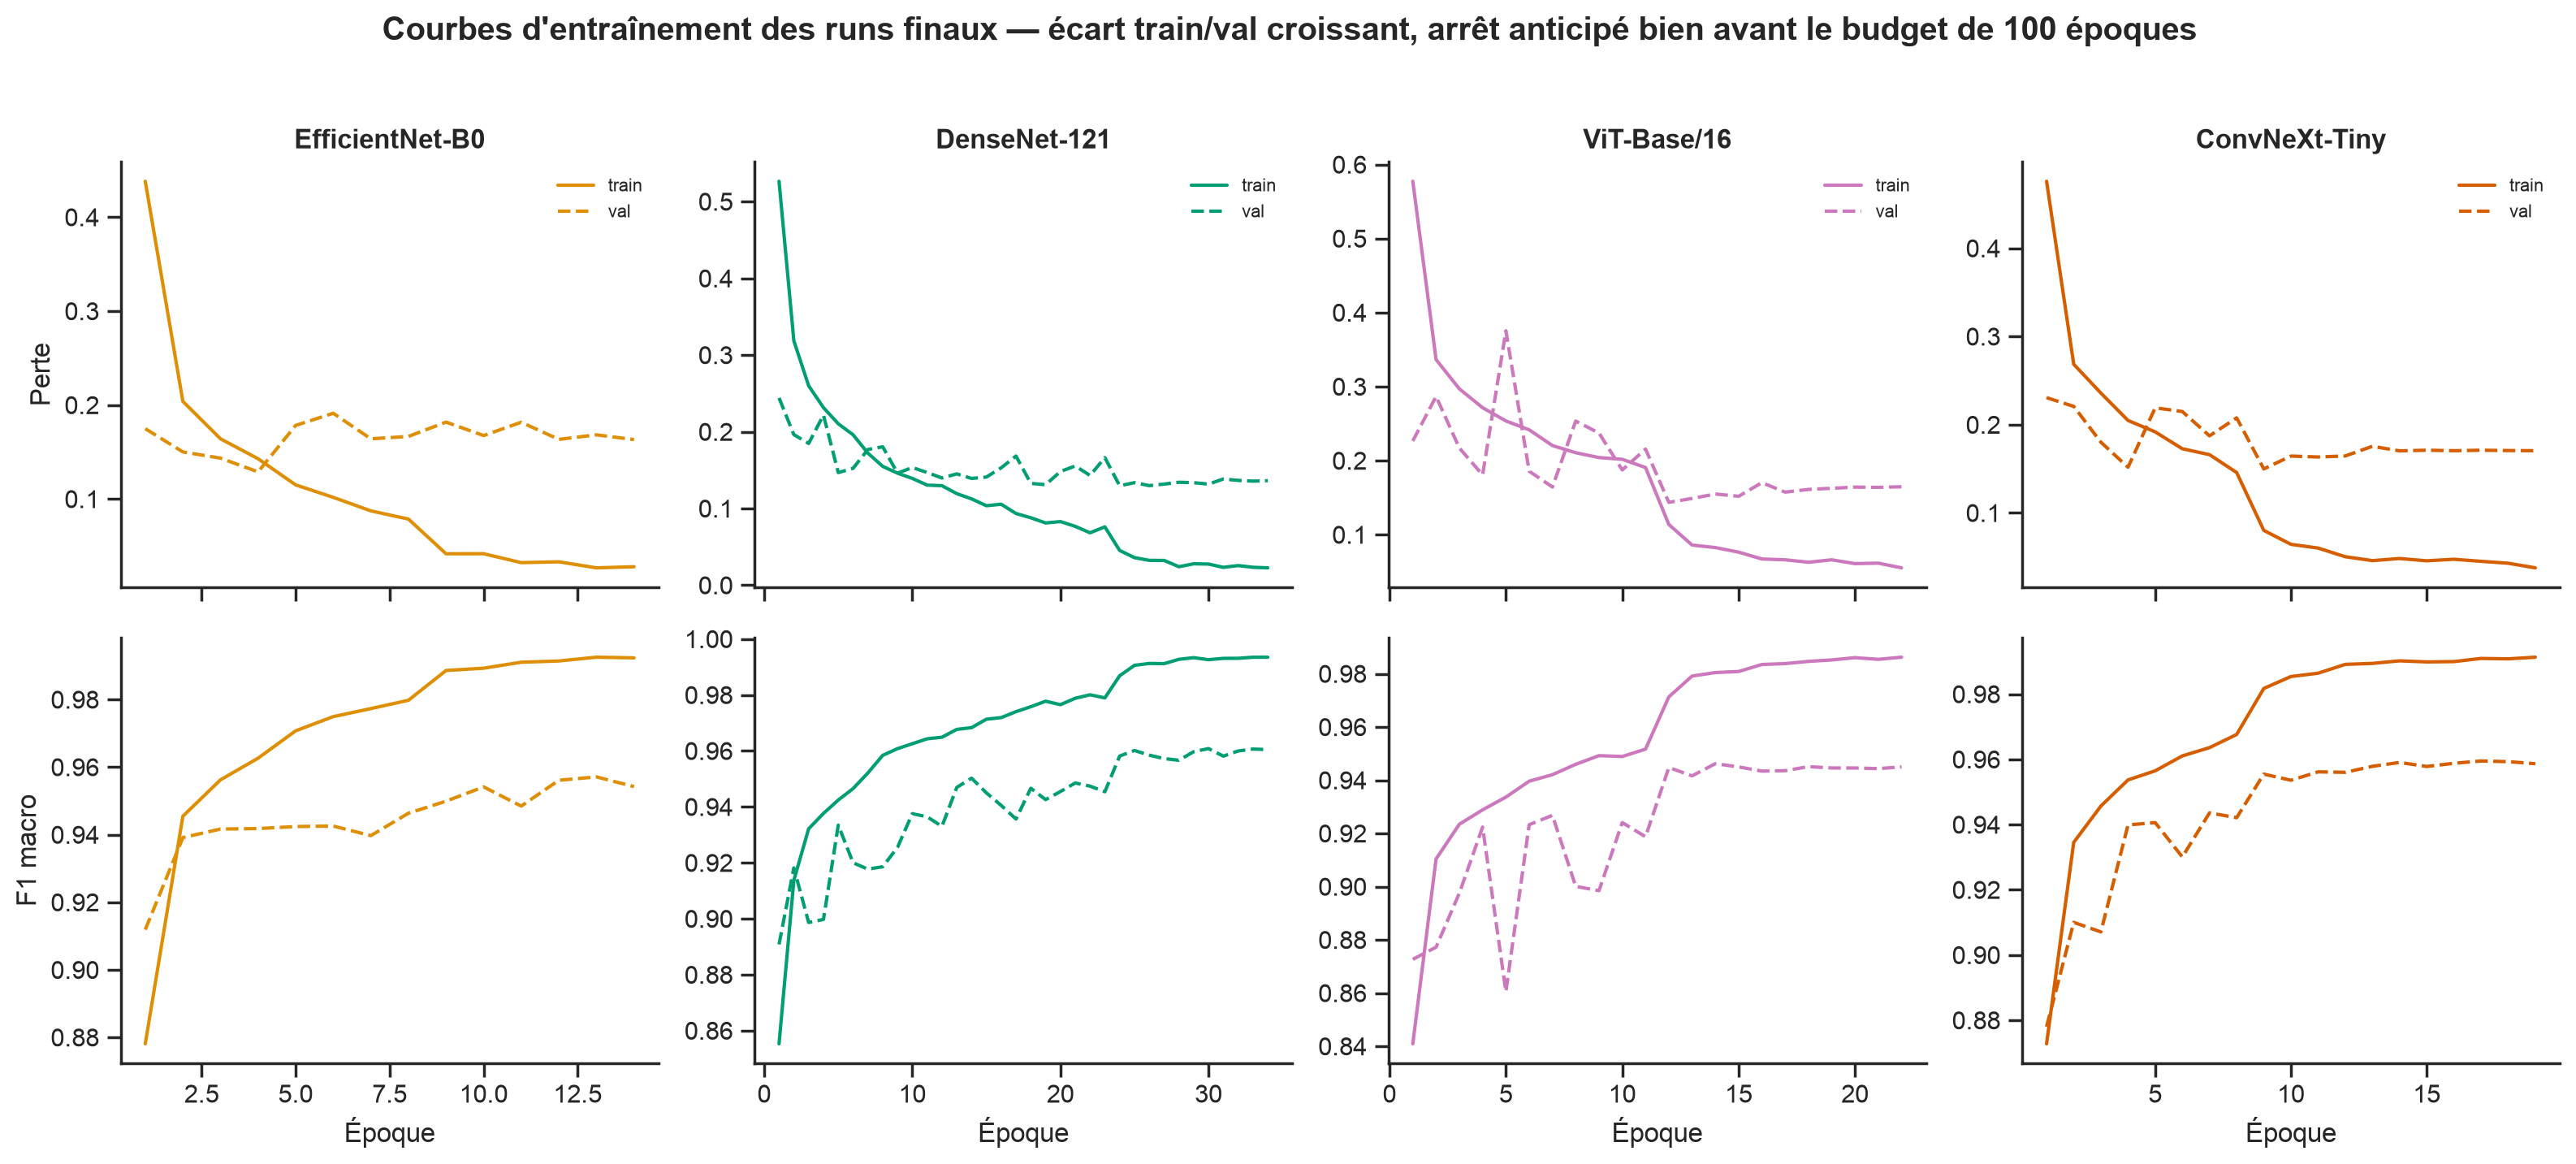
\includegraphics[width=\linewidth]{report/transfer_final_training_curves.png}
  \caption{Courbes d'entraînement (perte et F1 macro, train / validation) des 4 runs finaux.}
  \label{fig:transfer-final-training-curves}
\end{figure}

La figure~\ref{fig:transfer-final-training-curves} explique l'arrêt anticipé bien avant le budget de 100 époques (14, 34, 22 et 19 époques respectivement) : dès les premières époques, la perte d'entraînement continue de baisser régulièrement (jusqu'à $\approx$0,02--0,06) tandis que la perte de validation stagne, voire ré-augmente ponctuellement (ViT-Base/16, plus instable), autour de 0,13--0,18.
Le F1 macro suit le même schéma : le score d'entraînement dépasse 0,98--0,99 alors que la validation plafonne entre 0,94 et 0,96, un écart train/validation qui se creuse continûment : la signature classique d'un \textbf{surapprentissage}.
Contrairement au fine-tuning à backbone gelé, dégeler entièrement un extracteur pré-entraîné de plusieurs millions de paramètres sur un jeu de 35\,457 images (dont $\approx$70\,\% utilisées pour l'entraînement) laisse au modèle largement de quoi mémoriser les exemples d'entraînement avant que la représentation apprise ne généralise davantage ; le \emph{scheduler} \texttt{plateau} réduit alors le taux d'apprentissage sur la perte de validation stagnante, ce qui accélère encore la baisse de la perte d'entraînement sans bénéfice supplémentaire côté validation, jusqu'à l'arrêt anticipé (patience de 10 époques sans amélioration).
Ce comportement n'est pas propre à un backbone : il apparaît aux quatre modèles, avec une intensité variable (DenseNet-121, le plus grand nombre d'époques, montre l'écart train/validation le plus progressif ; ViT-Base/16, le plus instable en tout début d'entraînement ; ConvNeXt-Tiny suit un schéma proche de celui de DenseNet-121, avec un écart qui se creuse plus progressivement).

En résumé, le transfert d'apprentissage, en particulier avec un fine-tuning complet du backbone, améliore nettement les performances par rapport à la \emph{baseline} et à l'exploration architecturale \emph{from scratch}, au prix d'un entraînement plus court que prévu (arrêt bien avant le budget de 100 époques) et d'une vigilance accrue sur le surapprentissage une fois le backbone entièrement dégelé.

\subsubsection{Modèle hiérarchique}
\label{sec:modele-hierarchique}

La modélisation binaire par cellule (\S~\ref{sec:modele-binaire}) a mis en évidence une hétérogénéité forte de séparabilité selon les classes : certaines populations (plaquette, éosinophile) se distinguent presque parfaitement du reste, d'autres (promyélocyte, myélocyte, métamyélocyte) restent ambiguës y compris à l'\oe{}il, en raison de leur proximité morphologique sur un même axe de maturation.
Un classifieur \emph{plat} à 10 classes (\S~\ref{sec:baseline}--\S~\ref{sec:transfer-learning}) traite ces deux régimes de difficulté avec la même capacité et le même seuil de décision.
Le modèle hiérarchique explore l'hypothèse inverse : \textbf{router} successivement chaque image à travers une cascade de classifieurs de plus en plus spécialisés, en isolant tôt les classes bien séparées, pour lesquelles une décision \emph{argmax} directe suffit, et en ne réservant les niveaux profonds, coûteux à calibrer, qu'aux classes réellement ambiguës.

\paragraph{Taxonomie fine et rattachement à la nomenclature commune}

Le modèle hiérarchique est entraîné sur une taxonomie plus fine que les \textbf{10 classes} communes au projet (tableau~\ref{tab:fusion-taxonomie}) : \textbf{14 classes}, qui rouvrent la classe \emph{Blaste} en myéloblaste et monoblaste, et la classe \emph{Granulocytes immatures} en myélocyte, métamyélocyte et \emph{IG} (l'étiquette générique, non sous-typée, de PBC).
Ce choix est directement motivé par la cascade elle-même : regrouper myéloblaste et monoblaste \emph{avant} le routage empêcherait d'isoler le premier (bien séparé) du second (21 images seulement, cliniquement critique mais numériquement trop rare pour peser sur un seuil commun).
Le tableau~\ref{tab:hierarchique-taxonomie} détaille le rattachement inverse, utilisé pour toute comparaison avec les autres approches du projet (\S~\ref{sec:resultats-hierarchique}).

\begin{table}[H]
  \centering
  \small
  \renewcommand{\arraystretch}{1.15}
  \begin{tabular}{@{}ll@{}}
    \toprule
    \textbf{Classe commune (10)} & \textbf{Classes fines du modèle hiérarchique (14)} \\
    \midrule
    Blaste                  & Myéloblaste, Monoblaste \\
    Granulocytes immatures  & Myélocyte, Métamyélocyte, IG (PBC, non sous-typé) \\
    Neutrophile              & Neutrophile band, Neutrophile segmenté \\
    Promyélocyte, Éosinophile, Érythroblaste, & \multirow{2}{*}{identiques (correspondance 1:1)} \\
    Lymphocyte, Monocyte, Plaquette, Basophile & \\
    \bottomrule
  \end{tabular}
  \caption{Rattachement des 14 classes fines du modèle hiérarchique aux 10 classes communes du projet (tableau~\ref{tab:fusion-taxonomie}).}
  \label{tab:hierarchique-taxonomie}
\end{table}

\paragraph{Architecture en cascade}

La cascade compte \textbf{5 niveaux} (figure~\ref{fig:hierarchique-cascade}), chacun un \texttt{EfficientNet-B0} pré-entraîné ImageNet distinct, fine-tuné en 2 phases (tête seule à backbone gelé, puis dégel des dernières couches à faible taux d'apprentissage), selon la même logique de transfert que \S~\ref{sec:transfer-learning}, appliquée cette fois à 5 petits classifieurs spécialisés plutôt qu'à un seul classifieur à 10 sorties.

\begin{figure}[H]
  \centering
  \begin{tikzpicture}[
    font=\sffamily\small,
    node distance=6mm and 10mm,
    routeur/.style={draw=lioraink, fill=lioraink!6, rounded corners=2pt, align=center, text width=3.6cm, minimum height=1.05cm, inner sep=4pt},
    terminal/.style={draw=liorared!70, fill=liorared!5, rounded corners=2pt, align=center, text width=4.9cm, minimum height=1.05cm, inner sep=4pt},
    arr/.style={-{Stealth[length=2mm]}, lioragrey, thick}
  ]
  \node[routeur] (n1) {\textbf{Niveau 1}\\6 sorties};
  \node[terminal, right=of n1] (t1) {Plaquette, Érythroblaste, Lymphocyte, Basophile, Monocyte\\\footnotesize(décision directe, pas de rejet)};
  \node[routeur, below=of n1] (n2) {\textbf{Niveau 2}\\Éosinophile vs reste};
  \node[terminal, right=of n2] (t2) {Éosinophile\\\footnotesize(décision directe, pas de rejet)};
  \node[routeur, below=of n2] (n3) {\textbf{Niveau 3}\\3 sorties};
  \node[terminal, right=of n3] (t3) {Neutrophile band / segmenté\\\footnotesize(décision directe, pas de rejet)};
  \node[routeur, below=of n3] (n4) {\textbf{Niveau 4}\\6 sorties, rejet calibré};
  \node[terminal, right=of n4] (t4) {Myéloblaste, Promyélocyte, Myélocyte, Métamyélocyte, Monoblaste, IG};
  \node[routeur, below=of n4] (n5) {\textbf{Niveau 5}\\second avis IG, rejet calibré};
  \node[terminal, right=of n5] (t5) {IG confirmé\\\footnotesize(ou rejeté)};
  \draw[arr] (n1) -- (t1); \draw[arr] (n1) -- (n2);
  \draw[arr] (n2) -- (t2); \draw[arr] (n2) -- (n3);
  \draw[arr] (n3) -- (t3); \draw[arr] (n3) -- (n4);
  \draw[arr] (n4) -- (t4); \draw[arr] (n4) -- (n5);
  \draw[arr] (n5) -- (t5);
  \end{tikzpicture}
  \caption{Architecture de la cascade à 5 niveaux. Chaque flèche descendante correspond au sous-groupe encore ambigu après le niveau courant ; chaque flèche vers la droite à une décision terminale.}
  \label{fig:hierarchique-cascade}
\end{figure}

Le routage suit l'ordre de difficulté croissante observé en \S~\ref{sec:modele-binaire} : le Niveau~1 isole d'abord les 5 classes les mieux séparées du reste (le groupe granulocytaire, 9 classes) ; le Niveau~2 en extrait l'éosinophile (granulations très caractéristiques) ; le Niveau~3 sépare les deux formes de neutrophile matures des formes immatures ; le Niveau~4, le \emph{n\oe{}ud dur} de la cascade, tranche entre les 6 classes restantes : exactement celles pour lesquelles la modélisation binaire par cellule avait signalé le plus de confusion.
Le Niveau~5 n'est pas un routeur supplémentaire mais une \textbf{vérification a posteriori}, appliquée uniquement aux cas que le Niveau~4 vient de classer \emph{IG} : un second modèle dédié, entraîné à distinguer \emph{IG} du reste, doit confirmer la décision avant qu'elle ne soit acceptée.

\paragraph{Classification sélective et seuils de rejet calibrés}

Plutôt qu'un seuillage post-hoc sur une sortie \emph{softmax} unique (l'approche retenue \S~\ref{sec:limites-loss} et figure~\ref{fig:baseline-critical-screening} pour la \emph{baseline}), la cascade intègre un mécanisme de rejet \textbf{à deux de ses niveaux} (4 et 5, ceux qui portent le plus d'ambiguïté résiduelle) : une image n'est acceptée que si la confiance du modèle dépasse un seuil $T$, calibré séparément par niveau pour garantir une précision cible sur les cas acceptés (\texttt{TARGET\_PRECISION}, 0,95 au Niveau~4 et 0,97 au Niveau~5) ; en deçà, elle est étiquetée \og à confirmer manuellement \fg{} plutôt que forcée vers une classe.
Les Niveaux~1 à~3 ne portent volontairement aucun rejet : appliqué à des classes déjà bien séparées, un seuil calibré sur l'ensemble du groupe s'est révélé contre-productif en pratique : il pénalise des classes faciles pour compenser des classes difficiles avec lesquelles elles n'ont rien en commun.
Ce compromis couverture/fiabilité, ajustable via la précision cible, joue pour la cascade le même rôle que le réglage de seuil de la figure~\ref{fig:baseline-critical-screening} pour la \emph{baseline}, mais \emph{intégré} à l'architecture plutôt qu'appliqué après coup sur une seule sortie.

\paragraph{Résultats}
\label{sec:resultats-hierarchique}

Le tableau~\ref{tab:hierarchique-niveaux} détaille la performance de validation de chaque niveau et le seuil de rejet retenu là où il s'applique.

\begin{table}[H]
  \centering
  \small
  \renewcommand{\arraystretch}{1.15}
  \begin{tabular}{@{}lrrl@{}}
    \toprule
    Niveau & Accuracy val.\ (Phase 2) & Seuil de rejet $T$ & Précision cible \\
    \midrule
    1 : routeur grossier         & 0,977 & n. a. & n. a. \\
    2 : Éosinophile vs reste     & 0,997 & n. a. & n. a. \\
    3 : band / segmenté / reste  & 0,948 & n. a. & n. a. \\
    4 : n\oe{}ud dur (6 classes) & 0,852 & 0,809 & 0,95 \\
    5 : second avis IG           & 1,000 & 0,651 & 0,97 \\
    \bottomrule
  \end{tabular}
  \caption{Performance de validation par niveau et seuils de rejet calibrés retenus.}
  \label{tab:hierarchique-niveaux}
\end{table}

Sur le jeu de test complet (14 classes), la cascade rend une décision ferme pour \textbf{93,6\,\%} des images, avec une accuracy de \textbf{94,2\,\%} sur ces décisions ; en comptant les rejets comme des erreurs, l'accuracy globale est de \textbf{88,2\,\%}.
La figure~\ref{fig:hierarchique-confusion-14} détaille la matrice de confusion complète.

\begin{figure}[H]
  \centering
  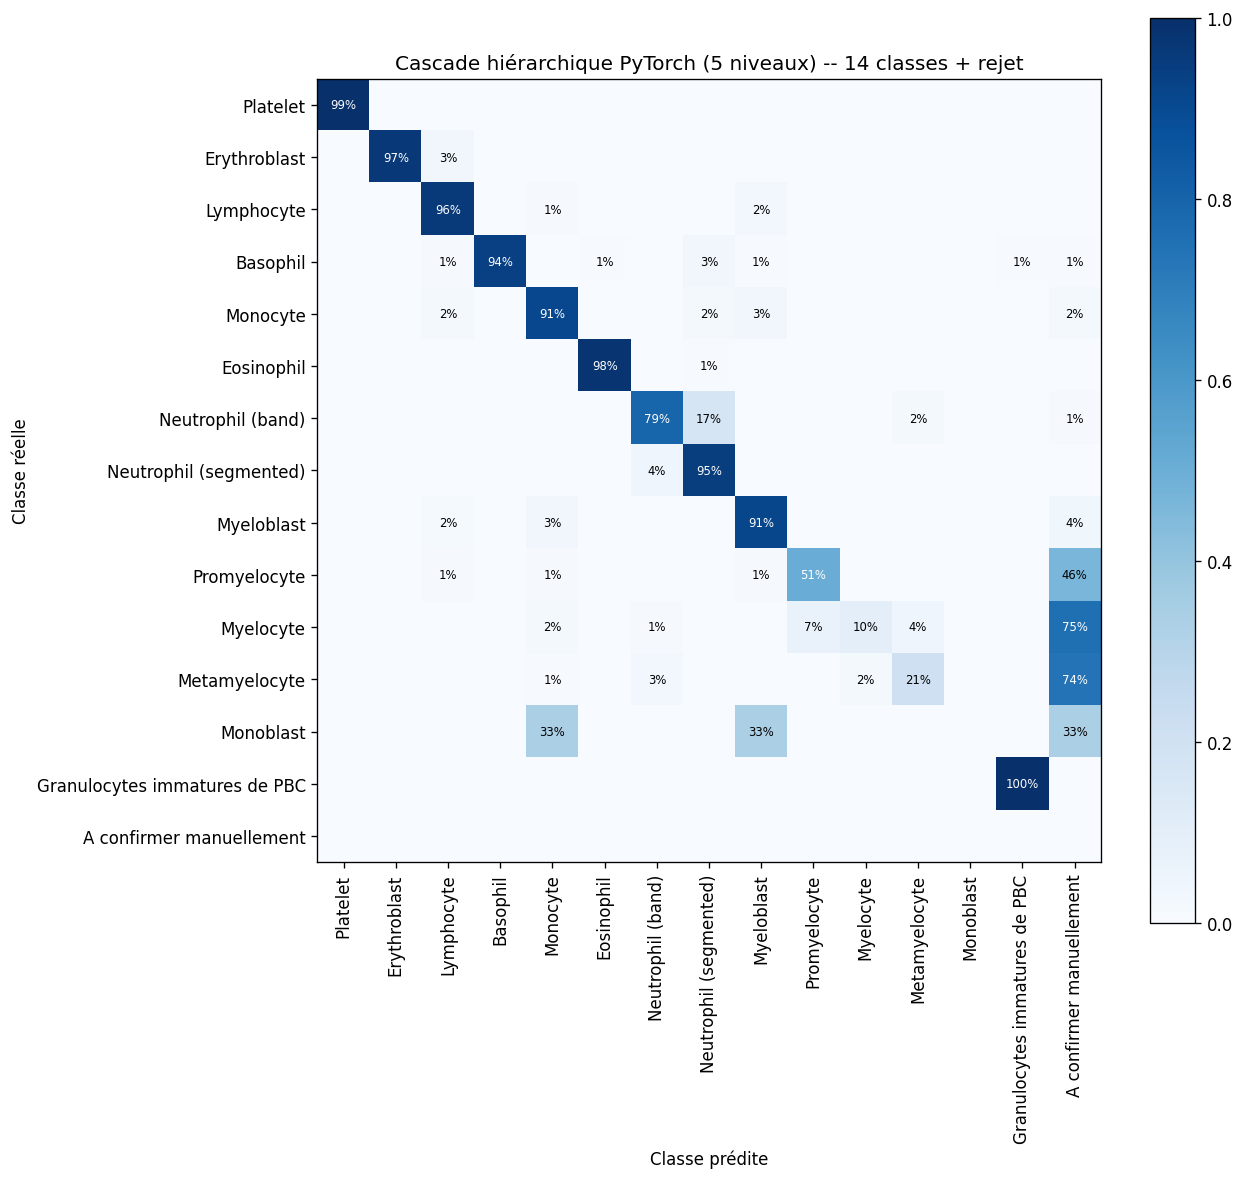
\includegraphics[width=\linewidth]{report/hierarchique_confusion_14classes.png}
  \caption{Matrice de confusion de test, taxonomie fine à 14 classes (normalisée par ligne).}
  \label{fig:hierarchique-confusion-14}
\end{figure}

Le clivage annoncé au paragraphe précédent se confirme intégralement : les classes sans rejet (Niveaux 1--3) atteignent 91 à 99\,\% de rappel direct, tandis que le n\oe{}ud dur (Niveau~4) reste le point faible de la cascade : myélocyte et métamyélocyte, en particulier, sont rejetées dans 3 cas sur 4 plutôt que mal classées, cohérent avec l'objectif du seuil calibré (préférer un rejet à une erreur silencieuse) mais révélateur d'une difficulté que l'architecture atténue sans la résoudre.
Le monoblaste (0\,\% de rappel, 21 images de test réparties à parts égales entre monocyte, myéloblaste et rejet) reste, comme en \S~\ref{sec:baseline}, hors d'atteinte d'un simple réglage de seuil : sa rareté numérique, déjà signalée lors de la fusion des taxonomies (\S~\ref{sec:pre-processing-feature-engineering}), est le facteur limitant, pas l'architecture.
Le second avis du Niveau~5, en revanche, confirme \emph{IG} avec 100\,\% de rappel sur ce jeu de test : un résultat interrogé plus loin (\S~\ref{sec:resultats-gradcam}).

\paragraph{Configuration retenue et pistes explorées}

L'architecture à 5 niveaux ci-dessus est la \textbf{configuration retenue} pour les résultats et comparaisons de ce rapport (\S~\ref{sec:resultats-hierarchique}, \S~\ref{sec:resultats-gradcam}) : c'est celle disposant d'une évaluation complète (métriques de test, remappage vers la nomenclature commune et diagnostic Grad-CAM) et donc la seule comparable aux autres approches du projet.
Plusieurs raffinements ont par ailleurs été explorés en cours de projet sans être intégrés à cette configuration de référence, chacun avec un statut différent à date~:
\begin{itemize}
  \item un \textbf{niveau supplémentaire} isolant le myéloblaste du n\oe{}ud dur (Niveau 4) dans un gate binaire dédié, pour lui donner un seuil de rejet propre plutôt que partagé avec des classes bien plus difficiles~: gain net sur le myéloblaste (jusqu'à 94\,\% de rappel) mais sans confirmation, à ce stade, que l'architecture à 6 niveaux dépasse la version à 5 niveaux \emph{une fois toutes les autres pistes contrôlées} ;
  \item une \textbf{normalisation de coloration inter-sites} (transfert de statistiques dans l'espace LAB), motivée par le risque de raccourci de site déjà signalé (\S~\ref{sec:pre-processing-feature-engineering}) et par le diagnostic Grad-CAM du \S~\ref{sec:resultats-gradcam}~: sans régression mesurée sur les niveaux testés, mais sans preuve, non plus, qu'elle corrige le raccourci identifié sur \emph{IG} : cohérent avec l'hypothèse que ce raccourci tient autant à des artefacts de compression qu'à la seule coloration ;
  \item une \textbf{augmentation de données ciblée} (retournements et zooms, proportionnelle à la rareté de chaque classe) sur les classes du n\oe{}ud dur~: a mesurablement amélioré l'accuracy de validation du Niveau~4, sans encore avoir été combinée aux deux pistes précédentes dans une seule configuration finale.
\end{itemize}  
Ces trois pistes sont \textbf{indépendantes et cumulables} : chacune a été validée isolément, mais leur combinaison, et sa comparaison rigoureuse à la configuration retenue ici, reste à mener pour la suite du projet, en particulier avant tout déploiement s'appuyant sur la classe \emph{IG}.

\subsection{Résultats}
\label{sec:resultats}

\subsubsection{Interprétabilité par Grad-CAM}
\label{sec:resultats-gradcam}

Pour vérifier que chaque niveau de la cascade fonde sa décision sur la morphologie cellulaire plutôt que sur un artefact de source (risque déjà identifié \S~\ref{sec:pre-processing-feature-engineering} et \S~\ref{sec:modele-binaire}), une carte de saillance \textbf{Grad-CAM} \parencite{selvaraju2017gradcam} est calculée pour une image de test de chacune des 14 classes fines, sur la dernière couche de convolution du niveau responsable de sa décision (figure~\ref{fig:hierarchique-cascade}).

\begin{figure}[H]
  \centering
  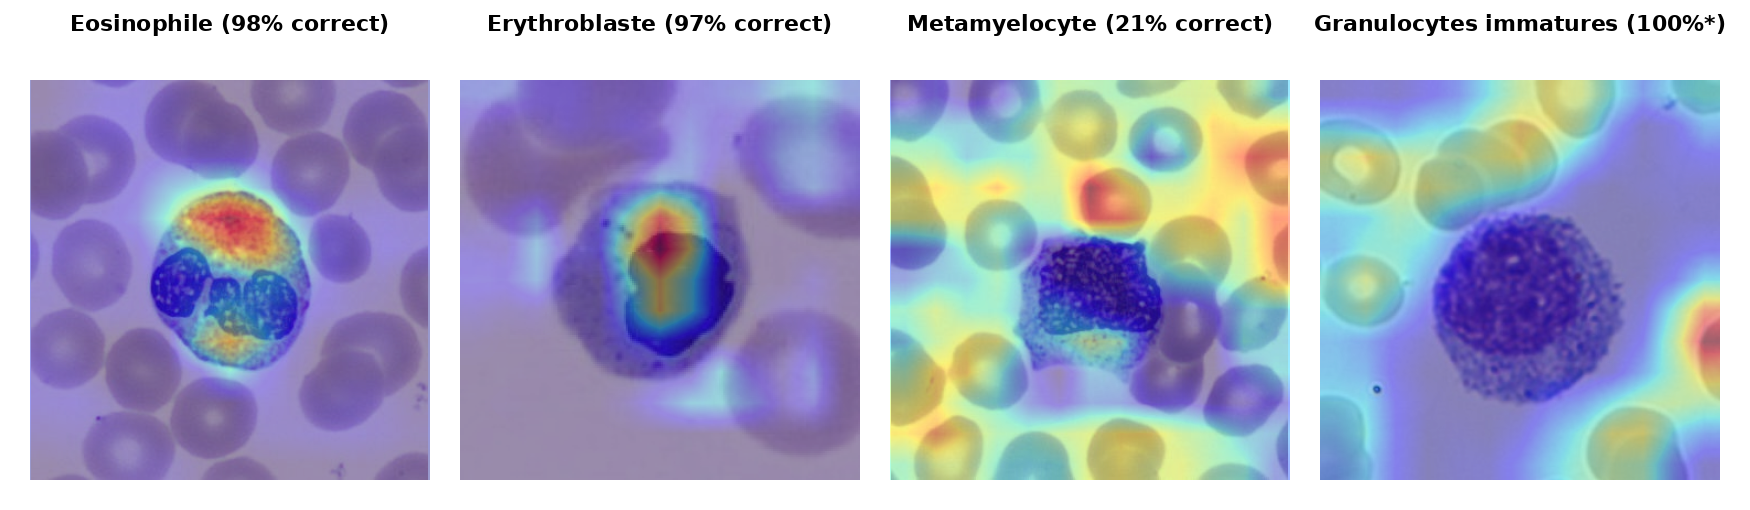
\includegraphics[width=\linewidth]{report/hierarchique_gradcam_comparaison.png}
  \caption{Superposition Grad-CAM (rouge = activation forte, bleu = activation faible) pour quatre classes représentatives. De gauche à droite : deux classes bien classées (Niveaux 1--2, localisation propre sur la cellule), une classe du n\oe{}ud dur en difficulté (Niveau 4) et \emph{IG} (Niveau 4, second avis Niveau 5).}
  \label{fig:hierarchique-gradcam}
\end{figure}

Le résultat est net et corrèle directement avec la performance par classe.
Pour les classes bien séparées (éosinophile, érythroblaste, et plus généralement les Niveaux 1 à 3), le foyer d'activation se superpose fidèlement à la cellule annotée (sur ses granulations pour l'éosinophile, sur la frontière du noyau dense pour l'érythroblaste) : le modèle fonde bien sa décision sur une caractéristique morphologique interprétable.
Pour plusieurs classes du n\oe{}ud dur en difficulté (myélocyte, métamyélocyte), l'activation se déplace au contraire vers des hématies du fond, sans rapport avec la cellule cible : un signe que le modèle peine à identifier un repère visuel fiable, cohérent avec leur taux de rejet élevé (figure~\ref{fig:hierarchique-confusion-14}) plutôt qu'une simple insuffisance de données.

\textbf{Le cas le plus significatif concerne \emph{IG}.}
Alors que le Niveau~5 confirme cette classe avec 100\,\% de rappel (\S~\ref{sec:resultats-hierarchique}), un score qui, isolément, semblerait excellent, la carte Grad-CAM correspondante (figure~\ref{fig:hierarchique-gradcam}, à droite) montre que la cellule elle-même se situe dans la zone la \emph{moins} activée de l'image : le modèle fonde sa décision presque exclusivement sur des hématies environnantes.
Ce résultat corrobore directement, par une méthode indépendante, l'hypothèse déjà formulée à la fusion des taxonomies (\S~\ref{sec:pre-processing-feature-engineering}, cf.\ \hyperref[par:jpeg-artefacts]{artefacts de compression JPEG}) : les artefacts de compression JPEG propres à PBC constituent un indicateur de site quasi parfait, que le modèle peut apprendre à la place de la morphologie cellulaire.
La classe \emph{IG} en est un candidat particulièrement exposé : son équivalent fin (myélocyte/métamyélocyte) est très majoritairement issu de LMU (tableau~\ref{tab:fusion-taxonomie}), et son score de 100\,\% de rappel doit donc être lu comme un \textbf{signal d'alerte plutôt qu'une performance à retenir}, tant que le test de contrôle \og PBC contre LMU \fg{} déjà anticipé (\S~\ref{sec:pre-processing-feature-engineering}) n'a pas isolé la part de ce score imputable au site d'acquisition.

En résumé, Grad-CAM apporte ici un diagnostic que les métriques ne révèlent pas seules : une bonne performance ponctuelle peut coexister avec un fondement morphologique absent, tandis qu'une performance médiocre (myélocyte, métamyélocyte) s'accompagne ici d'un signe cohérent : une localisation déjà dégradée.
Cette lecture renforce la recommandation du \S~\ref{sec:pre-processing-feature-engineering} : avant tout déploiement, un test de contrôle par source doit être mené sur les classes les plus exposées au biais de site, \emph{IG} en tête.

\subsubsection{Comparaison des approches}

Les trois approches ayant abouti à un run final, \emph{baseline} (\S~\ref{sec:baseline}), transfert d'apprentissage (\S~\ref{sec:transfer-learning}) et modèle hiérarchique (\S~\ref{sec:modele-hierarchique}), ne sont pas entraînées sur une architecture ni, pour la cascade, une taxonomie strictement identique ; leur comparaison directe demande donc de ramener le modèle hiérarchique, entraîné sur 14 classes, à la nomenclature commune à 10 classes (tableau~\ref{tab:hierarchique-taxonomie}), par remontée des probabilités le long de la cascade\footnote{Chaque n\oe{}ud de la cascade produit une probabilité conditionnelle sachant que l'image l'a atteint ; leur produit le long de chaque chemin racine\,$\to$\,feuille donne, pour chaque image, une probabilité marginale sur les 14 classes fines, sommées ensuite par classe commune. Cette reconstruction ne s'applique qu'au calcul des métriques de comparaison : la décision opérationnelle de la cascade (tableau~\ref{tab:hierarchique-niveaux}) reste celle, avec rejet, du \S~\ref{sec:resultats-hierarchique}.}.
Le tableau~\ref{tab:comparaison-approches} rassemble les métriques ainsi rendues comparables.

\begin{table}[H]
  \centering
  \small
  \renewcommand{\arraystretch}{1.2}
  \begin{tabularx}{\textwidth}{@{}>{\raggedright\arraybackslash}Xrrrr@{}}
    \toprule
    Approche & F1 macro & MCC & Top-3 acc. & Rappel promyélocyte \\
    \midrule
    Baseline (\S~\ref{sec:baseline})             & 0,916 & 0,932 & 0,995 & 0,843 \\
    Transfer learning, ConvNeXt-Tiny (\S~\ref{sec:transfer-learning}) & 0,949 & 0,961 & 0,998 & 0,922 \\
    Modèle hiérarchique (\S~\ref{sec:modele-hierarchique}, remappé 10 classes) & 0,944 & 0,959 & 0,993 & 0,753 \\
    \bottomrule
  \end{tabularx}
  \caption{Comparaison des trois approches sur la nomenclature commune à 10 classes.
  ConvNeXt-Tiny est retenu comme représentant du transfert d'apprentissage car son run final est, de très peu, le meilleur des quatre (\S~\ref{sec:transfer-learning}) ; DenseNet-121 obtient des résultats quasi identiques (F1 macro 0,949, MCC 0,961) et resterait un choix tout aussi défendable.
  Le rappel promyélocyte du modèle hiérarchique est calculé sur l'ensemble du test (sans restriction aux décisions fermes), pour rester comparable au rappel \emph{par classe} des deux autres approches.}
  \label{tab:comparaison-approches}
\end{table}

Sur les métriques globales, la complexité architecturale ne prédit pas la performance : la \emph{baseline} (petit CNN maison, $\approx$3,0\,M paramètres, sans pré-entraînement) est certes la plus faible partout, mais le modèle hiérarchique, pourtant cinq backbones EfficientNet-B0 distincts chacun ré-affiné séparément, ne fait que se situer entre les deux autres, sans dépasser le transfert d'apprentissage qui n'utilise qu'un unique backbone : la spécialisation par niveau ne compense donc pas ici le surcoût architectural, ni l'avantage d'un classifieur unique disposant de la totalité du signal d'entraînement à chaque décision.

L'écart le plus net porte sur le \textbf{rappel du promyélocyte} : 0,922 pour le transfert d'apprentissage, 0,843 pour la \emph{baseline}, et seulement 0,753 pour le modèle hiérarchique une fois les rejets comptés comme des erreurs.
Ce dernier chiffre doit toutefois être relativisé : au sein du n\oe{}ud dur de la cascade, cette classe rare (647 images d'entraînement, la plus rare du groupe avec le monoblaste) est régulièrement \emph{rejetée} plutôt que mal classée (\S~\ref{sec:resultats-hierarchique}) : un rappel \og sans rejet \fg{} pénalise ce comportement alors qu'en usage réel un rejet déclenche une relecture humaine, pas une erreur silencieuse comme pour les deux autres approches.

Les trois approches diffèrent aussi dans leur manière de gérer l’incertitude : la \emph{baseline} et le transfert d'apprentissage tranchent par \emph{argmax}, avec un ajustement de seuil possible en post-traitement sur un score global (\S~\ref{sub:metriques}, figure~\ref{fig:baseline-critical-screening}) ; le modèle hiérarchique intègre à la place un mécanisme de rejet calibré niveau par niveau (\S~\ref{sec:resultats-hierarchique}) et donne accès à \textbf{quelle sous-décision} de la cascade explique une erreur, plutôt qu'une confusion agrégée entre 10 classes, au prix d'un pipeline d'entraînement et d'évaluation sensiblement plus complexe, pour une performance brute qui ne dépasse pas celle d'un unique backbone transféré.

\subsubsection{Comparaison aux références de la littérature}
\label{sec:comparaison-litterature}

Le \S~\ref{sec:transfer-learning} (« Modèles de référence dans la littérature ») recensait les travaux qui traitent la même tâche que ce projet ; ils fournissent ici trois points de repère chiffrés, à lire avec prudence puisqu'aucun n'évalue exactement la même taxonomie ni la même fusion de sources.
\textbf{Matek et al.} \parencite{matek2019nmi} atteignent $\approx$90\,\% d'accuracy sur la discrimination binaire blaste / non-blaste, directement sur Matek-19 (LMU) : une tâche plus simple (2 classes, une seule source) que notre \texttt{type} à 10 classes fusionné.
\textbf{Acevedo et al.} \parencite{acevedo2019cnn} rapportent $\approx$96\,\% sur PBC avec VGG-16/InceptionV3 ; des travaux plus récents sur PBC seul (8 classes) atteignent 98--98,6\,\% avec des architectures EfficientNet/DenseNet \parencite{asghar2024tenclasses,asghar2023allbloodcell}.

Sur notre tâche \texttt{type} (10 classes, PBC + LMU fusionnés), le meilleur run final (ConvNeXt-Tiny, transfert d'apprentissage, tableau~\ref{tab:transfer-resultats-finaux}) atteint 96,2\,\% d'accuracy et 0,949 de F1 macro, dans la fourchette haute d'Acevedo et al., mais en retrait des 98--98,6\,\% rapportés par la littérature PBC la plus récente.
Cet écart n'est pas nécessairement imputable au choix d'architecture : ces travaux évaluent sur PBC seul, source homogène à 8 classes, tandis que notre protocole fusionne PBC et LMU, deux sites dont le \emph{domain gap} a été caractérisé en détail (\S~\ref{sec:pre-processing-feature-engineering}), sur une taxonomie à 10 classes qui isole notamment le promyélocyte des autres granulocytes immatures.
Sur la question la plus proche de celle de Matek et al., détecter qu'une cellule est critique quel que soit son type exact, notre rappel critique groupé (\texttt{grouped\_critical\_recall}, \S~\ref{sub:metriques}) atteint 0,963 pour ConvNeXt-Tiny (déjà 0,950 pour la \emph{baseline}, tableau~\ref{tab:baseline-resultats-finaux}), au-dessus des $\approx$90\,\% de Matek et al. C'est un résultat encourageant, mais qui reste une comparaison indicative plutôt qu'un remplacement direct : les deux tâches ne partagent ni la même définition de « critique » ni le même jeu de test.

Le transfert d'apprentissage rapproche donc nettement notre pipeline des références publiées par rapport à la \emph{baseline} seule (92,8\,\% d'accuracy, tableau~\ref{tab:baseline-resultats-finaux}), sans les égaler tout à fait sur la tâche la plus proche de la littérature récente (PBC seul, 8 classes).
Un modèle de fondation spécifique à l'hématologie comme \textbf{DinoBloom} \parencite{koch2024dinobloom}, annoncé par ses auteurs comme dépassant les modèles génériques sur ce type de tâche mais non testé faute de budget de calcul (\S~\ref{sec:transfer-learning}), constituerait la prochaine référence naturelle à confronter à ces résultats.
